\documentclass[10pt,twocolumn,letterpaper]{article}

\usepackage{iccv}
\usepackage{times}
\usepackage{epsfig}
\usepackage{graphicx}
\usepackage{amsmath}
\usepackage{amssymb}
\usepackage{algorithm}
\usepackage{algorithmic}
\usepackage{balance}

% Include other packages here, before hyperref.
\usepackage{bm}

% If you comment hyperref and then uncomment it, you should delete
% egpaper.aux before re-running latex.  (Or just hit 'q' on the first latex
% run, let it finish, and you should be clear).
\usepackage[pagebackref=true,breaklinks=true,letterpaper=true,colorlinks,bookmarks=false]{hyperref}

\iccvfinalcopy % *** Uncomment this line for the final submission

\def\iccvPaperID{4386} % *** Enter the ICCV Paper ID here
\def\httilde{\mbox{\tt\raisebox{-.5ex}{\symbol{126}}}}

% Pages are numbered in submission mode, and unnumbered in camera-ready
\ificcvfinal\pagestyle{empty}\fi
\begin{document}

%%%%%%%%% TITLE
\title{Distributed Lossy Image Compression with Recurrent Networks}

\author{Enmao Diao\\
Duke University\\
{\tt\small enmao.diao@duke.edu}
% For a paper whose authors are all at the same institution,
% omit the following lines up until the closing ``}''.
% Additional authors and addresses can be added with ``\and'',
% just like the second author.
% To save space, use either the email address or home page, not both
\and
Jie Ding\\
University of Minnesota\\
{\tt\small dingj@umn.edu}
\and
Vahid Tarokh\\
Duke University\\
{\tt\small vahid.tarokh@duke.edu}
}

\maketitle
%\thispagestyle{empty}


%%%%%%%%% ABSTRACT
\begin{abstract}
We propose a new architecture for distributed image compression from a group of distributed data sources. The proposed architecture, which we refer to as symmetric Encoder-Decoder Convolutional Recurrent Neural Network, is able to significantly outperform the state-of-the-art compression techniques such as JPEG on rate-distortion curves. We also show that by training distributed encoders and joint decoders on correlated data sources, the performance of compression is much better than that by training codecs separately. For $10$ distributed sources, our distributed system remarkably performs within 2 dB peak signal-to-noise ratio (PSNR) of that of a single codec trained with all data sources. We experiment distributed sources with different correlations and show how our methodology well matches the Slepian-Wolf Theorem in Distributed Source Coding (DSC). Our method is also shown to be robust to the lack of presence of encoded data from a number of distributed sources. To the best of our knowledge, this is the first data-driven DSC framework for general distributed code design with Deep Learning.

\end{abstract}

%%%%%%%%% BODY TEXT
\section{Introduction}
It has been shown by a variety of previous works that Deep Neural Networks (DNN) can achieve comparable results as classical image compression techniques \cite{toderici2015variable,balle2016end,gregor2016towards,toderici2017full,theis2017lossy,johnston2017improved,liu2018cnn}. Most of these methods are based on autoencoder networks and quantization of bottleneck representations, e.g. by quantizing the codes into 8 bit integers and minimizing $\mathcal{L}_1$-penalized loss to sparsify the codes. These models usually rely on entropy codec to compress the sparsified codes. Moreover, to achieve different compression rates, it is unavoidable to train multiple models with different regularization parameters separately.

Among the existing literature of image compression, the recurrent neural network (RNN) based architecture \cite{toderici2015variable} is known to be the pioneering architecture that outperforms classical codecs. The model uses a recurrent autoencoder to encodes the residual difference between the original input and the reconstruction output. At each iteration, new binary coded information is extracted from the residual and the context from previous iterations is stored in the hidden state of the recurrent model. The compression rate, in this case, is varying according to the number of iterations of a single recurrent model. An improved architecture was proposed in \cite{johnston2017improved} that can simultaneously archive spatially adaptive bit rates in a single training phase. 

Motivated by various issues such as data privacy, computational cost, robustness against missing data, the following question has recently gained a lot of research interest. 

\textit{Can distributed encoders perform as well as a single encoder trained with all data sources together?} 

A positive answer from theoretical perspective was given in the context of Distributed Source Coding (DSC). 
In information theory, DSC is an important problem regarding the compression of multiple correlated data sources. The Slepian-Wolf Theorem shows that lossless coding of two or more correlated data sources with separate encoders and a joint decoder can compress data as efficiently as the optimal coding using a joint encoder and decoder \cite{slepian1973noiseless,cover1975proof}. The extension to lossy compression with Gaussian data sources was proposed as Wyner-Ziv Theorem \cite{wyner1976rate}. Although these theorems were published in 1970s, it was after about 30 years that practical applications such as Distributed Source Coding Using Syndromes (DISCUS) emerged \cite{pradhan2003distributed}. One of the main advantages of DSC is that the computation complexity of the encoder is shifted to the decoder. Typically, low complexity encoders can be used in multi-view video coding and sensor networks \cite{girod2005distributed,xiong2004distributed}. 
Motivated by the theoretical development of DSC, in this work we propose a DNN architecture that consists of distributed encoders and a joint decoder. We show that distributed encoders can perform as well as a single encoder trained with all data sources together.
Our proposed DSC framework is data-driven by nature, and it can be applied to distributed data even with unknown correlation structure.

\begin{figure}
\begin{center}
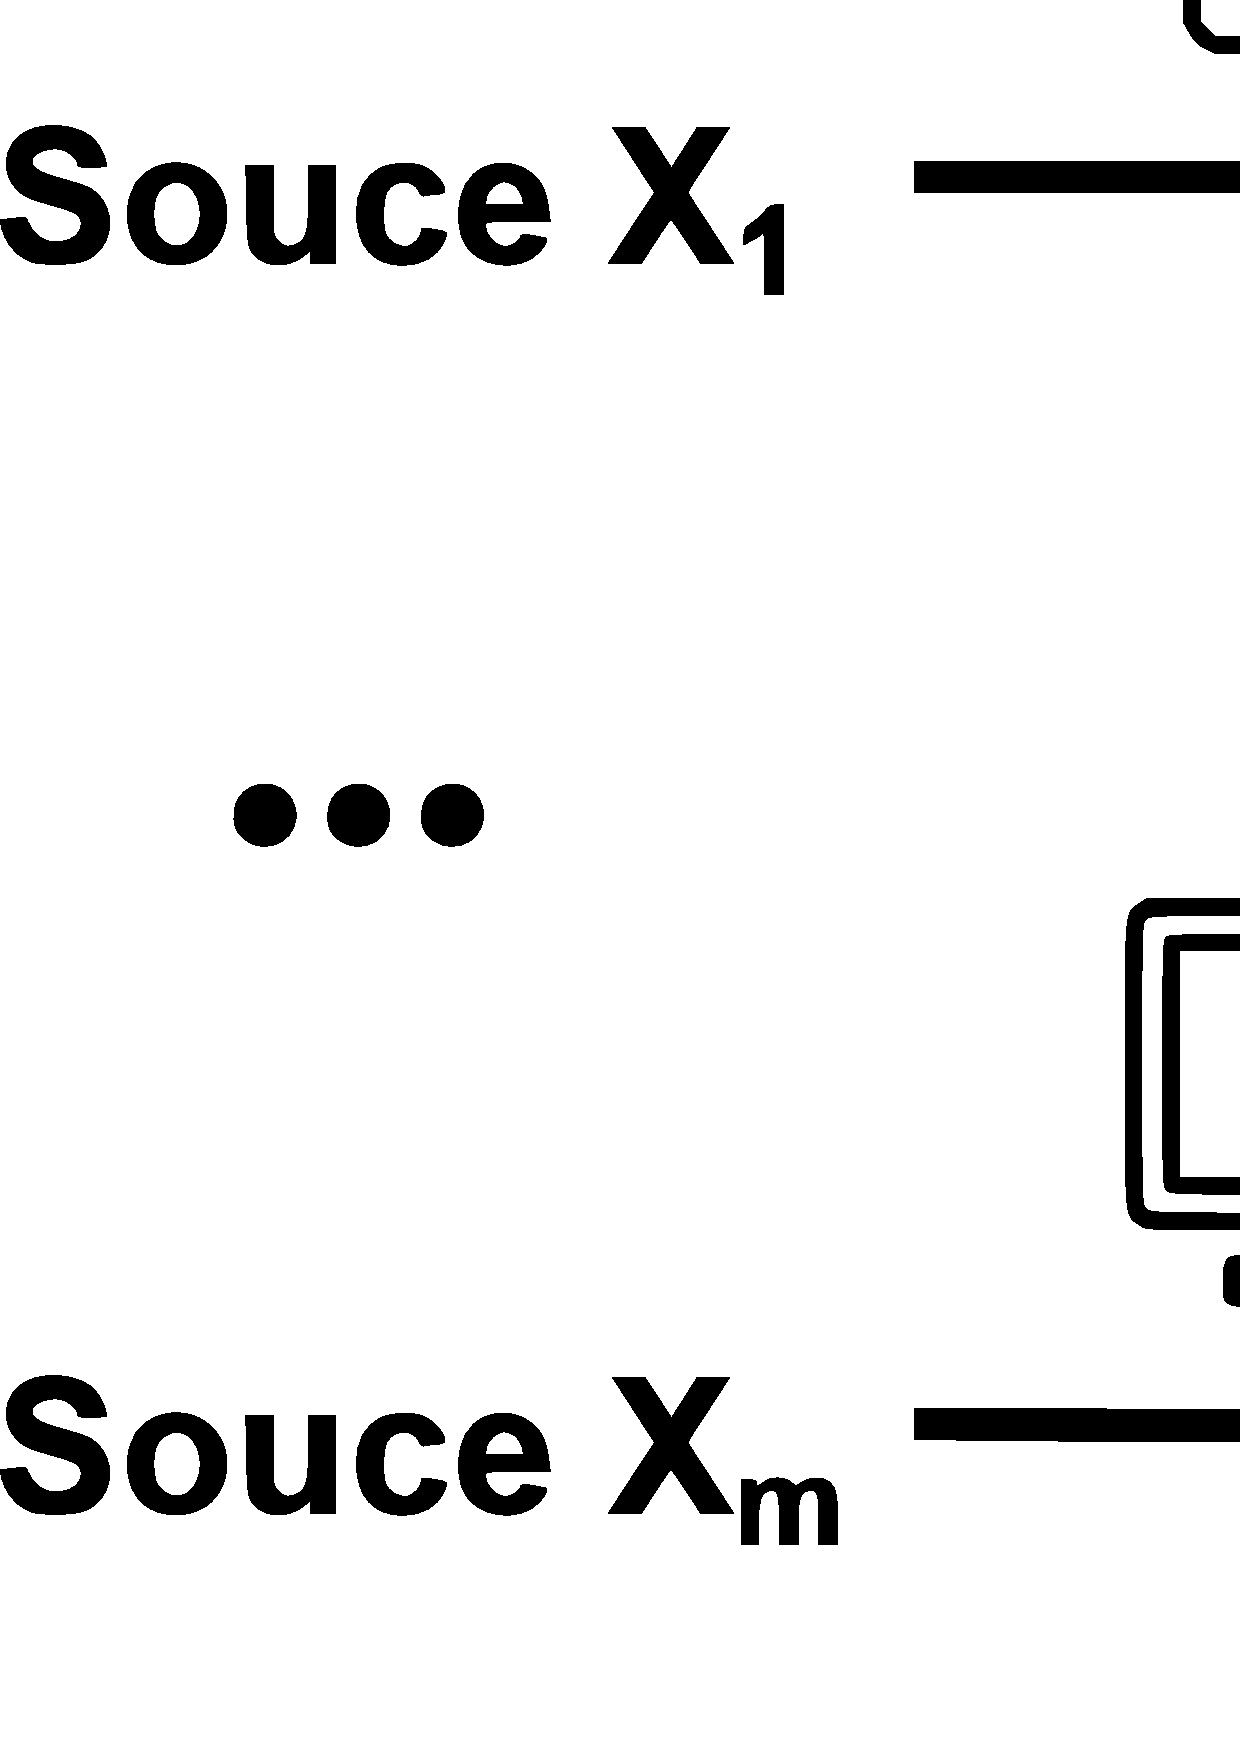
\includegraphics[width=1\linewidth]{DeepDSC.pdf}
\end{center}
   \caption{Illustration of Deep Distributed Source Coding.}
\label{fig_0}
\end{figure}

\begin{figure*}
\begin{center}
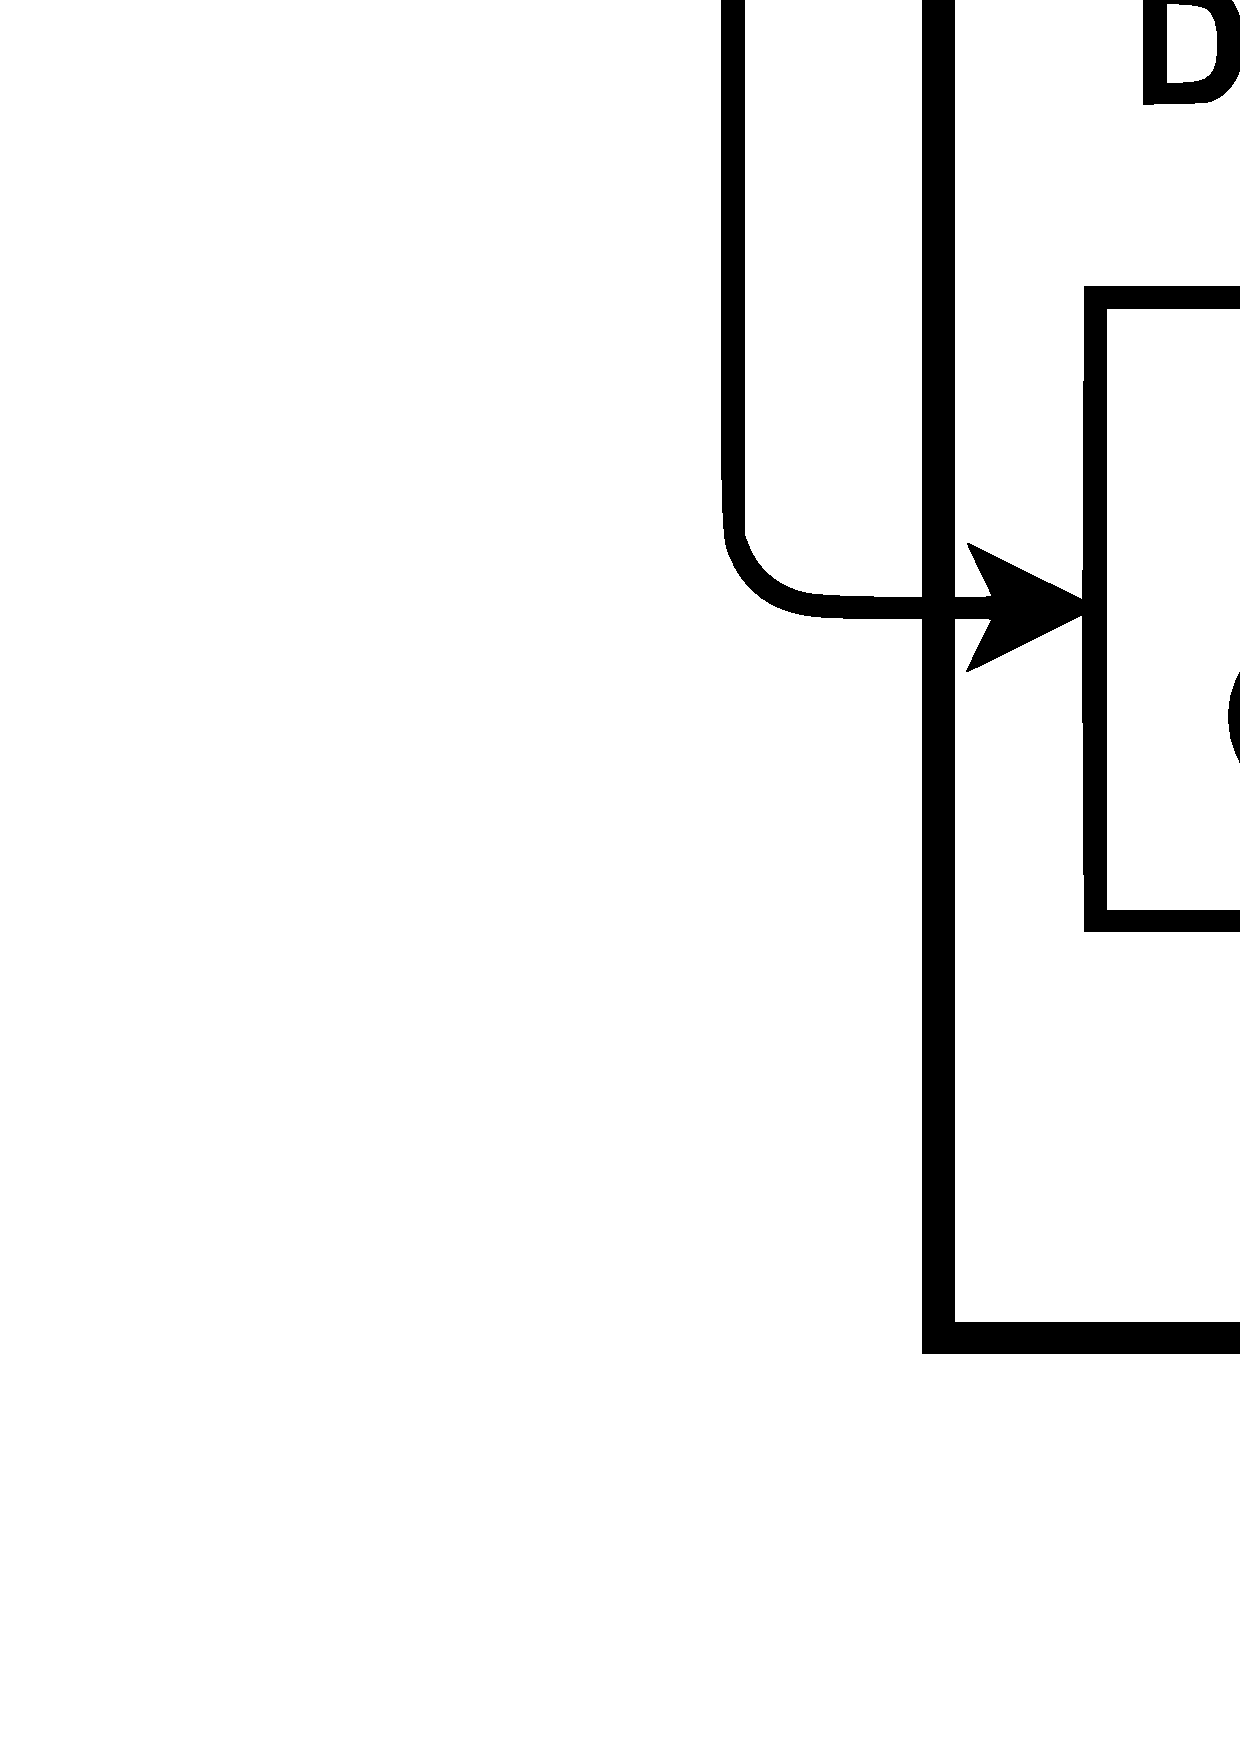
\includegraphics[width=0.8\linewidth]{DeepEncoderDecoder.pdf}
\end{center}
   \caption{Illustration of pixel-shuffled symmetric Encoder-Decoder architecture.}
\label{fig_1}
\end{figure*}
The advantages of our proposed architecture (illustrated in Fig.~\ref{fig_0} and \ref{fig_1}) are fourfold. 
First, the architecture is naturally scalable in the sense that codes can be decoded at more than one compression quality levels, and it allows efficient coding of correlated sources which are not physically co-located. This is especially attractive in video streaming applications \cite{guillemot2007distributed,gehrig2008distributed}. Second, unlike classical DSC which requires customized code design for different scenarios \cite{xiong2004distributed}, data-driven DSC framework can handle nontrivial distribution of image sources with arbitrary correlations. Third, the computation complexity of the encoder can be transferred to the decoder, a system of low complexity encoders can be used in a variety of application domains, such as multi-view video coding \cite{girod2005distributed}, sensor networks \cite{xiong2004distributed}, and under-water image processing where communication bandwidth and computational power are quite restricted \cite{stojanovic2009underwater,schettini2010underwater}. Fourth, the distributed framework can be more robust against heterogeneous noises or malfunctions of encoders, and such robustness can be crucial in, e.g., unreliable sensor networks \cite{girod2005distributed,ishwar2005rate,xiao2006distributed}.

The paper is outlined below. We review previous related work in Section 2 and describe our proposed method in details in Section 3. We describe our architecture for general image compression and its base modules in Section 3.1-3.4. Then we elaborate the Deep Distributed Source Coding framework in Section 3.5. Experimental results are shown in Section 4, followed by conclusions in Section 5.

%------------------------------------------------------------------------
\section{Related Work}
Though there has been a variety of research on lossy data compression in the past few decades, little attention has been paid to a systematic approach for general and practical distributed code design, especially in the presence of an arbitrary number of nontrivial data sources with arbitrary correlation %and possibly sources and correlation with memory. 
\cite{xiong2004distributed}. 
A main motivation of this work is to attempt to replace the practical hand-crafted code design with data-driven approaches. 
To our best knowledge, what we propose is the first data-driven DSC architecture. 
Unlike hand-crafted quantizers, our neural network-based quantizers show that the correlations among different data sources can be trained by the model parameters. We empirically show that the Slepian-Wolf limit can be achieved with our methodology. 

\subsection{Image compression with Deep Learning}
There exist a variety of classical codecs for lossy image compression. Although the JPEG standard \cite{wallace1992jpeg} was developed thirty years ago, it is still the most widely used image compression method. Several extensions to JPEG including JPEG2000 \cite{skodras2001jpeg}, WebP \cite{google2010webp} and BPG \cite{bellard2014bpg} have been developed. Most of these classical codecs rely on a quantization matrix applied to the coefficients of discrete cosine transform or wavelet transform.

The standard methods of compression with deep learning roughly fall into two categories. Non-recurrent autoencoders which rely on $\mathcal{L}_1$ penalty to sparsify the 8-bit integer codes, and recurrent models which introduce binary codes at each iteration. 
%Autoencoders are widely used as a general framework for neural network-based image compression. Bottleneck representations are quantized into 8-bit integers or binaries. 
The compression rate of non-recurrent models is not scalable and their performance heavily rely on the sparsity which entropy codec can take advantage of. 
Another challenge is to well define the derivative of quantizations of bottleneck representations. Ball\'e et al. \cite{balle2016end} replaced non-differentiable quantization step with a continuous relaxation by adding uniform noises. Toderici \cite{toderici2015variable}, on the other hand, used a stochastic form of binarization. 
The recurrent model~\cite{toderici2015variable,johnston2017improved}, on the other hand, has scalable compression rates. It generates more codes when the residual difference between the input and output of the model is compressed again.

\subsection{Distributed Source Coding}

\begin{figure}[t]
\begin{center}
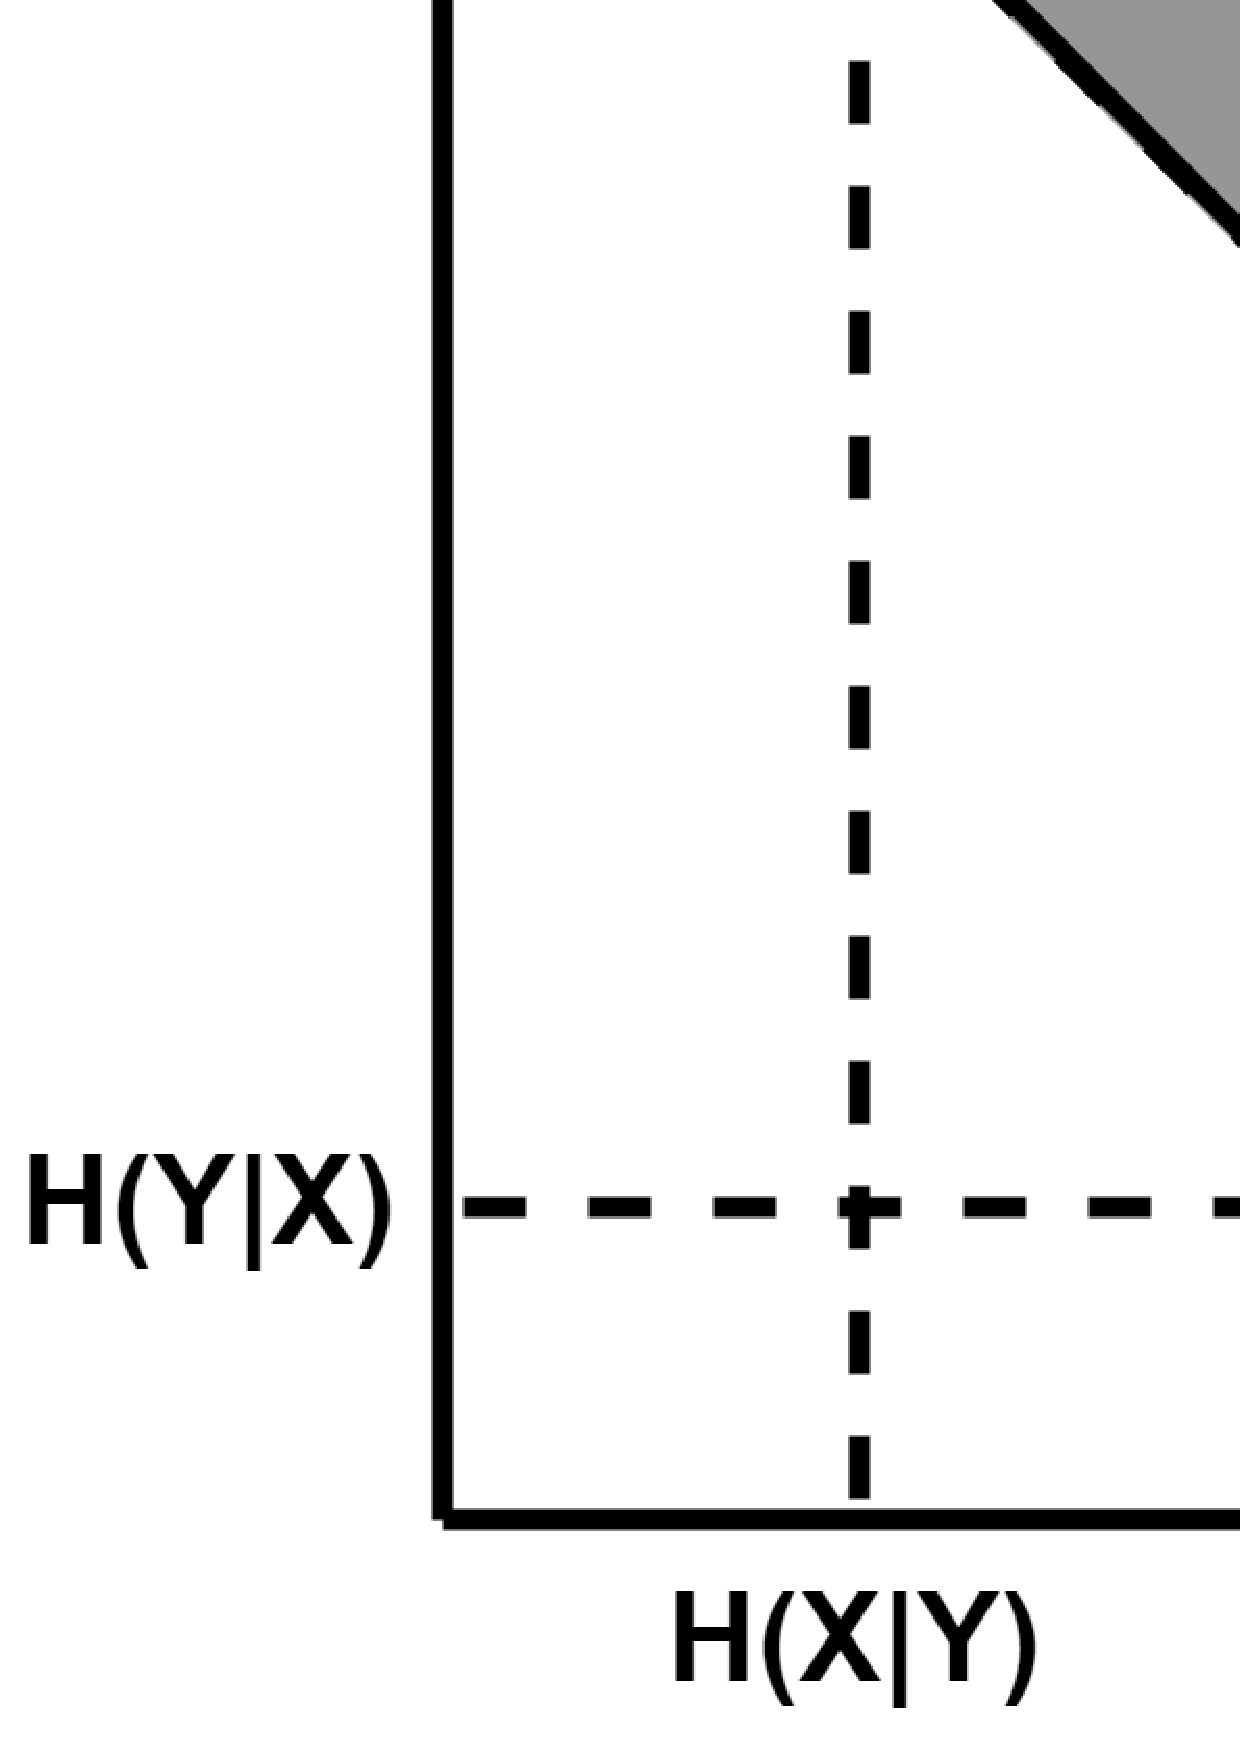
\includegraphics[width=0.8\linewidth]{SlepianWolf.pdf}
\end{center}
   \caption{The Slepian-Wolf achievable region for two sources $X$ and $Y$.}
\label{fig_2}
\end{figure}
Our methodology is deeply rooted in information-theoretic results on DSC which have been established since 1970s. The Slepian-Wolf \cite{slepian1973noiseless} Theorem shows that two correlated data sources encoded separately and decoded jointly can perform as well as joint encoding and decoding, and outperform separate encoding and separate decoding. The striking result indicates that as long as the codes are jointly decoded, there can be no loss in coding efficiency even the codes are separately encoded. Cover \cite{cover1975proof} generalizes the achievability of Slepian-Wolf coding to arbitrary number of correlated sources. Wyner-Ziv Coding \cite{wyner1976rate} gives a rate-distortion curve as an extension to lossy cases.

A classical illustration of Slepian-Wolf achievable region is shown in Fig.~\ref{fig_2}. We can achieve the performance of joint encoding and decoding of two data sources $X$ and $Y$ where the bit rate $R$ is equal to the joint entropy $H(X,Y)$ with separate encoding and joint decoding. Specifically, the achievable region proved by the Slepian-Wolf Theorem is given by $R_X\geq H(X|Y),R_Y\geq H(Y|X),$ and $R_X+R_Y\geq H(X,Y)$ as shown in the shaded area of Fig.~\ref{fig_2}. Here $R_{\cdot},H(\cdot)$ denote the bit rates and (conditional) entropies in classical Shannon theory. In practice, although some works are proposed to approach the mid-point $C$ \cite{schonberg2004distributed}, the most widely used scheme is source coding with side information (syndrome bits) at the decoder \cite{pradhan2003distributed}. This code design takes advantage of the corner points $A$ and $B$ which correspond to $R(X,Y) = R(Y)+R(X|Y)$ and $R(X,Y) = R(X)+R(Y|X)$ respectively. As an example, two 8-bit grayscale images $X$ and $Y$ have pixel values at the same location with (nonlinear) correlation implicitly determined by $x \in \{y-4, y-3, y-2, y-1, y, y+1, y+2, y+3\}$. Instead of sending 16 bits, we can send bits with $R=H(Y)+H(X|Y)$. We can take modulo of $x-y$ with respect to $8$ which only requires a 3-bit codebook $\tilde{x} \in \{4, 5, 6, 7, 0, 1, 2, 3\}$. Specifically, for $x=124$ and $y=128$, we transmit $\tilde{x}=(x-y) \mod 8$ which is 4 and $y=128$. The joint decoder will decode $x$ based on $y$ as $x = y-4 = 124$.

Some researchers have also shown the applicability of DSC on still images \cite{dikici2005distributed}. In practical applications, low complexity video encoding benefits from the DSC framework which can transfer the complexity of encoder to decoder \cite{puri2002prism,aaron2002wyner}. Scalable Video Coding can also be incorporated with DSC \cite{xu2006layered}. These proposed methods indicate the feasibility of DSC in our problem setting.

%-------------------------------------------------------------------------
\section{Methods}
In this section, we first describe the symmetric Encoder-Decoder architecture used in our research work. We will elaborate the base modules including Convolutional Long short-term memory (ConvLSTM), Pixel (Un)Shuffle, and Binarizer used in our model. We will then describe how this Deep Learning architecture is used in Distributed Source Coding framework.

\subsection{Network Architecture}
Our compression network consists of an encoder, a binarizer, and a decoder. The activation function following each Convolutional Neural Network (CNN) module is $\tanh$. For the first iteration of our model, the input images are initially encoded and transformed into $(-1,1)$ by $\tanh$ activation function. Binary codes are quantized from transformed bottleneck representations. The decoder then reconstructs images based on the received binary codes. Finally, we compute the residual difference between the original input images and the reconstructed output images. At the next iteration, the residual difference is feedback as the new input for our model. This procedure is repeated multiple iterations to gain more codes for better reconstruction performance. Therefore, the reconstructed images at each iteration are the sum of output reconstructions from previous and current iterations.

Consider dataset $X = \{x\}^{N}$ consisting of $N$ i.i.d. samples of some continuous or discrete variables $x$. The data generating process is unknown. Autoencoders for compression and reconstruction can be formulated in the following way. Data can be compressed with a neural network-based encoder $f(x;\theta)$ into quantized codes $\tilde{z}$ and reconstructed with a decoder $g(\tilde{z};\phi)$. We can binarize bottleneck representations $z$ and control the compression quality by varying its channel sizes. The loss function $\mathcal{L}(x,\tilde{x})$ is minimized with respect to the model parameters $\theta$ and $\phi$.
\begin{align}
z &= f(x;\theta),\\
\tilde{z} &= \text{Binarize}(z),\\
\tilde{x} &= g(\tilde{z};\phi),\\
\text{Minimize } \mathcal{L}&(x,\tilde{x})
\end{align}
Deep recurrent autoencoder gradually increases compression quality by creating a correlated residual sequence from the difference between the input and output of our model. The advantage of recurrent model is that we can train one model with scalable compression quality. Classical autoencoders, on the contrary, have to train multiple networks with different penalty coefficients or channel sizes for different compression qualities. Suppose $T$ iterations are used, we can formulate the recurrent autoencoder in the following way.
\begin{align}
z_t &= f(x_t;\theta),\\
\tilde{z}_t &= \text{Binarize}(z_t),\\
\tilde{x}_t &= g(\tilde{z}_t;\phi),\\
x_{t+1} &= x_t-\tilde{x}_t\text{, }\tilde{x}_1=0,\\
\text{Minimize } \frac{1}{T}&\sum_{t=1}^{T}\mathcal{L}(x_1,\sum_{i=1}^{t}\tilde{x}_i).
\end{align}
In the recurrent autoencoder, the compression quality is controlled by several factors including the scale factor of Pixel (Un)Shuffle module $r$, the depth of model $D$, the channel size of bottleneck representations $C$, and the number of iterations $T$. The height and width of bottleneck representations are determined by $T$ and $D$. As we have $N$ batch images with shape $H,W$, the size of codes after $T$ iterations is $(N,T,C,H/(r^D),W/(r^D))$. For example, with $r=2$, $D=3$, and $C=2^D$, one $32 \times 32$ RGB image will generate $(1,1,8,4,4)$ binary codes for a single iteration. Thus, we will add up $\frac{8
\times4\times4}{32\times32} = 0.125$ Bit Per Pixel (BPP) for this iteration. Although we configure these hyper-parameters, we believe it is possible to train these configurations in future works.

\subsection{Convolutional Long short-term memory}
As proposed by \cite{xingjian2015convolutional}, simply replacing the Fully Connected (FC) layer in LSTM with convolutional layer, ConvLSTM is able to capture spatial structure in the temporal sequence. We do not add any bias term to our modules because the output of each layer is saturated by $\tanh$. The key equations are shown below.
\begin{align}
i_t &= \sigma(W_{xi}*x_t + W_{hi}*h_{t-1}) ,\\
f_t &= \sigma(W_{xf}*x_t + W_{hf}*h_{t-1}) ,\\
c_t &= f_tc_{t-1}+i_t\tanh(W_{xc}*x_t + W_{hc}*h_{t-1}), \\
o_t &= \sigma(W_{xo}*x_t + W_{ho}*h_{t-1}) ,\\
h_t &= o_t\tanh(c_t).
\end{align}
The first and last layers of the encoder and decoder are feed-forward Convolutional Neural Network with $\tanh$ activations. The recurrent layers are all ConvLSTM networks. We do not replace CNN layer with ConvLSTM because the size of the feature maps of hidden state at shallow layers cost a mass amount of memory. From our various experimental studies, the performance does not degrade significantly either because no convolutional layers are in between ConvLSTM layers.

\subsection{Pixel (Un)Shuffle}
We resize feature maps with Pixel (Un)Shuffle modules. Pixel Shuffle module is originally proposed by \cite{shi2016real} to tackle image and video super-resolution problem. Compared to bilinear interpolation and tranposed convolutional layers, Pixel Shuffle module is much more computationally efficient, because it is non-parametric and only requires tensor reshaping and dimension permutation. We note that although this method is widely used for upscaling, it is actually invertible and we propose to use its inversion for downscaling. Thus, the encoder and decoder can be constructed symmetrically. Our experimental results show that symmetric Encoder-Decoder architecture actually produces much better results with less number of parameters, compared to the asymmetric architecture as proposed in \cite{toderici2017full}. We describe these two modules with the following pseudocodes \ref{alg_0} and \ref{alg_1}.

\begin{algorithm}
\caption{Pixel UnShuffle}
\begin{algorithmic}
\label{alg_0}
\REQUIRE $X\sim(N,C,H,W)$, $r_H,r_W$
\ENSURE $r_H,r_W$ are integers, divides $H,W$
\STATE Reshape $X\sim(N,C,H/r_H,r_H,W/r_W,r_W)$
\STATE Permute $X\sim(N,C,r_H,r_W,H/r_H,W/r_W)$
\STATE Reshape $X\sim(N,C\times r_H\times r_W,H/r_H,W/r_W)$
\end{algorithmic}
\end{algorithm}

\begin{algorithm}
\caption{Pixel Shuffle}
\begin{algorithmic}
\label{alg_1}
\REQUIRE $X\sim(N,C,H,W)$, $r_H,r_W$
\ENSURE $r_H,r_W$ are integers, $r_H\times r_W$ divides $C$
\STATE Reshape $X\sim(N,C/(r_H \times r_W),r_H,r_W,H,W)$
\STATE Permute $X\sim(N,C/(r_H \times r_W),H,r_H,W,r_W)$
\STATE Reshape $X\sim(N,C/(r_H \times r_W),H \times r_H,W \times r_W)$
\end{algorithmic}
\end{algorithm}

\subsection{Binarizer}
The derivative of quantization function is only defined at the rounded integer itself. Therefore, we have to replace its derivative in the backward pass of backpropagation with a form of smooth approximation \cite{rumelhart1988learning}. Thanks to a thorough discussion of different alternative approaches by \cite{theis2017lossy}, we choose to use identity function to replace its derivatives that cannot be well defined as shown in \ref{eq_15}. During training, we use a stochastic form of binarization proposed by \cite{toderici2017full}. For bottleneck representations $z \in (-1,1)$, the details of binarizer $\tilde{z}=\text{Binarize}(z)$ are described as follows, where $W_{\cdot}$ denote the standard parameter matrices between two network layers.
\begin{align}
\intertext{\textbf{Train}}
\tilde{z}=\text{Binarize}(z) &= 
    \begin{cases}
      1, &  \text{with probability } (z+1)/2\\
      -1, & \text{otherwise}
      \end{cases} \nonumber \\
\frac{d}{dz}\tilde{z} &:= \frac{d}{dz}\mathbb{E} (\tilde{z}) =  \frac{d}{dz}\mathbb{E} (z) = 1\label{eq_15}
\intertext{\textbf{Test}}
\text{Binarize}(z) &= 
    \begin{cases}
      1, & \text{if } z\geq0 \\
      -1, & \text{otherwise}
      \end{cases}
\end{align}

\subsection{Deep Distributed Source Coding Framework}
Fig.~\ref{fig_0} and \ref{fig_1} illustrates our Deep DSC coding framework. Similar to classical DSC framework, each data source is encoded separately and decoded jointly. Traditionally, researchers have to design different kind of codes for specific scenarios \cite{schonberg2004distributed}. We propose to use data-driven approach to handle complex scenarios where the distribution of data sources are unknown and their correlations can be arbitrary. Our proposal may also shed new light on sophisticated application scenarios such as videos where data sources and correlations are time dependent.

In our neural network-based DSC, %the whole encoding and decoding procedure are trained jointly. 
$M$ distributed encoders encode corresponding data sources $x^m$ that can be arbitrarily correlated. Each neural network-based encoder $f(x^m;\theta^m)$ has their own model parameters $\theta^m$. After binarizing bottleneck representations $z^m$, code sources $\tilde{z}^m$ are transmitted and concatenated batch-wisely. A single decoder $g(\tilde{z}^m;\phi)$ reconstructs images $\tilde{x}^m$ from all sources with the same model parameters $\phi$. 
In particular, the parameters of the following model are optimized with backward propagation \cite{rumelhart1988learning}. 
\begin{align}
z_t^m &= f(x_t^m;\theta^m),\\
\tilde{z}_t^m &= \text{Binarize}(z_t^m),\\
\tilde{x}_t^{m} &= g(\tilde{z}_t^{m};\bm{\phi}),\\
x_{t+1}^{m} &= x_t^{m}-\tilde{x}_t^{m}\text{, }\tilde{x}_1^{m}=0,
\end{align}
\begin{align}
\text{Minimize } \frac{1}{MT}&\sum_{t=1}^{T}\sum_{m=1}^{M}\mathcal{L}(x_1^m,\sum_{i=1}^{t}\tilde{x}_i^m).
\end{align}
Our result shows that the resulting distributed model can perform as well as encoding all data by one single encoder. However, if we encode and decode each data source separately, the performance becomes significantly worse. Moreover, correlations among data sources cannot be learned with separate parameters of decoders, i.e. with 
$\tilde{x}_t^{m} = g(\tilde{z}_t^{m};\bm{\phi^m})$.
%------------------------------------------------------------------------
\section{Experiments}
We use MNIST dataset \cite{lecun1998gradient} consisting of 60,000 training and 10,000 testing grayscale handwritten digit images. The digits have been resized from $28 \times 28$ to $32 \times 32$. The Adam optimizer \cite{kingma2014adam} is used with $\epsilon = 1e-8$, $\beta_1 = 0.9$ and $\beta_2 = 0.999$. We train model with $\mathcal{L}_1$ loss, batch size $N=100$ and learning rate $0.001$ for a total of 200 epochs. We start to decay learning rate by half at the 70th epoch and at every 20 epochs thereafter.

As described in section 3.1, we set the scaling factor for Pixel (Un)Shuffle module to be $r=2$, depth of model $D=3$, and code channel size $C=2^D$. For $T=16$, one minibatch of grayscale images with shape $(100,1,32,32)$ will be encoded to be a $(100,16,8,4,4)$ binary tensor. We evaluate all models with the metric Peak Signal to Noise Ratio (PSNR) against the Bit Per Pixel (BPP).

\begin{figure}[t]
\begin{center}
\includegraphics[width=0.8\linewidth]{codec.pdf}
\end{center}
	\vspace{-0.2cm}
   \caption{Our symmetric pixel-shuffled Encoder-Decoder outperforms classical codecs and baseline neural network-based codecs.}
   \vspace{-0.2cm}
\label{fig_3}
\end{figure}

We compare our model to the baseline model \cite{toderici2017full} and classical codecs like JPEG~\cite{wallace1992jpeg}, JPEG2000~\cite{skodras2001jpeg} and BPG~\cite{bellard2014bpg}. To directly compare the performance of network architecture, we ignore some techniques introduced by \cite{toderici2017full} and \cite{johnston2017improved} such as progressive entropy coding and hidden-state priming. Instead of bilinear interpolation or convolutional layers used in previous works\cite{toderici2017full,theis2017lossy,johnston2017improved}, our network architecture uses Pixel Shuffle in the Encoder. As a result, our network architecture has a symmetric Encoder-Decoder structure and also few number of parameters. Fig.~\ref{fig_3} shows that our symmetric pixel-shuffled Encoder-Decoder architecture outperforms classical codecs and baseline neural network-based codecs.

We run experiments with $(2,4,8,10)$ number of distributed sources. Each encoder encodes data from each data source without communicating with other encoders. The decoder jointly decodes the codes gathered from each distributed encoder. First, we compare our result, labeled as \textit{Distributed}, to the case where all data are trained with one encoder and one decoder jointly, labeled as \textit{Joint}. The `Joint' curve is approximated as the theoretical upper bound of performance. %theoretical upper bound $H(X,Y)$. 
Second, we compare our result to the case where each data source is trained with a separate pair of encoder and decoder, labeled as \textit{Separate}. We test each distributed encoder separately with all test data. The solid curves are the average performance across all encoders. At each iteration, the confidence band is determined by the best and worst performance of all encoders. 

Our experimental studies in the following sections consist of three aspects. We first experiment data sources with different correlations. We then show the performance of low complexity encoders which are trained with less number of iterations. Finally, we show the robustness of our distributed framework in the absence of a number of distributed sources.

\begin{figure*}
\begin{center}
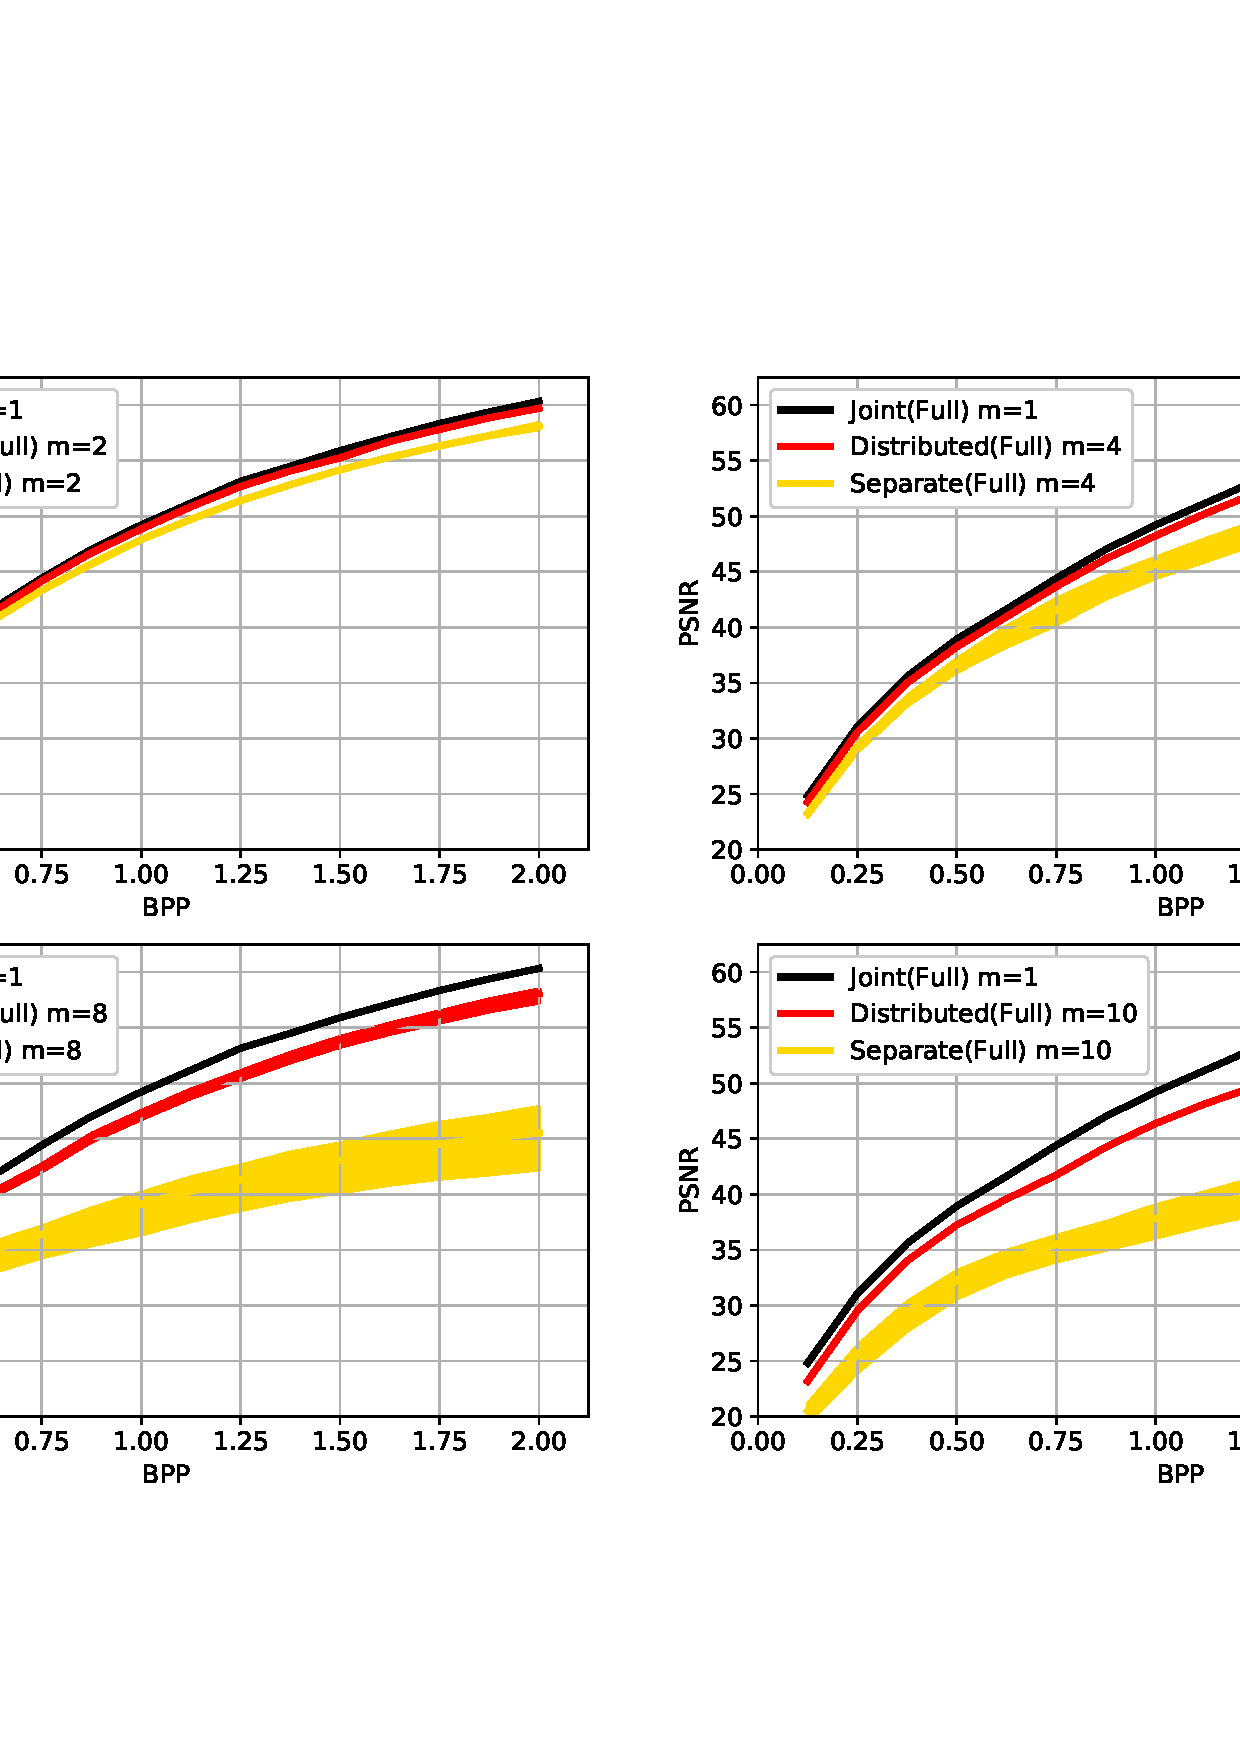
\includegraphics[width=0.8\linewidth]{full_subset_band.png}
\end{center}
	\vspace{-0.2cm}
   \caption{Rate-distortion curves for data sources distributed by random subsets with $T=16$ for all sources.}
   \vspace{-0.2cm}
\label{fig_4}
\end{figure*}

\begin{figure*}
\begin{center}
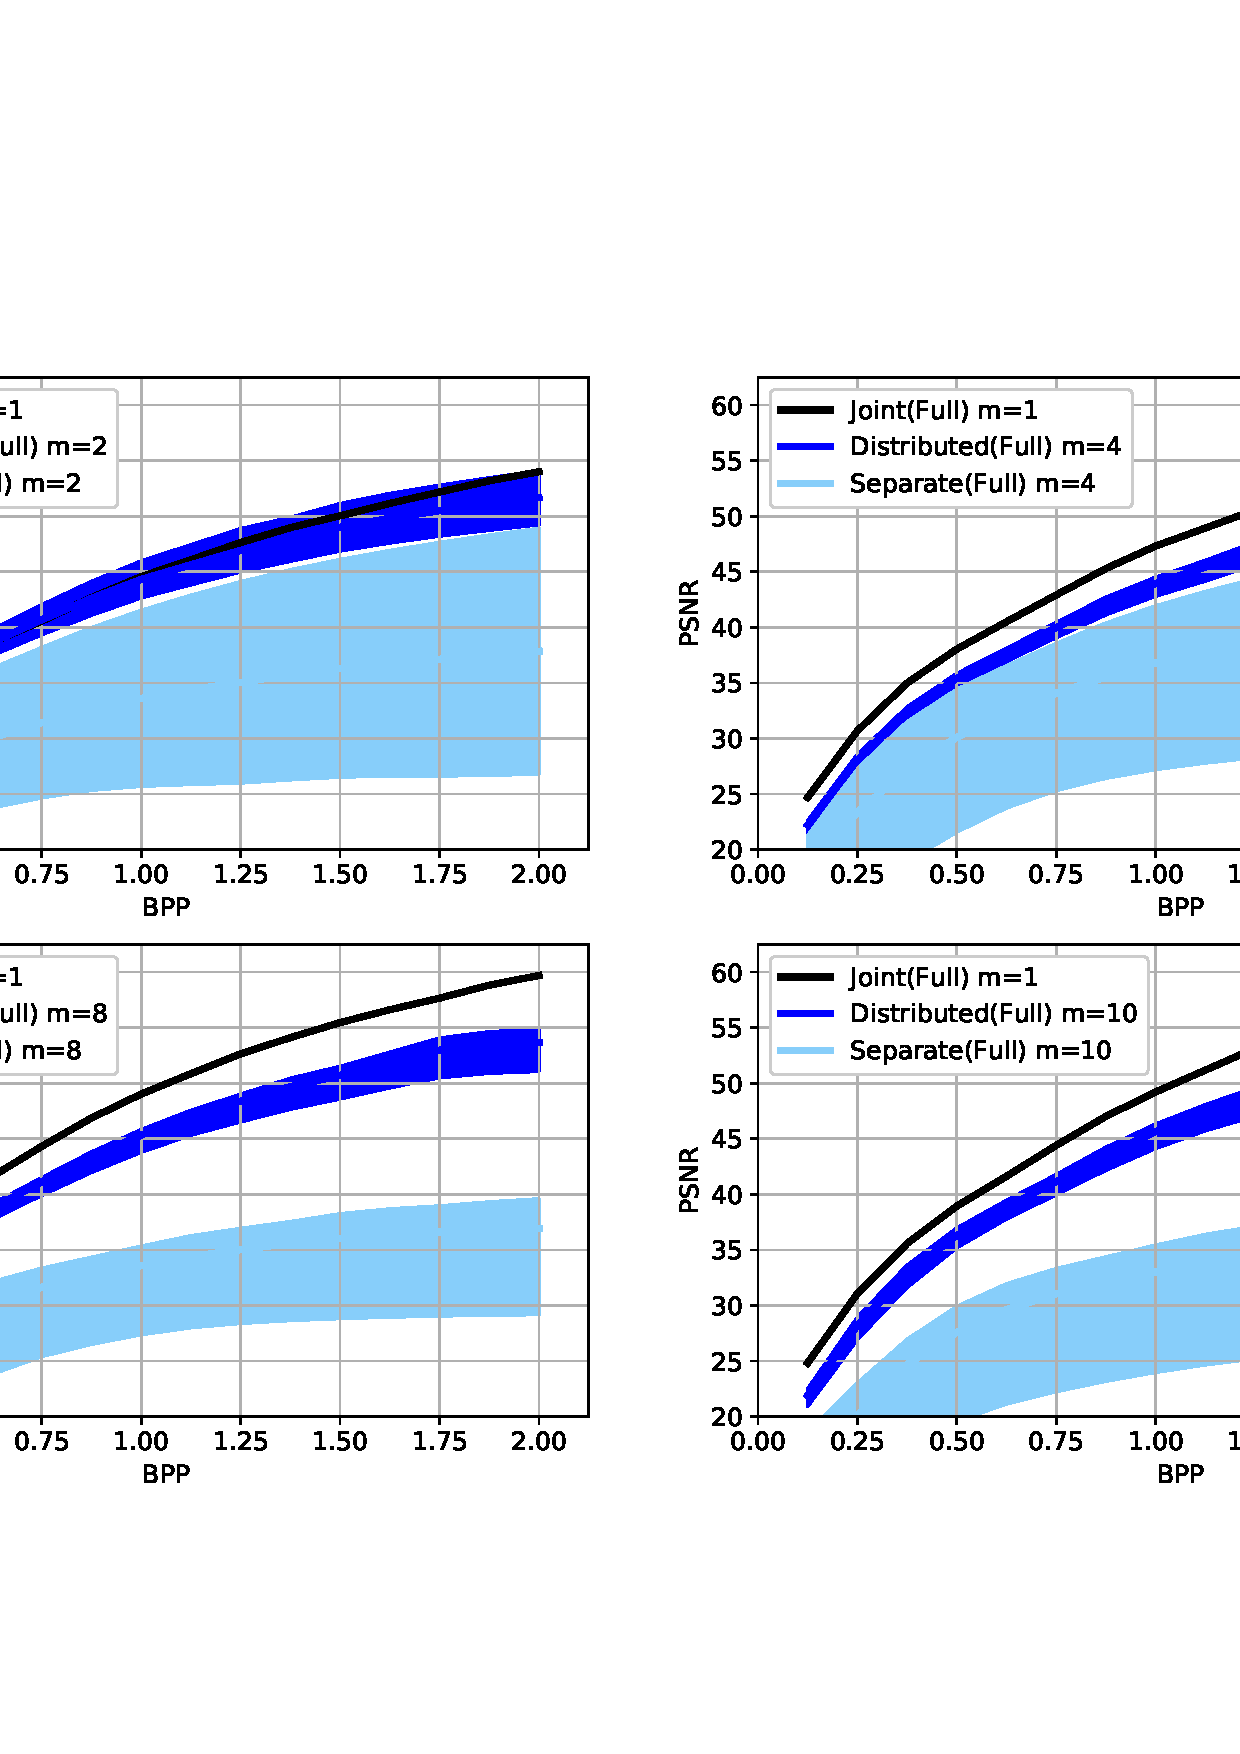
\includegraphics[width=0.8\linewidth]{full_class_band.png}
\end{center}
	\vspace{-0.2cm}
   \caption{Rate-distortion curves for data sources distributed by class labels with $T=16$ for all sources.}
   \vspace{-0.2cm}
\label{fig_5}
\end{figure*}

\begin{figure*}
\begin{center}
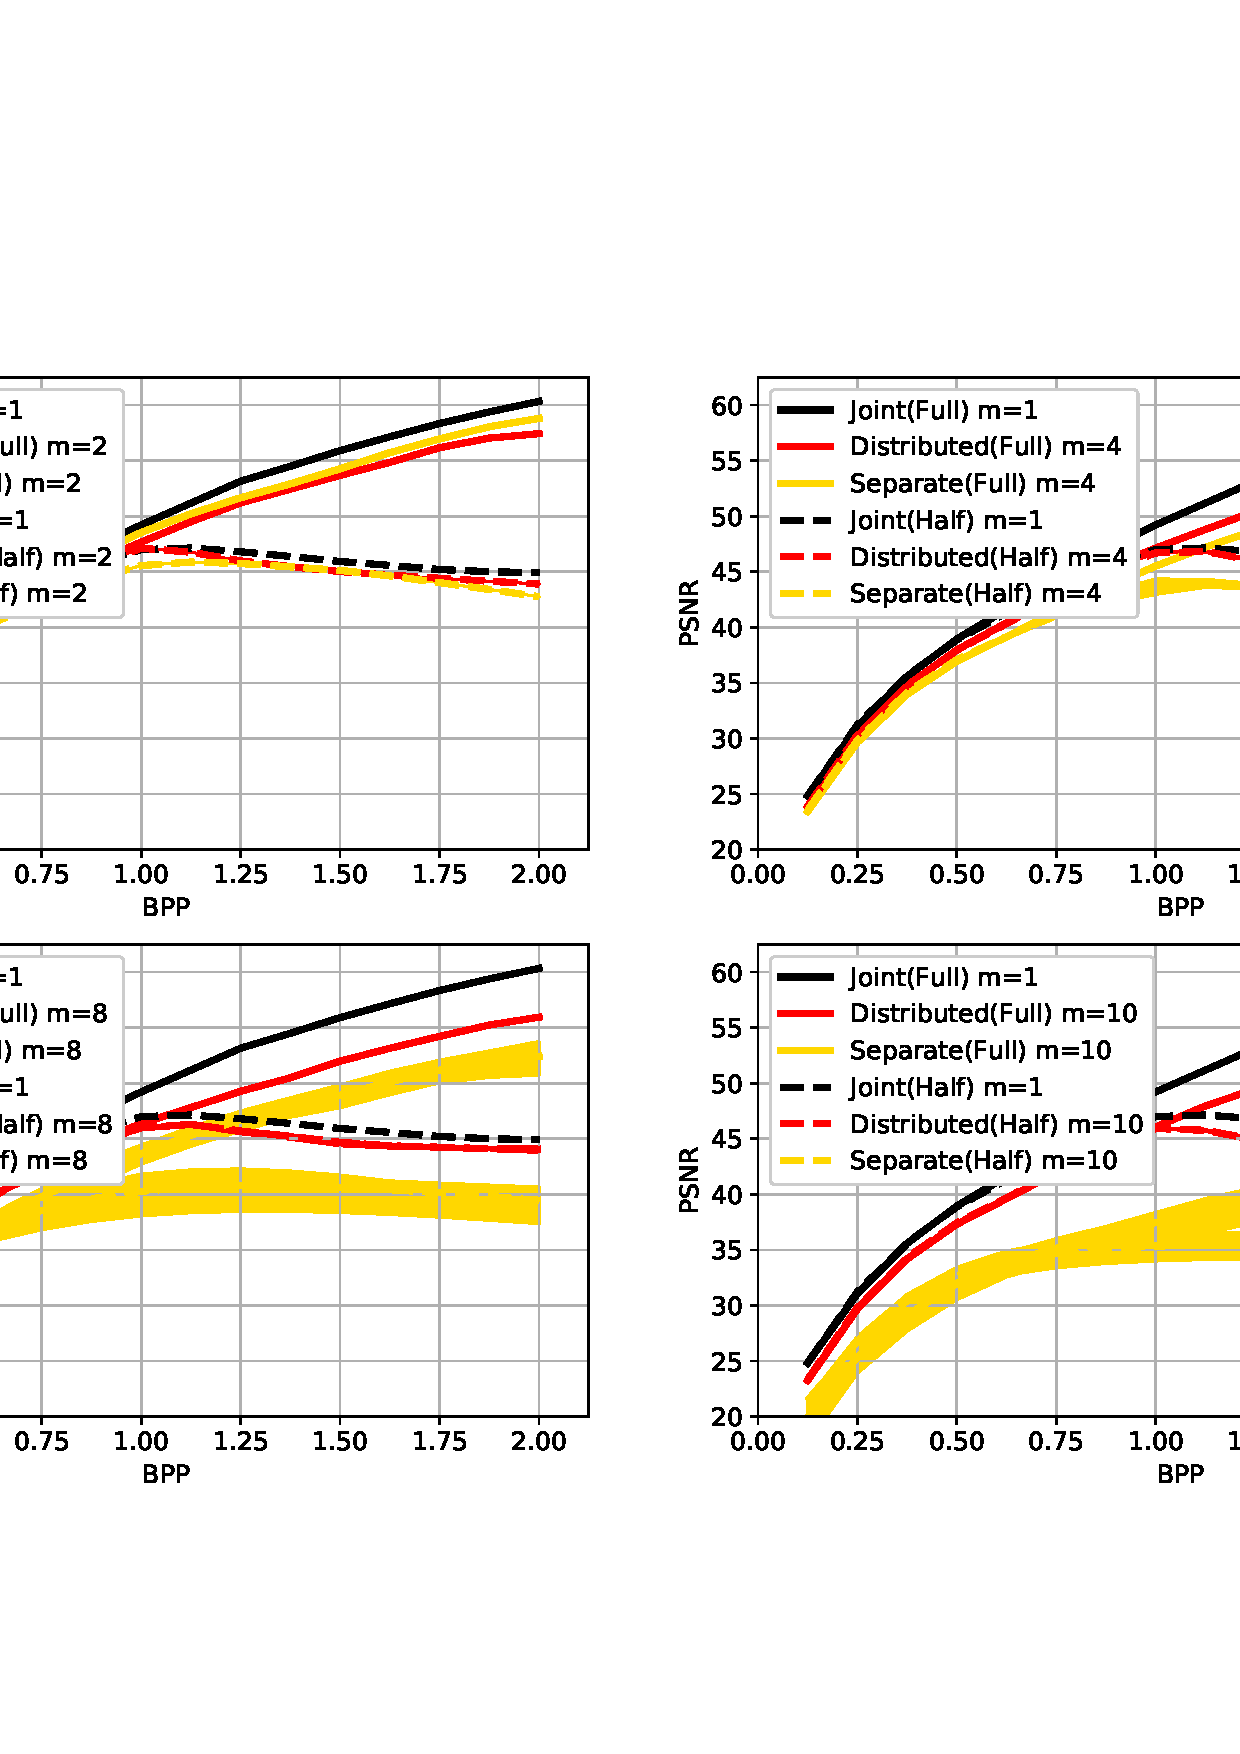
\includegraphics[width=0.8\linewidth]{half_subset_band.png}
\end{center}
	\vspace{-0.2cm}
   \caption{Rate-distortion curves for data sources distributed by random subsets with $T=16$ for the first half of sources and $T=8$ for the second half of sources.}
   \vspace{-0.2cm}
\label{fig_6}
\end{figure*}

\begin{figure*}
\begin{center}
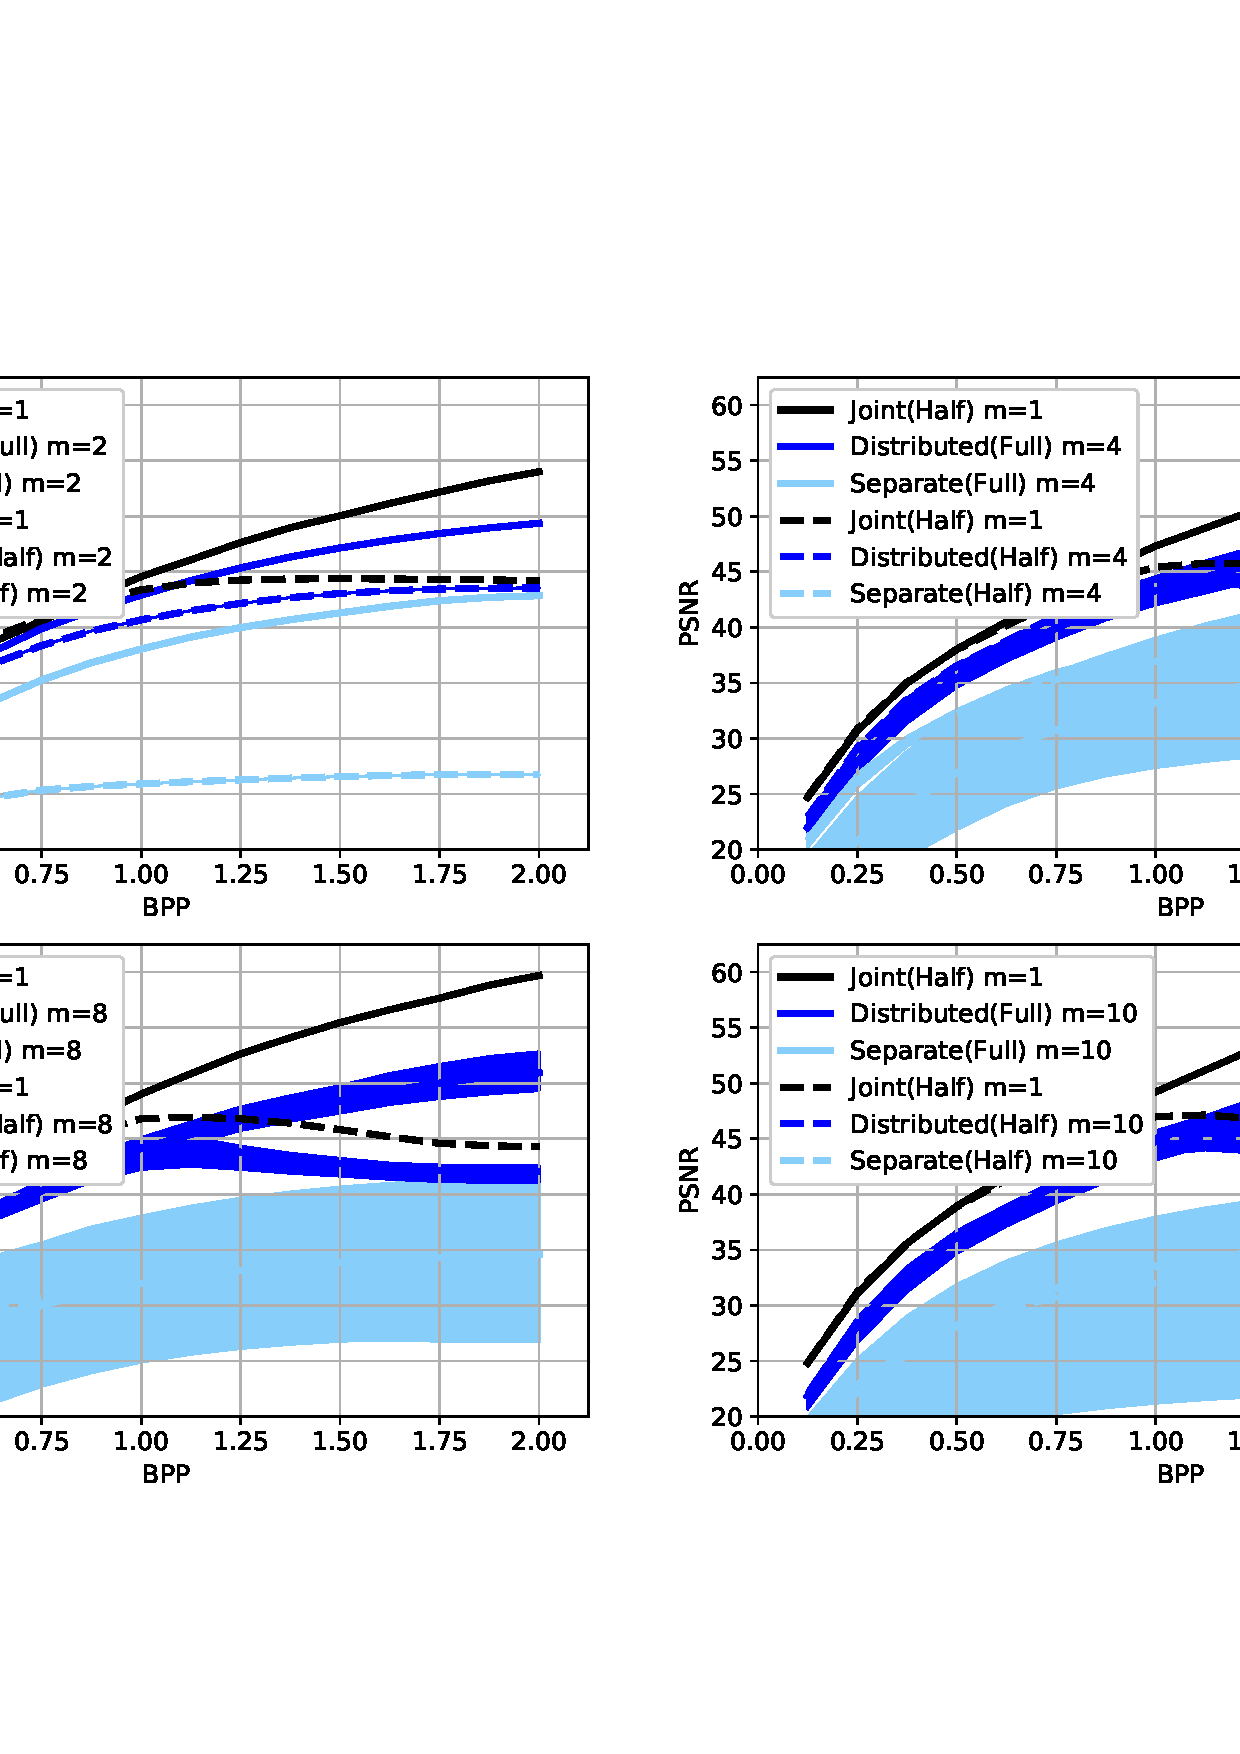
\includegraphics[width=0.8\linewidth]{half_class_band.png}
\end{center}
	\vspace{-0.2cm}
   \caption{Rate-distortion curves for data sources distributed by class labels with $T=16$ for the first half of sources and $T=8$ for the second half of sources.}
   \vspace{-0.2cm}
\label{fig_7}
\end{figure*}

\subsection{Arbitrary Correlated Sources}
To address the advantage of our DNN-based DSC framework, we first experiment distributed sources with different correlations. The distributed encoders are indexed as $1, \ldots, m$. We split data into random subsets and also split them by class labels. We show the result of data sources distributed by random subsets in Fig.~\ref{fig_4}, \ref{fig_6} and by class labels in Fig.~\ref{fig_5}, \ref{fig_7}. In the first case, each distributed encoder is trained with a subset of data and only the decoder can access the codes compressed from each data source. In the second case, we distribute data sources by class labels. For example, the $m$th encoder can only access data of digit $m-1$ and the label is $m-1$ ($m\leq 10$). %The theoretical limit in the case of $m<10$ is also obtained with data of digits with labels $<m$.

The curve of distributed encoders shows that the performance of training distributed encoders and joint decoder can be very close to the theoretical limit. As the number of encoders grows, the performance decreases a little, but still dominantly outperforms training codecs for each data source separately. From various experiments we found that the gap will become smaller when more data are available. The gap also diverges as more bits are generated. This is because the residual differences used as input at each iteration are less correlated among data sources than the original images. This experiment clearly shows that near-oracle performance can be achieved without specifically estimating the correlations among different sources, a desirable feature not enjoyed by classical DSC code design. The results show that our Deep DSC framework is able to adaptively learn arbitrary correlations among arbitrary number of data sources. 

\subsection{Low Complexity Encoding}
We also demonstrate the performance of low complexity encoders which are trained with less number of iterations. In this experiment, the first half of encoders are trained with $16$ iterations, labeled as \textit{Full}, and the second half of encoders are only trained with $8$ iterations, labeled as \textit{Half}. For example, for $m=8$, encoders $1$ to $4$ are trained with 16 iterations while encoders $5$ to $8$ are trained with 8 iterations. In Fig.~\ref{fig_6} and Fig.~\ref{fig_7}, we show the dashed lines for $T=8$ and solid lines for $T=16$ respectively. The theoretical limits (in black lines) are trained with all available data. The first half of encoders and the second half of encoders only access half of the whole dataset respectively.

Although the theoretical limits are obtained from all data, full and half complexity encoders %, only using half of the whole dataset, 
can still approach their theoretical limits (in black dash). Half complexity encoders perform as well as full complexity encoders in the first 8 iterations, because their correlations of the first eight iterations are trained properly with the model parameters. After the eighth iteration, both full and half complexity encoders can still approach their theoretical limits, because the trained correlations of residual differences from the first eight iterations can be reused at the second eight iterations without training. However, without specifically training the correlations after the eighth iterations, the performance of half complexity encoders slightly decreases when BPP is larger than 1. %a little compared to Fig.~\ref{fig_4} and \ref{fig_5}.


\subsection{Robust Distributed Encoding}
Our data-driven DSC framework, unlike classical DSC code design, does not require synchronization of data sources. In classical DSC code design, if syndrome bits $H(X|Y)$ are used and the data source $X$ is accidentally blocked, we will not be able to decode data source $Y$. As mentioned previously, we test each encoder separately with all test data once training is finished. Even only one of distributed encoders is functional, it can still benefits from its correlations with other sources because their correlations are already trained with the model parameters. 

%Our results are summarized 
%A confidence band is determined by the best and worst performance of all encoders at each iteration.
All our experiments show that distributed encoders not only dominates separately trained codecs but also have narrower confidence band. As the number of encoders increases, the confidence band of separately trained codecs becomes wider because each separate codec can only access very limited amount of data and thus suffer from overfitting. As the number of iterations increases, the confidence band also becomes wider. This is because the residual differences at later iterations become less correlated. Finally, the confidence band of data sources distributed by class labels is also wider than that of data sources distributed by random subsets. This is mainly because encoders specialize on data with the same label so their performance fluctuates more than encoders trained by data sources distributed by random subsets. %; 2 part of data sources distributed by class labels when $m<10$.
%------------------------------------------------------------------------
\section{Conclusion}
We introduce a data-driven Distributed Source Coding framework based on Deep Recurrent models. Compared to classical code design, our method has the following advantages. First, the compression quality of our recurrent model is scalable. Data sources can be efficiently compressed at different bit rates with a single recurrent model. Second, instead of explicitly estimating the correlations among data sources in advance, we use data-driven approach to learn the correlations with the neural network parameters. Therefore, given enough training data, our method can handle arbitrary number of sources with arbitrary correlations. Third, as one of the most important applications of Distributed Source Coding, low complexity encoder is also shown to be feasible based on our experimental results. Data sources trained with less data and fewer number of iterations can still approach the theoretical limit obtained when all data are used. Finally, we show the robustness of our framework. Unlike classical code design which may require careful data source synchronization, each distributed encoder of our model, once trained and deployed, can be used independently of others because the correlations are already learned by the model parameters. 

We point out two interesting directions of future work. First, training of the current architecture may be improved by introducing adaptive weights over different iterations, e.g. by using an attention mechanism. Second, the network architecture may be further extended to handle time-dependent data sources.
%We hope this work can pave a new way of practical distributed source code design.
\section*{Acknowledgement}
This work is supported by Office of Naval Research (ONR) grant numbers N00014-18-1-2244.
%------------------------------------------------------------------------
{%\small
\balance
\bibliographystyle{IEEEtran}
\documentclass[10pt,twocolumn,letterpaper]{article}

\usepackage{iccv}
\usepackage{times}
\usepackage{epsfig}
\usepackage{graphicx}
\usepackage{amsmath}
\usepackage{amssymb}
\usepackage{algorithm}
\usepackage{algorithmic}
\usepackage{balance}

% Include other packages here, before hyperref.
\usepackage{bm}

% If you comment hyperref and then uncomment it, you should delete
% egpaper.aux before re-running latex.  (Or just hit 'q' on the first latex
% run, let it finish, and you should be clear).
\usepackage[pagebackref=true,breaklinks=true,letterpaper=true,colorlinks,bookmarks=false]{hyperref}

\iccvfinalcopy % *** Uncomment this line for the final submission

\def\iccvPaperID{4386} % *** Enter the ICCV Paper ID here
\def\httilde{\mbox{\tt\raisebox{-.5ex}{\symbol{126}}}}

% Pages are numbered in submission mode, and unnumbered in camera-ready
\ificcvfinal\pagestyle{empty}\fi
\begin{document}

%%%%%%%%% TITLE
\title{Distributed Lossy Image Compression with Recurrent Networks}

\author{Enmao Diao\\
Duke University\\
{\tt\small enmao.diao@duke.edu}
% For a paper whose authors are all at the same institution,
% omit the following lines up until the closing ``}''.
% Additional authors and addresses can be added with ``\and'',
% just like the second author.
% To save space, use either the email address or home page, not both
\and
Jie Ding\\
University of Minnesota\\
{\tt\small dingj@umn.edu}
\and
Vahid Tarokh\\
Duke University\\
{\tt\small vahid.tarokh@duke.edu}
}

\maketitle
%\thispagestyle{empty}


%%%%%%%%% ABSTRACT
\begin{abstract}
We propose a new architecture for distributed image compression from a group of distributed data sources. The proposed architecture, which we refer to as symmetric Encoder-Decoder Convolutional Recurrent Neural Network, is able to significantly outperform the state-of-the-art compression techniques such as JPEG on rate-distortion curves. We also show that by training distributed encoders and joint decoders on correlated data sources, the performance of compression is much better than that by training codecs separately. For $10$ distributed sources, our distributed system remarkably performs within 2 dB peak signal-to-noise ratio (PSNR) of that of a single codec trained with all data sources. We experiment distributed sources with different correlations and show how our methodology well matches the Slepian-Wolf Theorem in Distributed Source Coding (DSC). Our method is also shown to be robust to the lack of presence of encoded data from a number of distributed sources. To the best of our knowledge, this is the first data-driven DSC framework for general distributed code design with Deep Learning.

\end{abstract}

%%%%%%%%% BODY TEXT
\section{Introduction}
It has been shown by a variety of previous works that Deep Neural Networks (DNN) can achieve comparable results as classical image compression techniques \cite{toderici2015variable,balle2016end,gregor2016towards,toderici2017full,theis2017lossy,johnston2017improved,liu2018cnn}. Most of these methods are based on autoencoder networks and quantization of bottleneck representations, e.g. by quantizing the codes into 8 bit integers and minimizing $\mathcal{L}_1$-penalized loss to sparsify the codes. These models usually rely on entropy codec to compress the sparsified codes. Moreover, to achieve different compression rates, it is unavoidable to train multiple models with different regularization parameters separately.

Among the existing literature of image compression, the recurrent neural network (RNN) based architecture \cite{toderici2015variable} is known to be the pioneering architecture that outperforms classical codecs. The model uses a recurrent autoencoder to encodes the residual difference between the original input and the reconstruction output. At each iteration, new binary coded information is extracted from the residual and the context from previous iterations is stored in the hidden state of the recurrent model. The compression rate, in this case, is varying according to the number of iterations of a single recurrent model. An improved architecture was proposed in \cite{johnston2017improved} that can simultaneously archive spatially adaptive bit rates in a single training phase. 

Motivated by various issues such as data privacy, computational cost, robustness against missing data, the following question has recently gained a lot of research interest. 

\textit{Can distributed encoders perform as well as a single encoder trained with all data sources together?} 

A positive answer from theoretical perspective was given in the context of Distributed Source Coding (DSC). 
In information theory, DSC is an important problem regarding the compression of multiple correlated data sources. The Slepian-Wolf Theorem shows that lossless coding of two or more correlated data sources with separate encoders and a joint decoder can compress data as efficiently as the optimal coding using a joint encoder and decoder \cite{slepian1973noiseless,cover1975proof}. The extension to lossy compression with Gaussian data sources was proposed as Wyner-Ziv Theorem \cite{wyner1976rate}. Although these theorems were published in 1970s, it was after about 30 years that practical applications such as Distributed Source Coding Using Syndromes (DISCUS) emerged \cite{pradhan2003distributed}. One of the main advantages of DSC is that the computation complexity of the encoder is shifted to the decoder. Typically, low complexity encoders can be used in multi-view video coding and sensor networks \cite{girod2005distributed,xiong2004distributed}. 
Motivated by the theoretical development of DSC, in this work we propose a DNN architecture that consists of distributed encoders and a joint decoder. We show that distributed encoders can perform as well as a single encoder trained with all data sources together.
Our proposed DSC framework is data-driven by nature, and it can be applied to distributed data even with unknown correlation structure.

\begin{figure}
\begin{center}
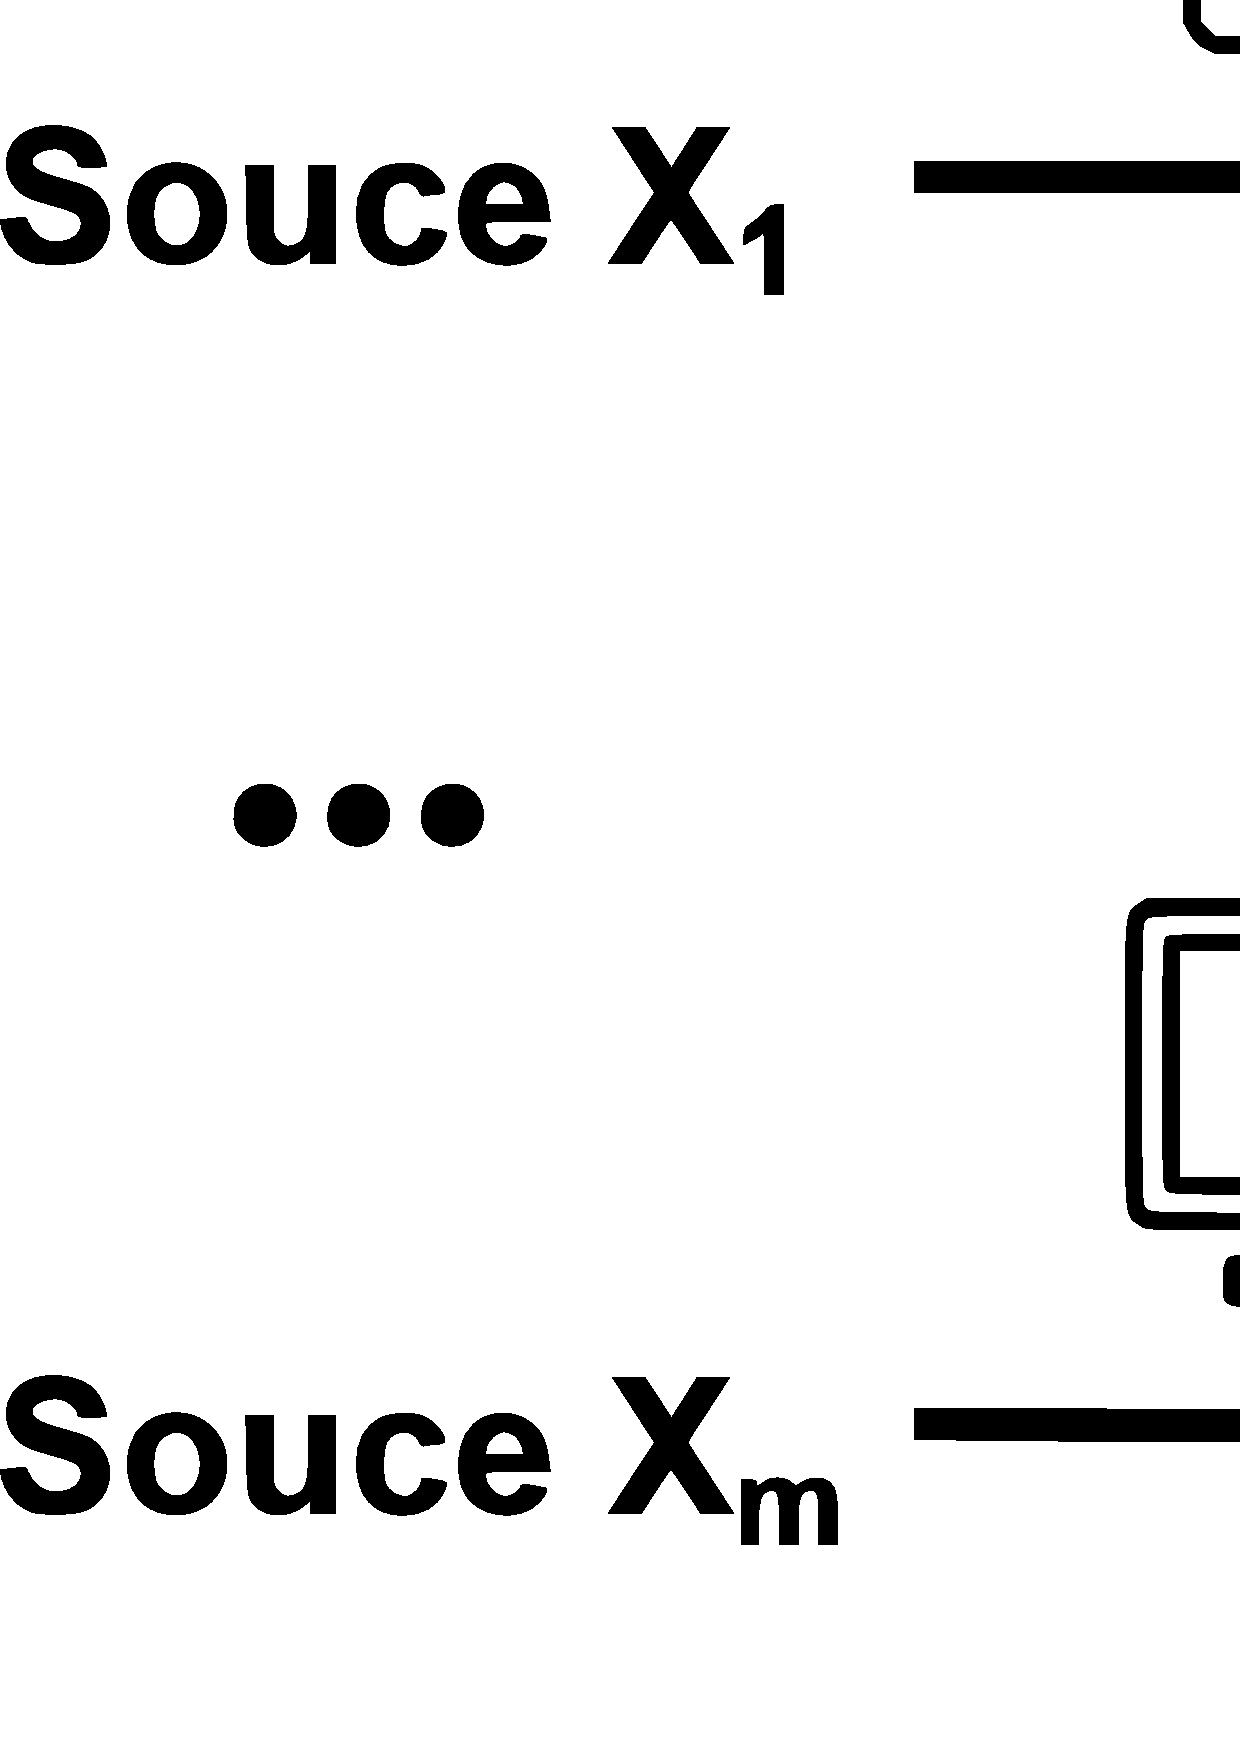
\includegraphics[width=1\linewidth]{DeepDSC.pdf}
\end{center}
   \caption{Illustration of Deep Distributed Source Coding.}
\label{fig_0}
\end{figure}

\begin{figure*}
\begin{center}
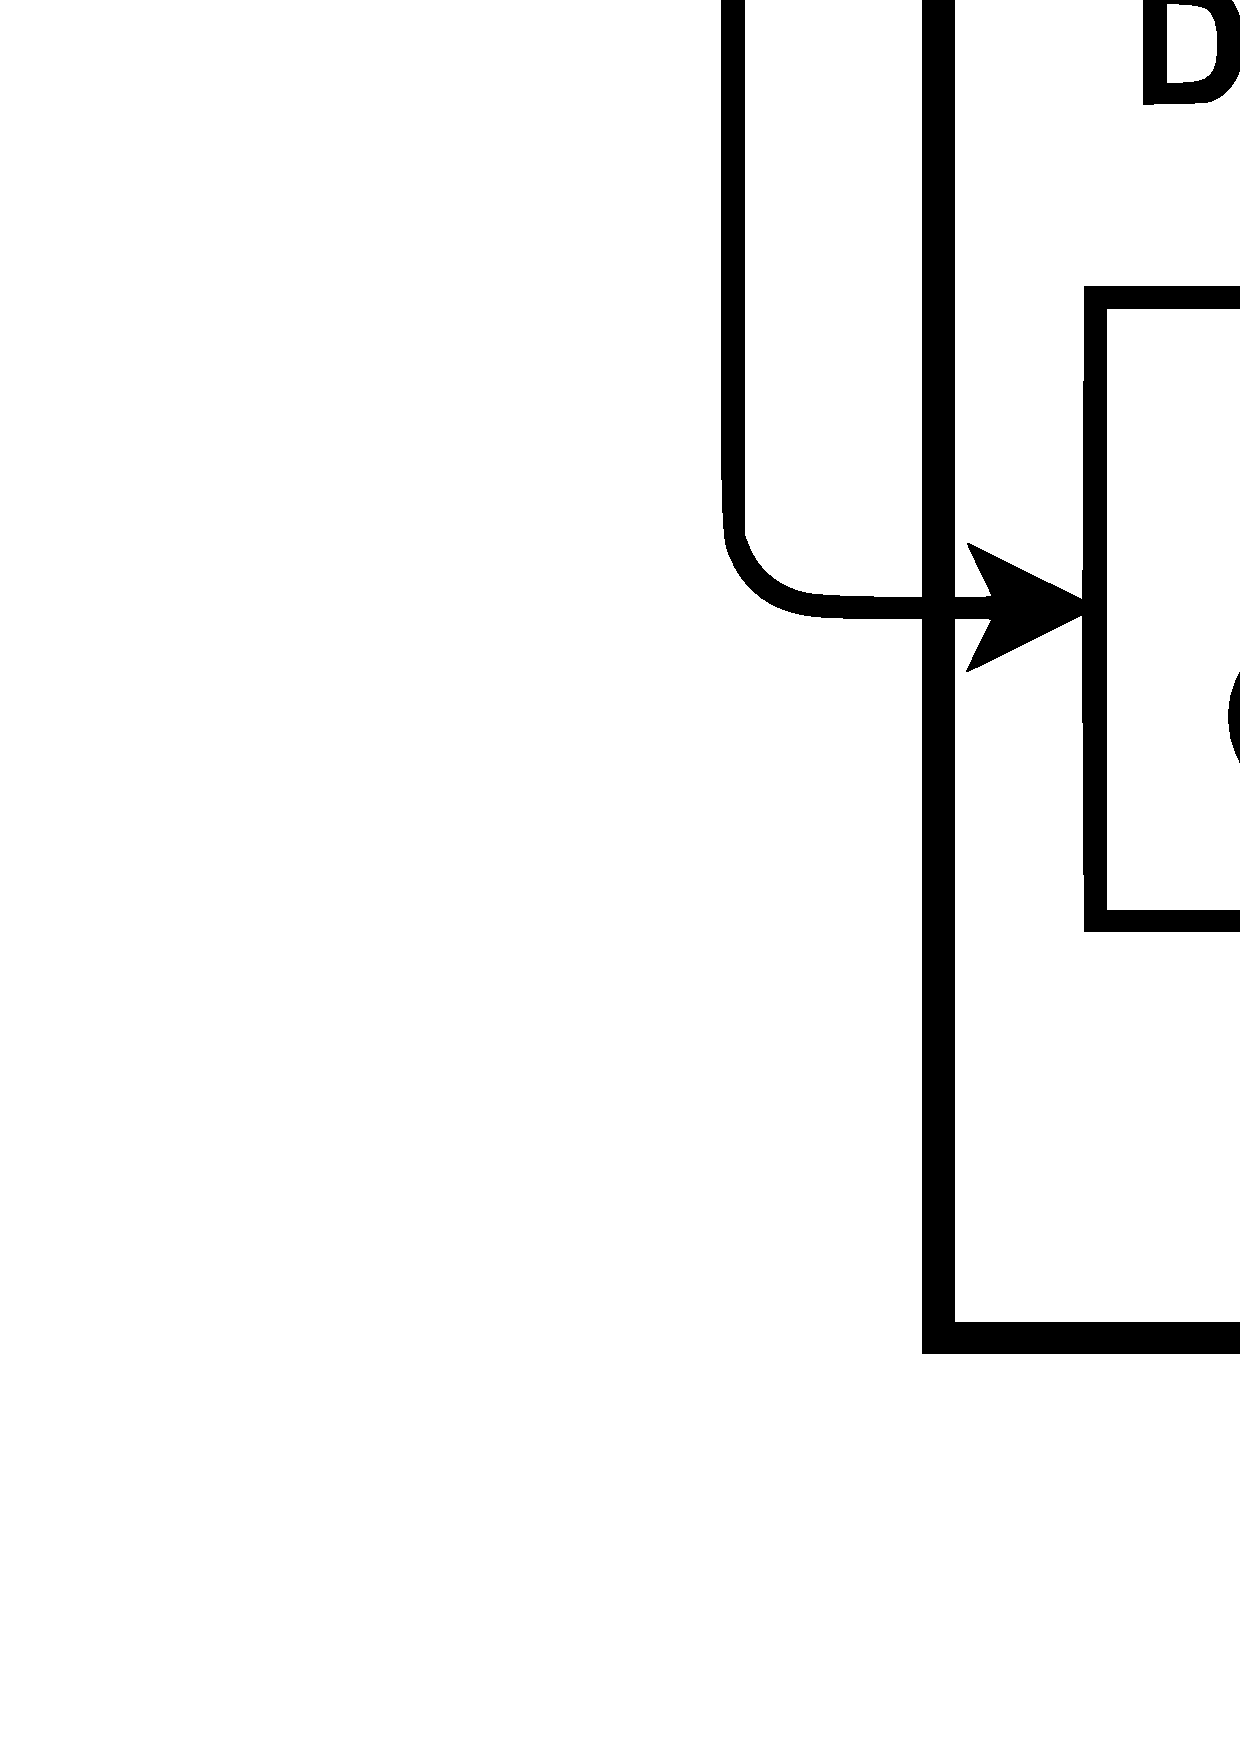
\includegraphics[width=0.8\linewidth]{DeepEncoderDecoder.pdf}
\end{center}
   \caption{Illustration of pixel-shuffled symmetric Encoder-Decoder architecture.}
\label{fig_1}
\end{figure*}
The advantages of our proposed architecture (illustrated in Fig.~\ref{fig_0} and \ref{fig_1}) are fourfold. 
First, the architecture is naturally scalable in the sense that codes can be decoded at more than one compression quality levels, and it allows efficient coding of correlated sources which are not physically co-located. This is especially attractive in video streaming applications \cite{guillemot2007distributed,gehrig2008distributed}. Second, unlike classical DSC which requires customized code design for different scenarios \cite{xiong2004distributed}, data-driven DSC framework can handle nontrivial distribution of image sources with arbitrary correlations. Third, the computation complexity of the encoder can be transferred to the decoder, a system of low complexity encoders can be used in a variety of application domains, such as multi-view video coding \cite{girod2005distributed}, sensor networks \cite{xiong2004distributed}, and under-water image processing where communication bandwidth and computational power are quite restricted \cite{stojanovic2009underwater,schettini2010underwater}. Fourth, the distributed framework can be more robust against heterogeneous noises or malfunctions of encoders, and such robustness can be crucial in, e.g., unreliable sensor networks \cite{girod2005distributed,ishwar2005rate,xiao2006distributed}.

The paper is outlined below. We review previous related work in Section 2 and describe our proposed method in details in Section 3. We describe our architecture for general image compression and its base modules in Section 3.1-3.4. Then we elaborate the Deep Distributed Source Coding framework in Section 3.5. Experimental results are shown in Section 4, followed by conclusions in Section 5.

%------------------------------------------------------------------------
\section{Related Work}
Though there has been a variety of research on lossy data compression in the past few decades, little attention has been paid to a systematic approach for general and practical distributed code design, especially in the presence of an arbitrary number of nontrivial data sources with arbitrary correlation %and possibly sources and correlation with memory. 
\cite{xiong2004distributed}. 
A main motivation of this work is to attempt to replace the practical hand-crafted code design with data-driven approaches. 
To our best knowledge, what we propose is the first data-driven DSC architecture. 
Unlike hand-crafted quantizers, our neural network-based quantizers show that the correlations among different data sources can be trained by the model parameters. We empirically show that the Slepian-Wolf limit can be achieved with our methodology. 

\subsection{Image compression with Deep Learning}
There exist a variety of classical codecs for lossy image compression. Although the JPEG standard \cite{wallace1992jpeg} was developed thirty years ago, it is still the most widely used image compression method. Several extensions to JPEG including JPEG2000 \cite{skodras2001jpeg}, WebP \cite{google2010webp} and BPG \cite{bellard2014bpg} have been developed. Most of these classical codecs rely on a quantization matrix applied to the coefficients of discrete cosine transform or wavelet transform.

The standard methods of compression with deep learning roughly fall into two categories. Non-recurrent autoencoders which rely on $\mathcal{L}_1$ penalty to sparsify the 8-bit integer codes, and recurrent models which introduce binary codes at each iteration. 
%Autoencoders are widely used as a general framework for neural network-based image compression. Bottleneck representations are quantized into 8-bit integers or binaries. 
The compression rate of non-recurrent models is not scalable and their performance heavily rely on the sparsity which entropy codec can take advantage of. 
Another challenge is to well define the derivative of quantizations of bottleneck representations. Ball\'e et al. \cite{balle2016end} replaced non-differentiable quantization step with a continuous relaxation by adding uniform noises. Toderici \cite{toderici2015variable}, on the other hand, used a stochastic form of binarization. 
The recurrent model~\cite{toderici2015variable,johnston2017improved}, on the other hand, has scalable compression rates. It generates more codes when the residual difference between the input and output of the model is compressed again.

\subsection{Distributed Source Coding}

\begin{figure}[t]
\begin{center}
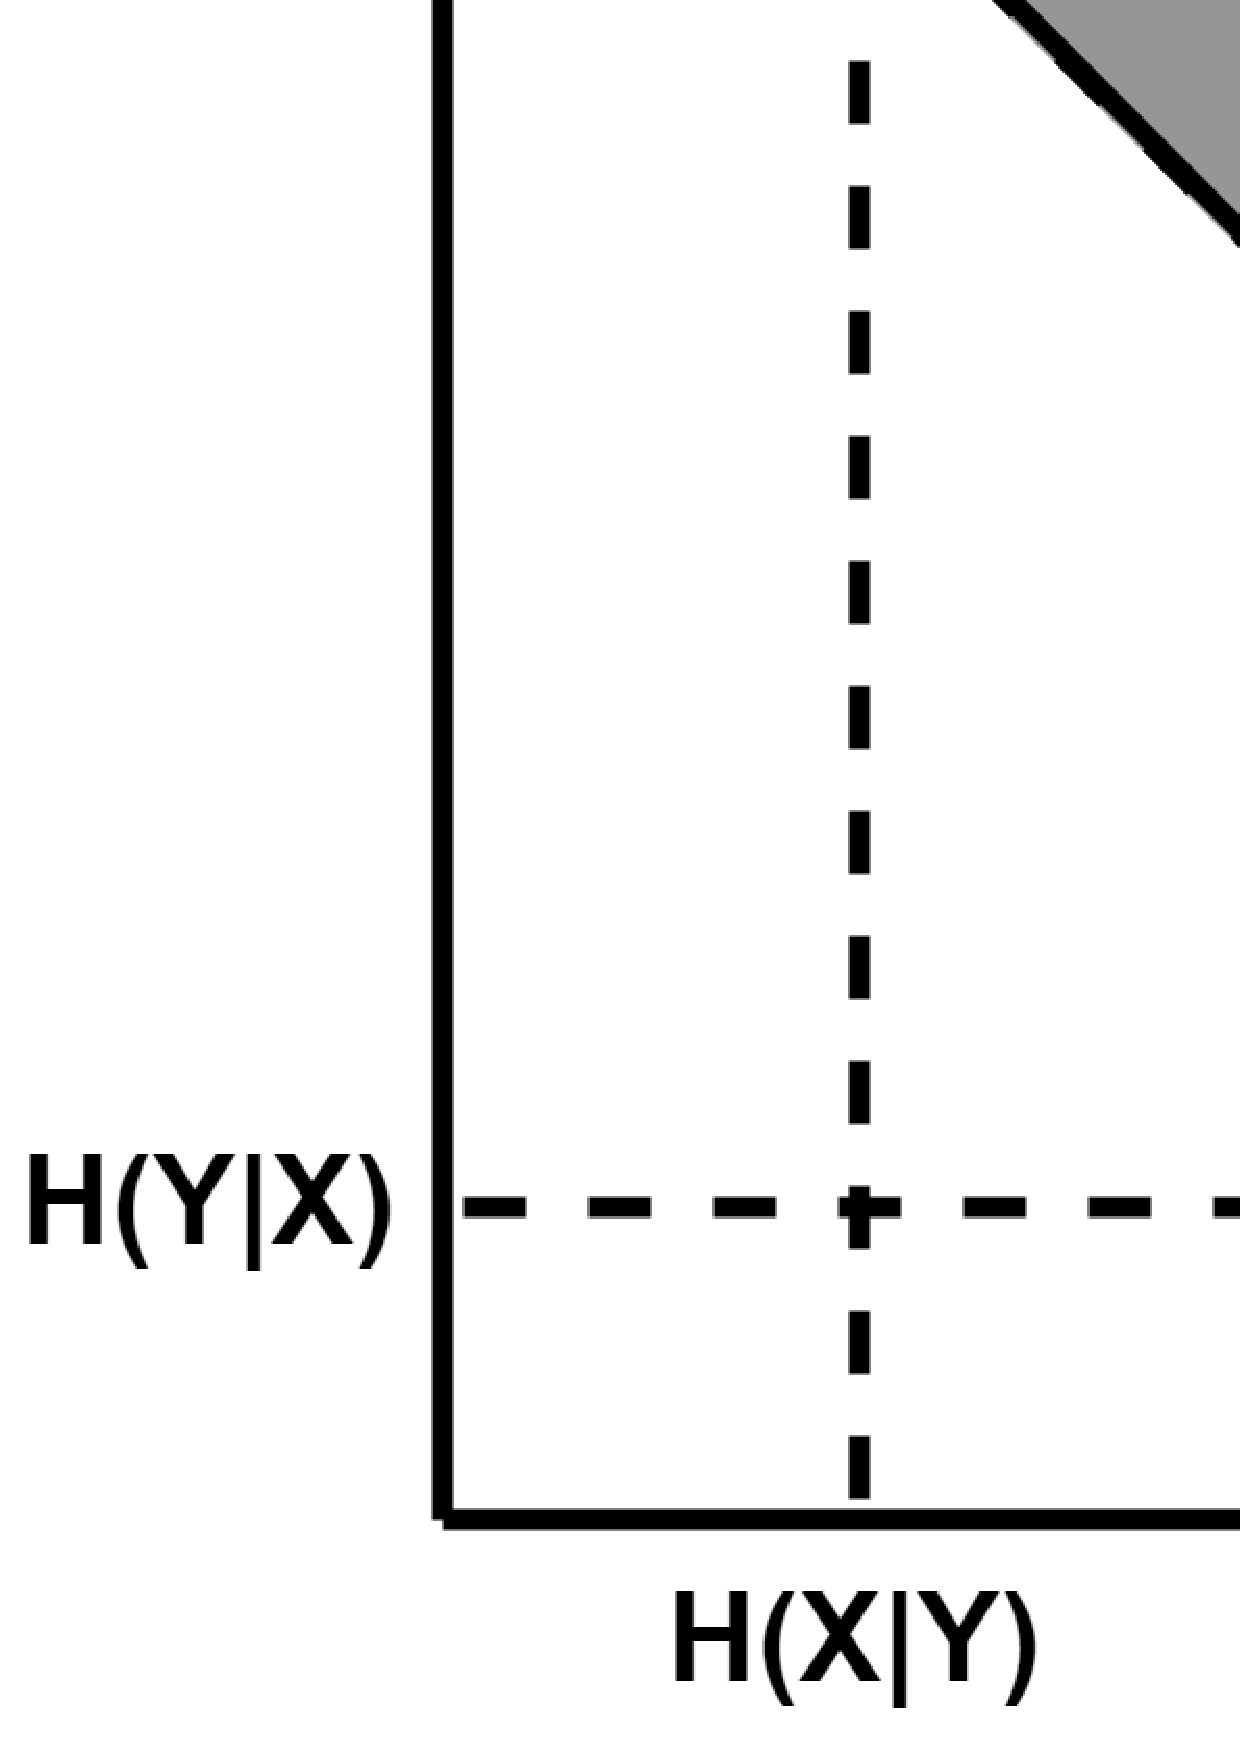
\includegraphics[width=0.8\linewidth]{SlepianWolf.pdf}
\end{center}
   \caption{The Slepian-Wolf achievable region for two sources $X$ and $Y$.}
\label{fig_2}
\end{figure}
Our methodology is deeply rooted in information-theoretic results on DSC which have been established since 1970s. The Slepian-Wolf \cite{slepian1973noiseless} Theorem shows that two correlated data sources encoded separately and decoded jointly can perform as well as joint encoding and decoding, and outperform separate encoding and separate decoding. The striking result indicates that as long as the codes are jointly decoded, there can be no loss in coding efficiency even the codes are separately encoded. Cover \cite{cover1975proof} generalizes the achievability of Slepian-Wolf coding to arbitrary number of correlated sources. Wyner-Ziv Coding \cite{wyner1976rate} gives a rate-distortion curve as an extension to lossy cases.

A classical illustration of Slepian-Wolf achievable region is shown in Fig.~\ref{fig_2}. We can achieve the performance of joint encoding and decoding of two data sources $X$ and $Y$ where the bit rate $R$ is equal to the joint entropy $H(X,Y)$ with separate encoding and joint decoding. Specifically, the achievable region proved by the Slepian-Wolf Theorem is given by $R_X\geq H(X|Y),R_Y\geq H(Y|X),$ and $R_X+R_Y\geq H(X,Y)$ as shown in the shaded area of Fig.~\ref{fig_2}. Here $R_{\cdot},H(\cdot)$ denote the bit rates and (conditional) entropies in classical Shannon theory. In practice, although some works are proposed to approach the mid-point $C$ \cite{schonberg2004distributed}, the most widely used scheme is source coding with side information (syndrome bits) at the decoder \cite{pradhan2003distributed}. This code design takes advantage of the corner points $A$ and $B$ which correspond to $R(X,Y) = R(Y)+R(X|Y)$ and $R(X,Y) = R(X)+R(Y|X)$ respectively. As an example, two 8-bit grayscale images $X$ and $Y$ have pixel values at the same location with (nonlinear) correlation implicitly determined by $x \in \{y-4, y-3, y-2, y-1, y, y+1, y+2, y+3\}$. Instead of sending 16 bits, we can send bits with $R=H(Y)+H(X|Y)$. We can take modulo of $x-y$ with respect to $8$ which only requires a 3-bit codebook $\tilde{x} \in \{4, 5, 6, 7, 0, 1, 2, 3\}$. Specifically, for $x=124$ and $y=128$, we transmit $\tilde{x}=(x-y) \mod 8$ which is 4 and $y=128$. The joint decoder will decode $x$ based on $y$ as $x = y-4 = 124$.

Some researchers have also shown the applicability of DSC on still images \cite{dikici2005distributed}. In practical applications, low complexity video encoding benefits from the DSC framework which can transfer the complexity of encoder to decoder \cite{puri2002prism,aaron2002wyner}. Scalable Video Coding can also be incorporated with DSC \cite{xu2006layered}. These proposed methods indicate the feasibility of DSC in our problem setting.

%-------------------------------------------------------------------------
\section{Methods}
In this section, we first describe the symmetric Encoder-Decoder architecture used in our research work. We will elaborate the base modules including Convolutional Long short-term memory (ConvLSTM), Pixel (Un)Shuffle, and Binarizer used in our model. We will then describe how this Deep Learning architecture is used in Distributed Source Coding framework.

\subsection{Network Architecture}
Our compression network consists of an encoder, a binarizer, and a decoder. The activation function following each Convolutional Neural Network (CNN) module is $\tanh$. For the first iteration of our model, the input images are initially encoded and transformed into $(-1,1)$ by $\tanh$ activation function. Binary codes are quantized from transformed bottleneck representations. The decoder then reconstructs images based on the received binary codes. Finally, we compute the residual difference between the original input images and the reconstructed output images. At the next iteration, the residual difference is feedback as the new input for our model. This procedure is repeated multiple iterations to gain more codes for better reconstruction performance. Therefore, the reconstructed images at each iteration are the sum of output reconstructions from previous and current iterations.

Consider dataset $X = \{x\}^{N}$ consisting of $N$ i.i.d. samples of some continuous or discrete variables $x$. The data generating process is unknown. Autoencoders for compression and reconstruction can be formulated in the following way. Data can be compressed with a neural network-based encoder $f(x;\theta)$ into quantized codes $\tilde{z}$ and reconstructed with a decoder $g(\tilde{z};\phi)$. We can binarize bottleneck representations $z$ and control the compression quality by varying its channel sizes. The loss function $\mathcal{L}(x,\tilde{x})$ is minimized with respect to the model parameters $\theta$ and $\phi$.
\begin{align}
z &= f(x;\theta),\\
\tilde{z} &= \text{Binarize}(z),\\
\tilde{x} &= g(\tilde{z};\phi),\\
\text{Minimize } \mathcal{L}&(x,\tilde{x})
\end{align}
Deep recurrent autoencoder gradually increases compression quality by creating a correlated residual sequence from the difference between the input and output of our model. The advantage of recurrent model is that we can train one model with scalable compression quality. Classical autoencoders, on the contrary, have to train multiple networks with different penalty coefficients or channel sizes for different compression qualities. Suppose $T$ iterations are used, we can formulate the recurrent autoencoder in the following way.
\begin{align}
z_t &= f(x_t;\theta),\\
\tilde{z}_t &= \text{Binarize}(z_t),\\
\tilde{x}_t &= g(\tilde{z}_t;\phi),\\
x_{t+1} &= x_t-\tilde{x}_t\text{, }\tilde{x}_1=0,\\
\text{Minimize } \frac{1}{T}&\sum_{t=1}^{T}\mathcal{L}(x_1,\sum_{i=1}^{t}\tilde{x}_i).
\end{align}
In the recurrent autoencoder, the compression quality is controlled by several factors including the scale factor of Pixel (Un)Shuffle module $r$, the depth of model $D$, the channel size of bottleneck representations $C$, and the number of iterations $T$. The height and width of bottleneck representations are determined by $T$ and $D$. As we have $N$ batch images with shape $H,W$, the size of codes after $T$ iterations is $(N,T,C,H/(r^D),W/(r^D))$. For example, with $r=2$, $D=3$, and $C=2^D$, one $32 \times 32$ RGB image will generate $(1,1,8,4,4)$ binary codes for a single iteration. Thus, we will add up $\frac{8
\times4\times4}{32\times32} = 0.125$ Bit Per Pixel (BPP) for this iteration. Although we configure these hyper-parameters, we believe it is possible to train these configurations in future works.

\subsection{Convolutional Long short-term memory}
As proposed by \cite{xingjian2015convolutional}, simply replacing the Fully Connected (FC) layer in LSTM with convolutional layer, ConvLSTM is able to capture spatial structure in the temporal sequence. We do not add any bias term to our modules because the output of each layer is saturated by $\tanh$. The key equations are shown below.
\begin{align}
i_t &= \sigma(W_{xi}*x_t + W_{hi}*h_{t-1}) ,\\
f_t &= \sigma(W_{xf}*x_t + W_{hf}*h_{t-1}) ,\\
c_t &= f_tc_{t-1}+i_t\tanh(W_{xc}*x_t + W_{hc}*h_{t-1}), \\
o_t &= \sigma(W_{xo}*x_t + W_{ho}*h_{t-1}) ,\\
h_t &= o_t\tanh(c_t).
\end{align}
The first and last layers of the encoder and decoder are feed-forward Convolutional Neural Network with $\tanh$ activations. The recurrent layers are all ConvLSTM networks. We do not replace CNN layer with ConvLSTM because the size of the feature maps of hidden state at shallow layers cost a mass amount of memory. From our various experimental studies, the performance does not degrade significantly either because no convolutional layers are in between ConvLSTM layers.

\subsection{Pixel (Un)Shuffle}
We resize feature maps with Pixel (Un)Shuffle modules. Pixel Shuffle module is originally proposed by \cite{shi2016real} to tackle image and video super-resolution problem. Compared to bilinear interpolation and tranposed convolutional layers, Pixel Shuffle module is much more computationally efficient, because it is non-parametric and only requires tensor reshaping and dimension permutation. We note that although this method is widely used for upscaling, it is actually invertible and we propose to use its inversion for downscaling. Thus, the encoder and decoder can be constructed symmetrically. Our experimental results show that symmetric Encoder-Decoder architecture actually produces much better results with less number of parameters, compared to the asymmetric architecture as proposed in \cite{toderici2017full}. We describe these two modules with the following pseudocodes \ref{alg_0} and \ref{alg_1}.

\begin{algorithm}
\caption{Pixel UnShuffle}
\begin{algorithmic}
\label{alg_0}
\REQUIRE $X\sim(N,C,H,W)$, $r_H,r_W$
\ENSURE $r_H,r_W$ are integers, divides $H,W$
\STATE Reshape $X\sim(N,C,H/r_H,r_H,W/r_W,r_W)$
\STATE Permute $X\sim(N,C,r_H,r_W,H/r_H,W/r_W)$
\STATE Reshape $X\sim(N,C\times r_H\times r_W,H/r_H,W/r_W)$
\end{algorithmic}
\end{algorithm}

\begin{algorithm}
\caption{Pixel Shuffle}
\begin{algorithmic}
\label{alg_1}
\REQUIRE $X\sim(N,C,H,W)$, $r_H,r_W$
\ENSURE $r_H,r_W$ are integers, $r_H\times r_W$ divides $C$
\STATE Reshape $X\sim(N,C/(r_H \times r_W),r_H,r_W,H,W)$
\STATE Permute $X\sim(N,C/(r_H \times r_W),H,r_H,W,r_W)$
\STATE Reshape $X\sim(N,C/(r_H \times r_W),H \times r_H,W \times r_W)$
\end{algorithmic}
\end{algorithm}

\subsection{Binarizer}
The derivative of quantization function is only defined at the rounded integer itself. Therefore, we have to replace its derivative in the backward pass of backpropagation with a form of smooth approximation \cite{rumelhart1988learning}. Thanks to a thorough discussion of different alternative approaches by \cite{theis2017lossy}, we choose to use identity function to replace its derivatives that cannot be well defined as shown in \ref{eq_15}. During training, we use a stochastic form of binarization proposed by \cite{toderici2017full}. For bottleneck representations $z \in (-1,1)$, the details of binarizer $\tilde{z}=\text{Binarize}(z)$ are described as follows, where $W_{\cdot}$ denote the standard parameter matrices between two network layers.
\begin{align}
\intertext{\textbf{Train}}
\tilde{z}=\text{Binarize}(z) &= 
    \begin{cases}
      1, &  \text{with probability } (z+1)/2\\
      -1, & \text{otherwise}
      \end{cases} \nonumber \\
\frac{d}{dz}\tilde{z} &:= \frac{d}{dz}\mathbb{E} (\tilde{z}) =  \frac{d}{dz}\mathbb{E} (z) = 1\label{eq_15}
\intertext{\textbf{Test}}
\text{Binarize}(z) &= 
    \begin{cases}
      1, & \text{if } z\geq0 \\
      -1, & \text{otherwise}
      \end{cases}
\end{align}

\subsection{Deep Distributed Source Coding Framework}
Fig.~\ref{fig_0} and \ref{fig_1} illustrates our Deep DSC coding framework. Similar to classical DSC framework, each data source is encoded separately and decoded jointly. Traditionally, researchers have to design different kind of codes for specific scenarios \cite{schonberg2004distributed}. We propose to use data-driven approach to handle complex scenarios where the distribution of data sources are unknown and their correlations can be arbitrary. Our proposal may also shed new light on sophisticated application scenarios such as videos where data sources and correlations are time dependent.

In our neural network-based DSC, %the whole encoding and decoding procedure are trained jointly. 
$M$ distributed encoders encode corresponding data sources $x^m$ that can be arbitrarily correlated. Each neural network-based encoder $f(x^m;\theta^m)$ has their own model parameters $\theta^m$. After binarizing bottleneck representations $z^m$, code sources $\tilde{z}^m$ are transmitted and concatenated batch-wisely. A single decoder $g(\tilde{z}^m;\phi)$ reconstructs images $\tilde{x}^m$ from all sources with the same model parameters $\phi$. 
In particular, the parameters of the following model are optimized with backward propagation \cite{rumelhart1988learning}. 
\begin{align}
z_t^m &= f(x_t^m;\theta^m),\\
\tilde{z}_t^m &= \text{Binarize}(z_t^m),\\
\tilde{x}_t^{m} &= g(\tilde{z}_t^{m};\bm{\phi}),\\
x_{t+1}^{m} &= x_t^{m}-\tilde{x}_t^{m}\text{, }\tilde{x}_1^{m}=0,
\end{align}
\begin{align}
\text{Minimize } \frac{1}{MT}&\sum_{t=1}^{T}\sum_{m=1}^{M}\mathcal{L}(x_1^m,\sum_{i=1}^{t}\tilde{x}_i^m).
\end{align}
Our result shows that the resulting distributed model can perform as well as encoding all data by one single encoder. However, if we encode and decode each data source separately, the performance becomes significantly worse. Moreover, correlations among data sources cannot be learned with separate parameters of decoders, i.e. with 
$\tilde{x}_t^{m} = g(\tilde{z}_t^{m};\bm{\phi^m})$.
%------------------------------------------------------------------------
\section{Experiments}
We use MNIST dataset \cite{lecun1998gradient} consisting of 60,000 training and 10,000 testing grayscale handwritten digit images. The digits have been resized from $28 \times 28$ to $32 \times 32$. The Adam optimizer \cite{kingma2014adam} is used with $\epsilon = 1e-8$, $\beta_1 = 0.9$ and $\beta_2 = 0.999$. We train model with $\mathcal{L}_1$ loss, batch size $N=100$ and learning rate $0.001$ for a total of 200 epochs. We start to decay learning rate by half at the 70th epoch and at every 20 epochs thereafter.

As described in section 3.1, we set the scaling factor for Pixel (Un)Shuffle module to be $r=2$, depth of model $D=3$, and code channel size $C=2^D$. For $T=16$, one minibatch of grayscale images with shape $(100,1,32,32)$ will be encoded to be a $(100,16,8,4,4)$ binary tensor. We evaluate all models with the metric Peak Signal to Noise Ratio (PSNR) against the Bit Per Pixel (BPP).

\begin{figure}[t]
\begin{center}
\includegraphics[width=0.8\linewidth]{codec.pdf}
\end{center}
	\vspace{-0.2cm}
   \caption{Our symmetric pixel-shuffled Encoder-Decoder outperforms classical codecs and baseline neural network-based codecs.}
   \vspace{-0.2cm}
\label{fig_3}
\end{figure}

We compare our model to the baseline model \cite{toderici2017full} and classical codecs like JPEG~\cite{wallace1992jpeg}, JPEG2000~\cite{skodras2001jpeg} and BPG~\cite{bellard2014bpg}. To directly compare the performance of network architecture, we ignore some techniques introduced by \cite{toderici2017full} and \cite{johnston2017improved} such as progressive entropy coding and hidden-state priming. Instead of bilinear interpolation or convolutional layers used in previous works\cite{toderici2017full,theis2017lossy,johnston2017improved}, our network architecture uses Pixel Shuffle in the Encoder. As a result, our network architecture has a symmetric Encoder-Decoder structure and also few number of parameters. Fig.~\ref{fig_3} shows that our symmetric pixel-shuffled Encoder-Decoder architecture outperforms classical codecs and baseline neural network-based codecs.

We run experiments with $(2,4,8,10)$ number of distributed sources. Each encoder encodes data from each data source without communicating with other encoders. The decoder jointly decodes the codes gathered from each distributed encoder. First, we compare our result, labeled as \textit{Distributed}, to the case where all data are trained with one encoder and one decoder jointly, labeled as \textit{Joint}. The `Joint' curve is approximated as the theoretical upper bound of performance. %theoretical upper bound $H(X,Y)$. 
Second, we compare our result to the case where each data source is trained with a separate pair of encoder and decoder, labeled as \textit{Separate}. We test each distributed encoder separately with all test data. The solid curves are the average performance across all encoders. At each iteration, the confidence band is determined by the best and worst performance of all encoders. 

Our experimental studies in the following sections consist of three aspects. We first experiment data sources with different correlations. We then show the performance of low complexity encoders which are trained with less number of iterations. Finally, we show the robustness of our distributed framework in the absence of a number of distributed sources.

\begin{figure*}
\begin{center}
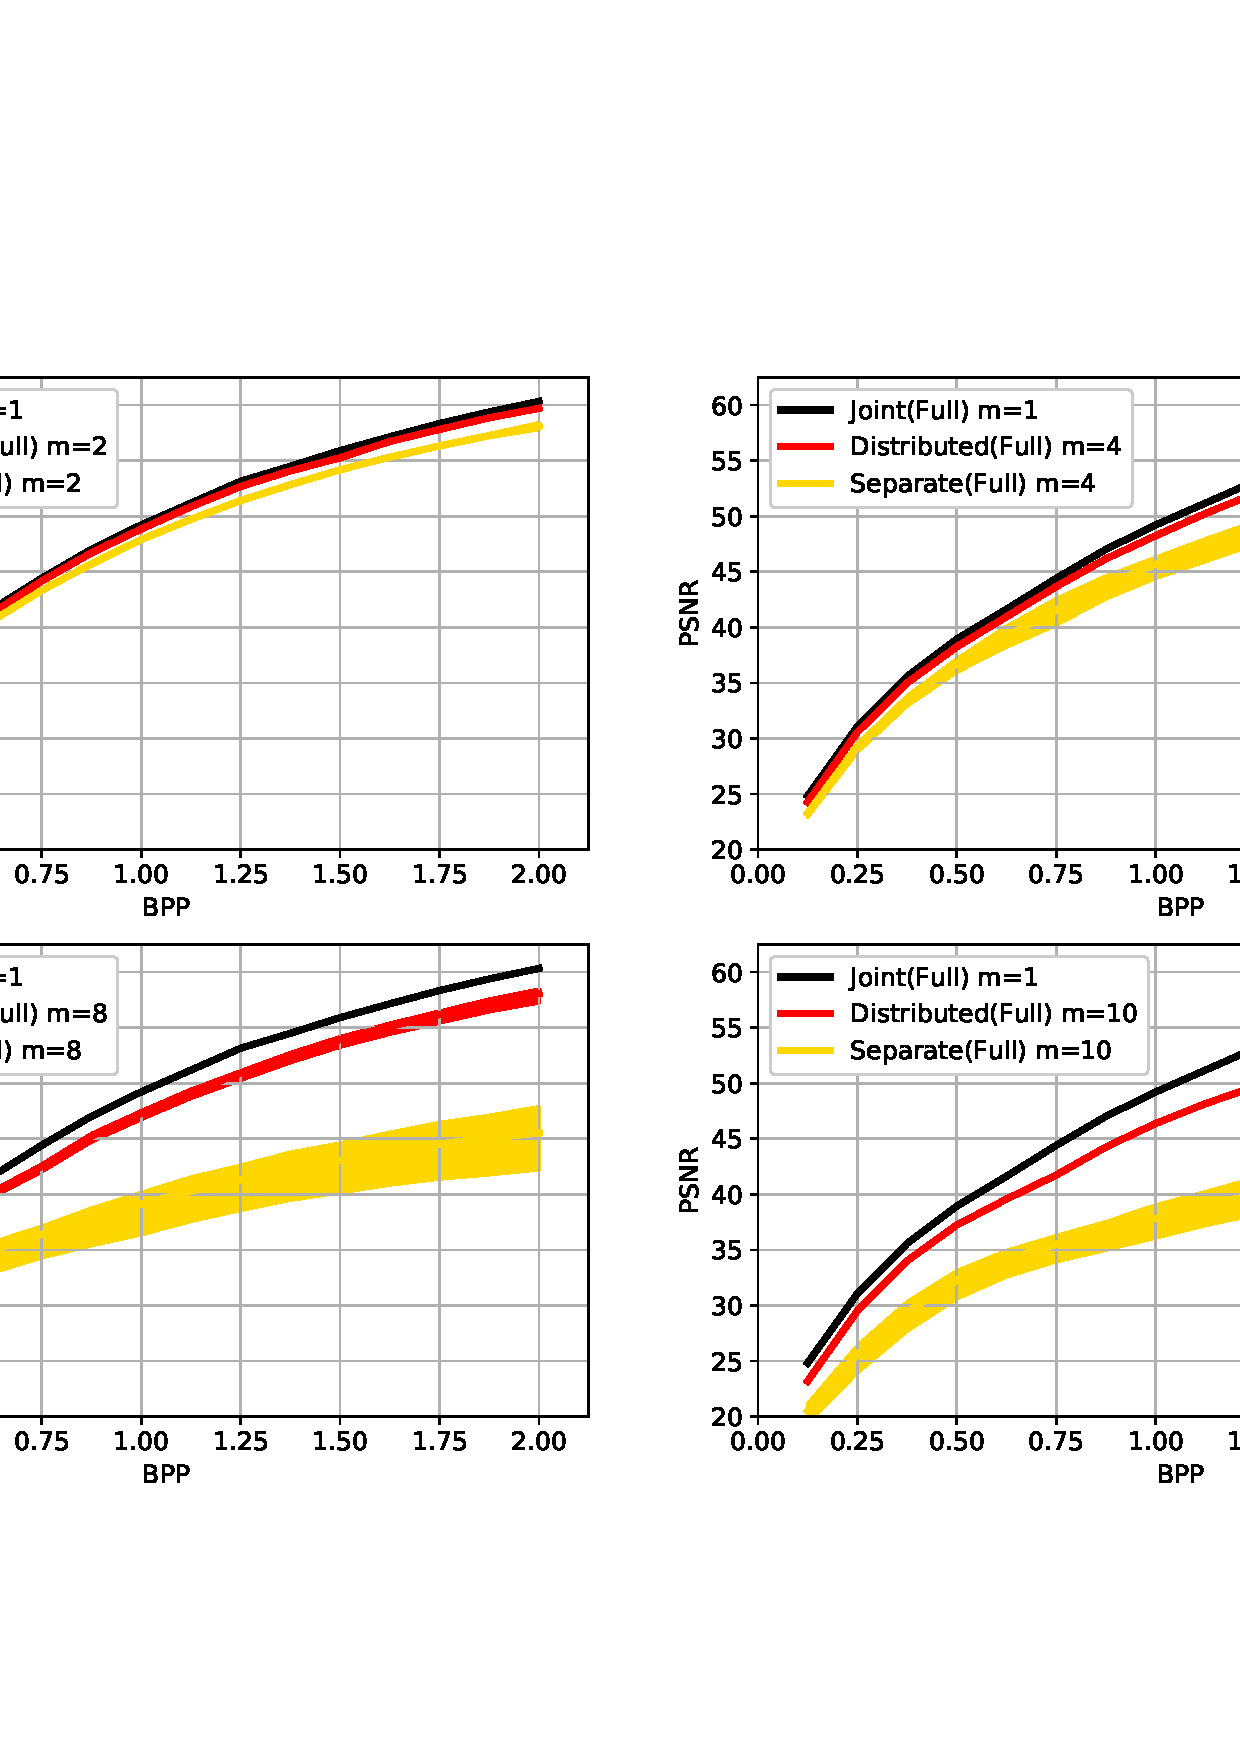
\includegraphics[width=0.8\linewidth]{full_subset_band.png}
\end{center}
	\vspace{-0.2cm}
   \caption{Rate-distortion curves for data sources distributed by random subsets with $T=16$ for all sources.}
   \vspace{-0.2cm}
\label{fig_4}
\end{figure*}

\begin{figure*}
\begin{center}
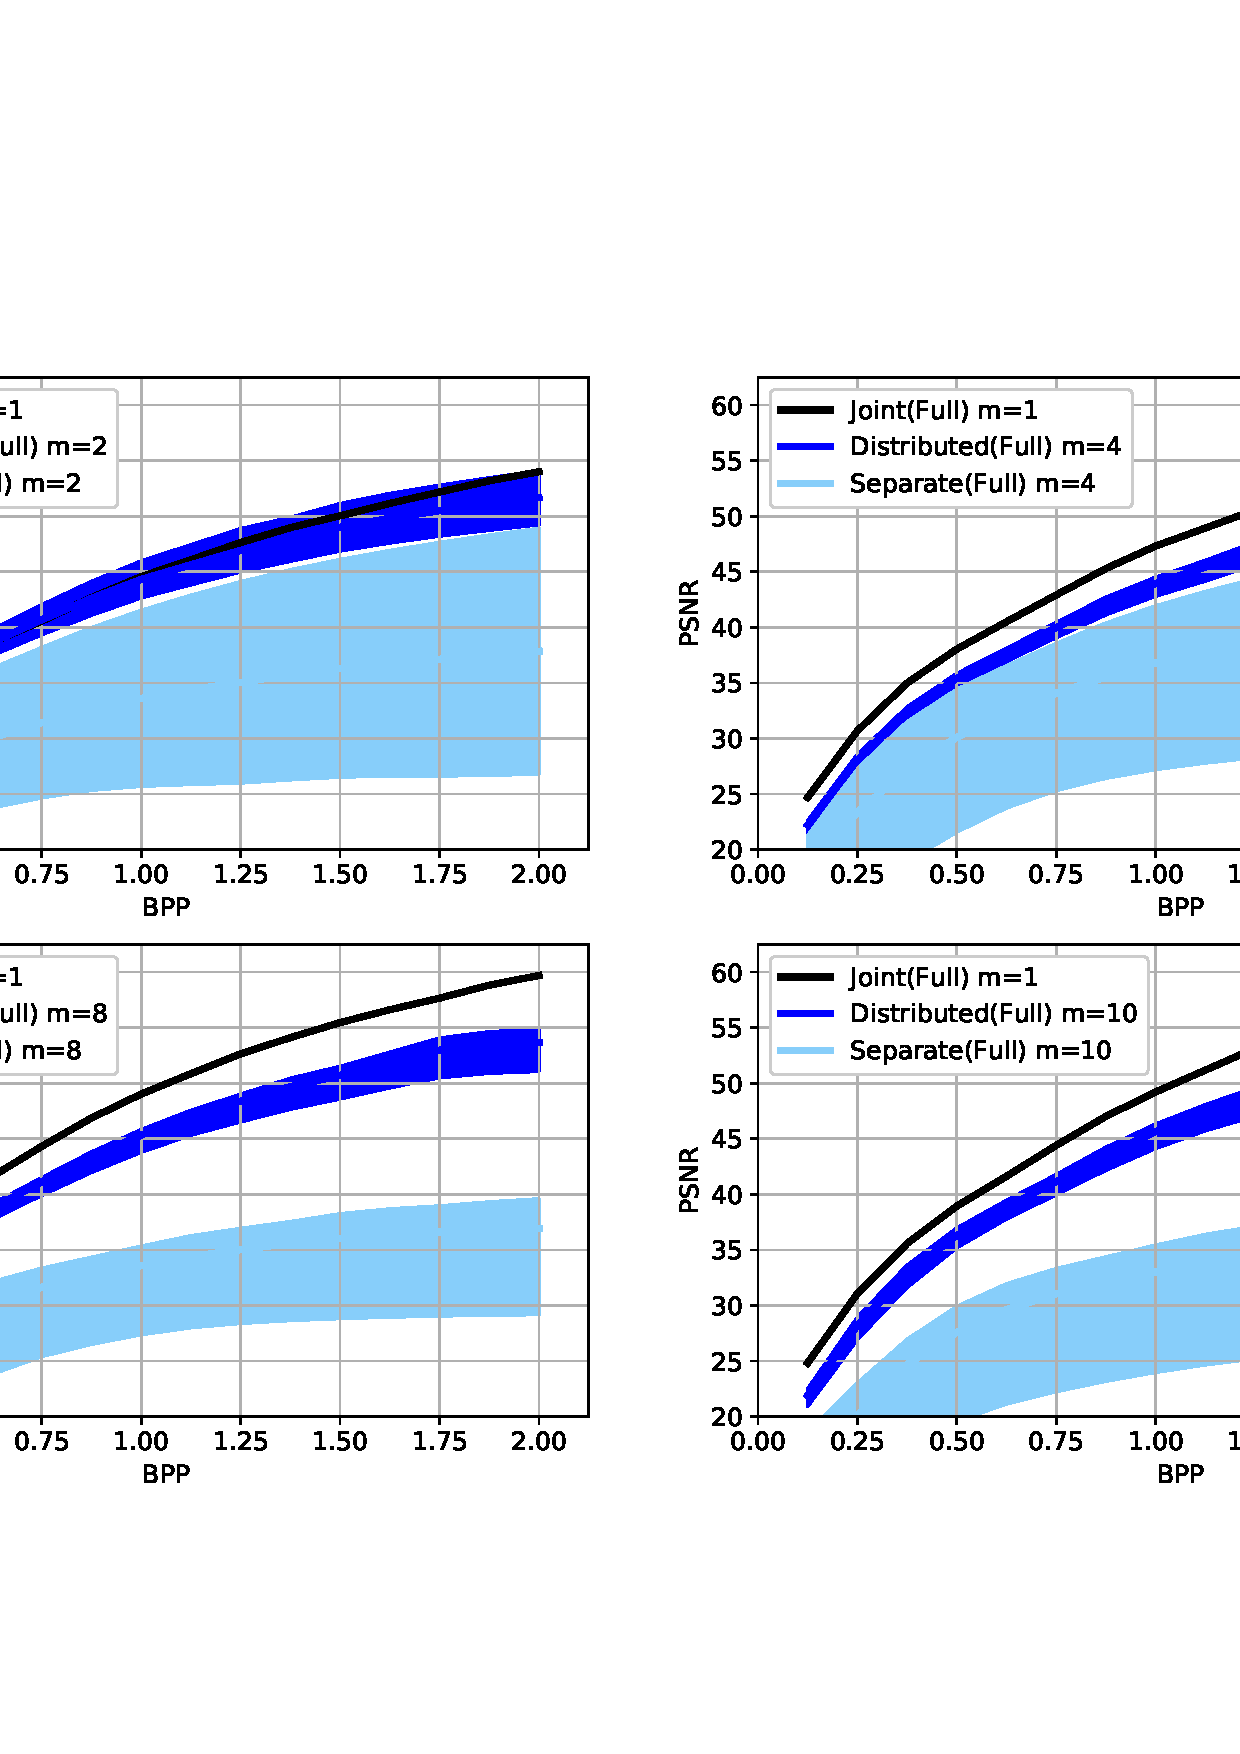
\includegraphics[width=0.8\linewidth]{full_class_band.png}
\end{center}
	\vspace{-0.2cm}
   \caption{Rate-distortion curves for data sources distributed by class labels with $T=16$ for all sources.}
   \vspace{-0.2cm}
\label{fig_5}
\end{figure*}

\begin{figure*}
\begin{center}
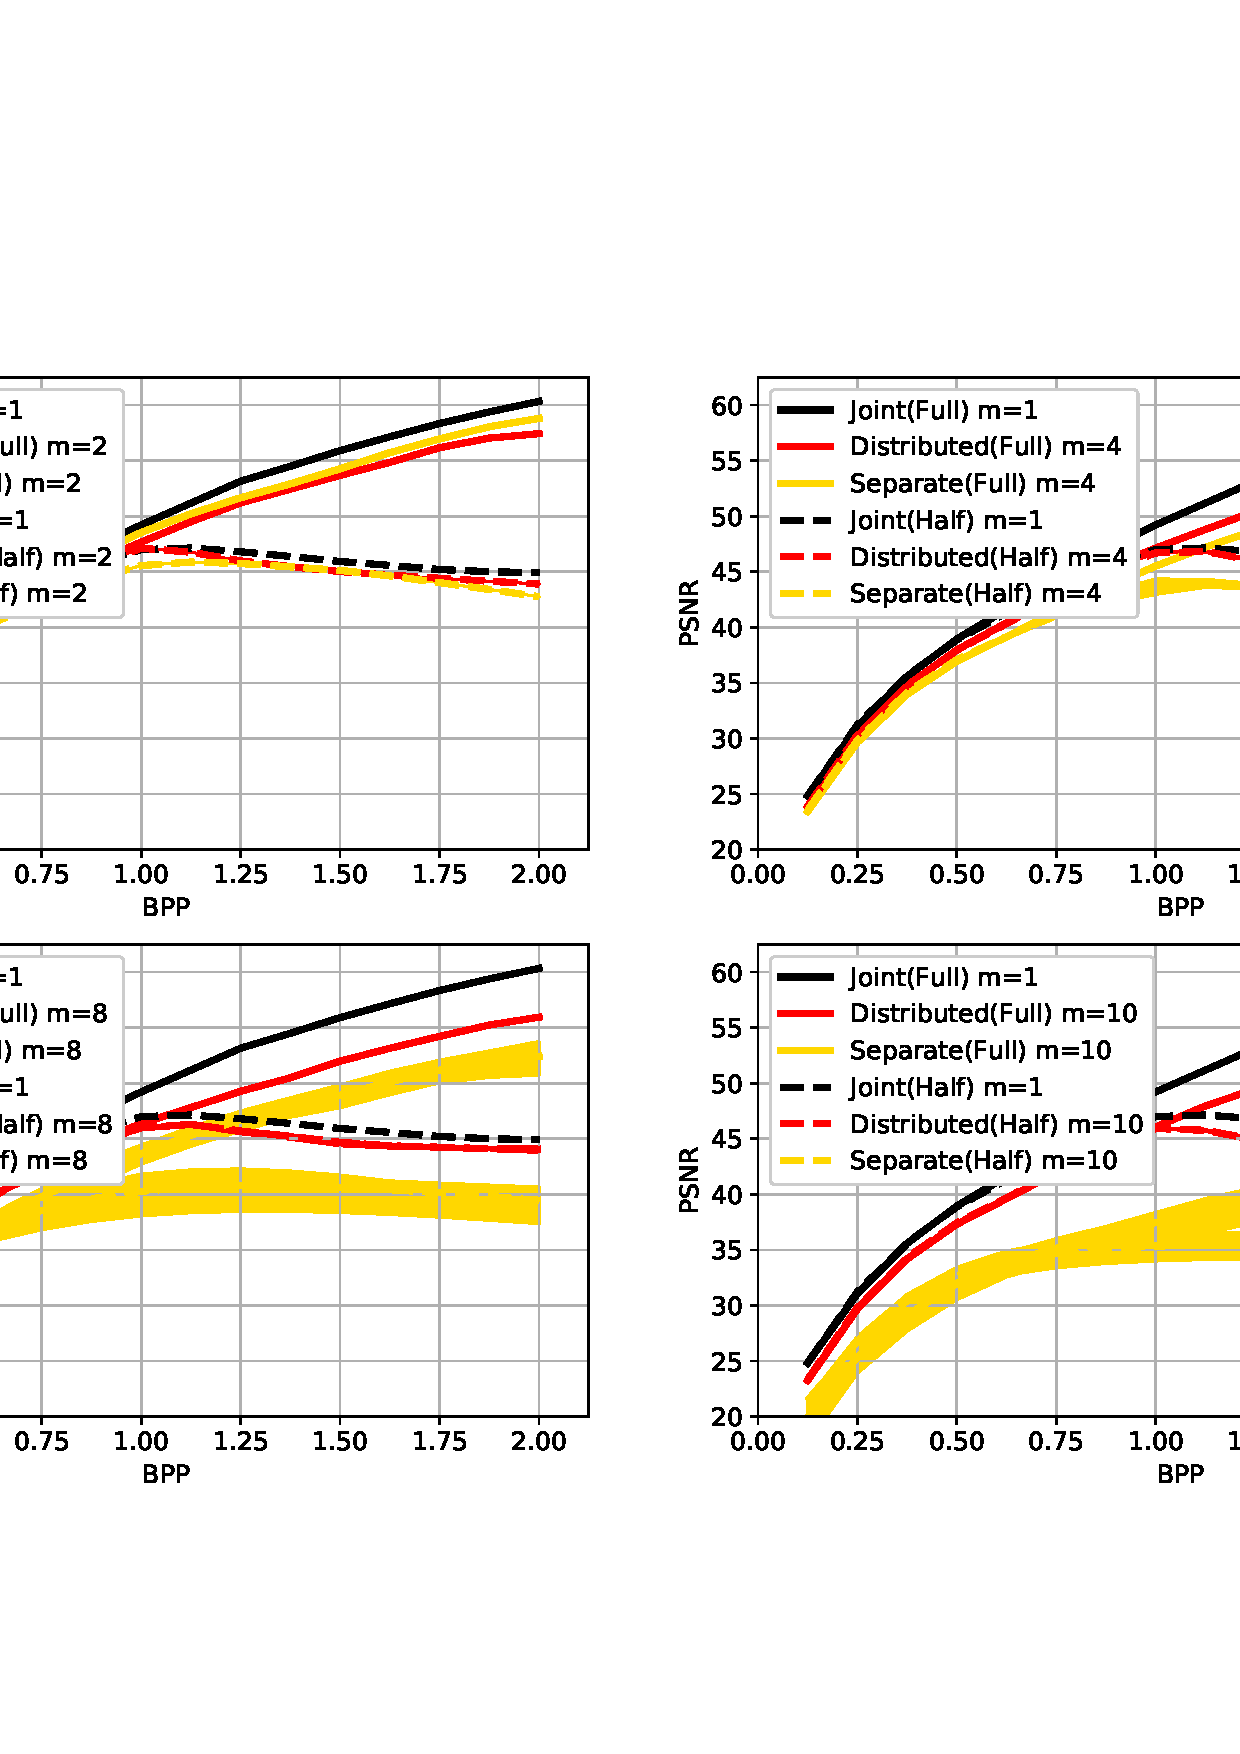
\includegraphics[width=0.8\linewidth]{half_subset_band.png}
\end{center}
	\vspace{-0.2cm}
   \caption{Rate-distortion curves for data sources distributed by random subsets with $T=16$ for the first half of sources and $T=8$ for the second half of sources.}
   \vspace{-0.2cm}
\label{fig_6}
\end{figure*}

\begin{figure*}
\begin{center}
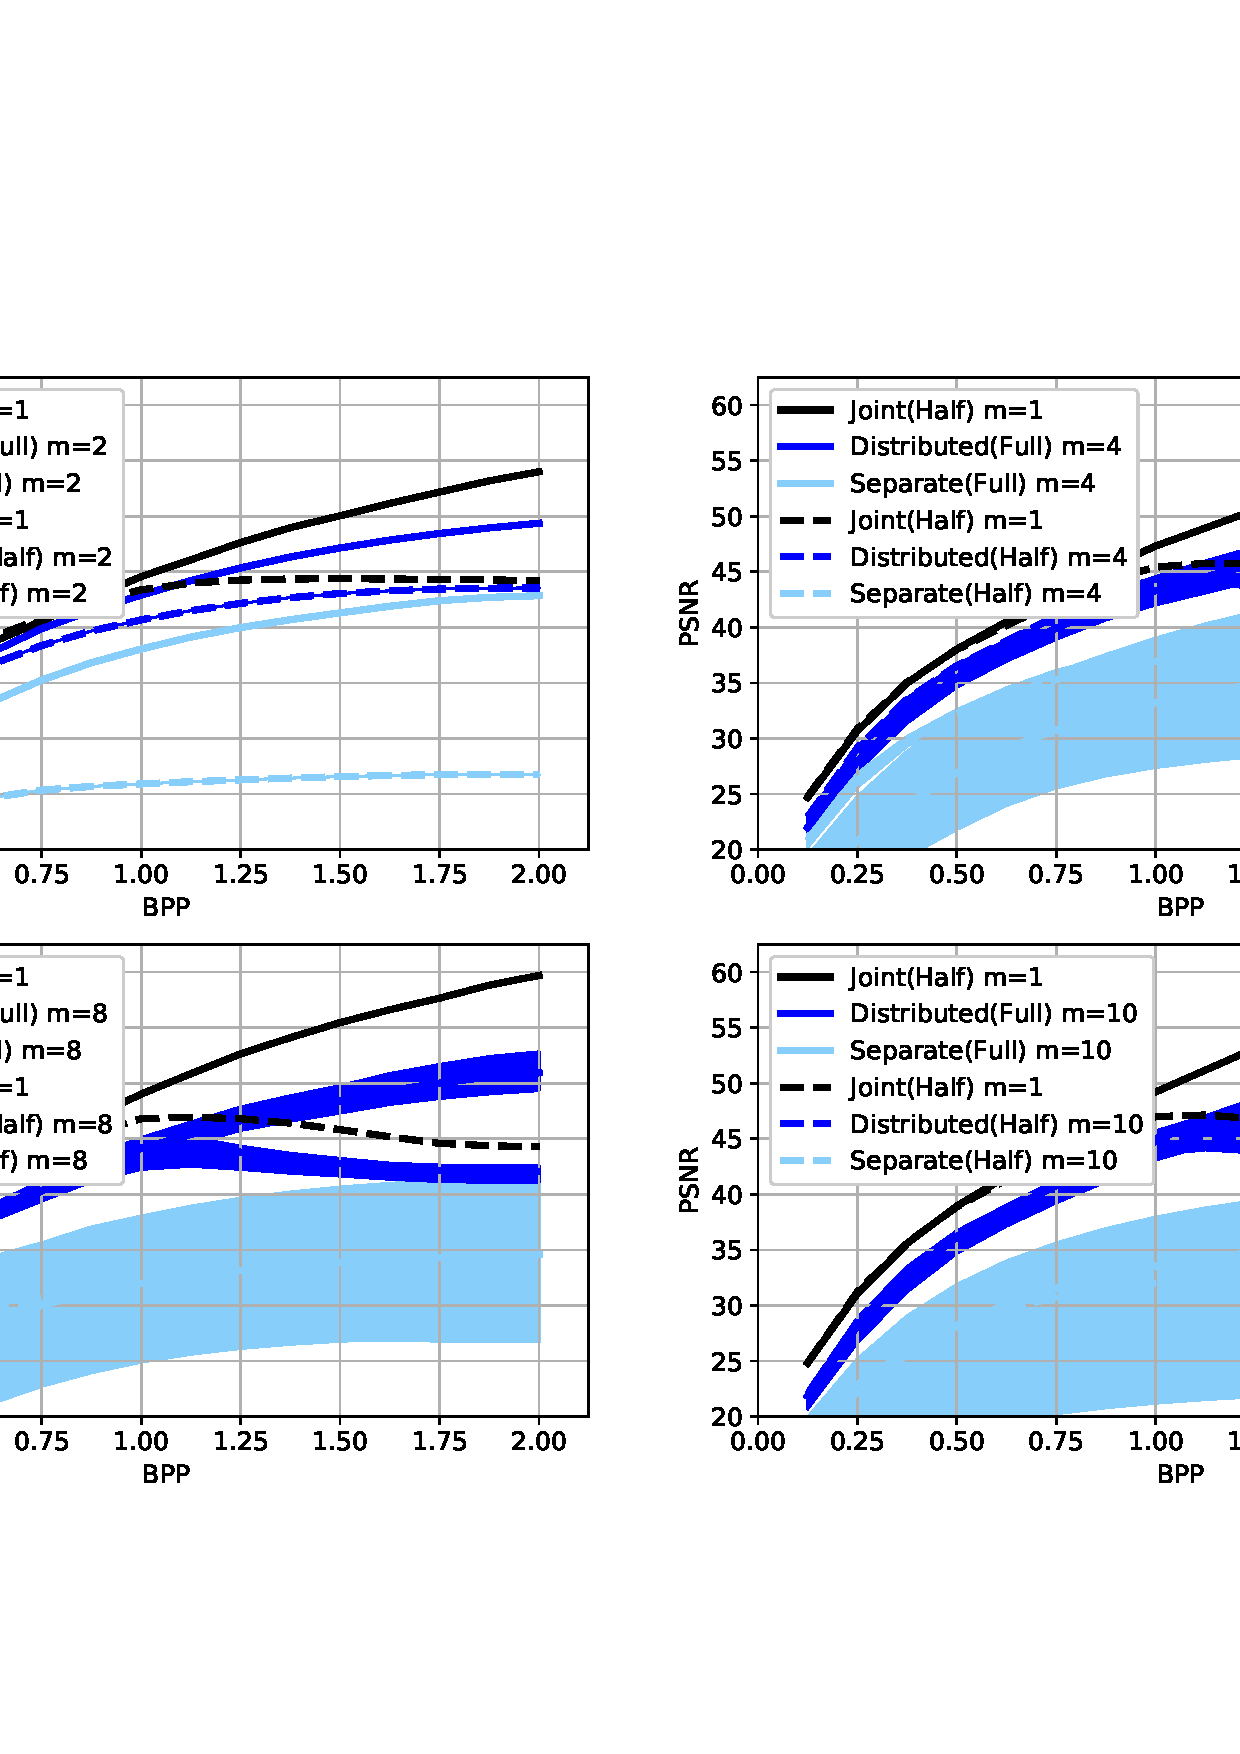
\includegraphics[width=0.8\linewidth]{half_class_band.png}
\end{center}
	\vspace{-0.2cm}
   \caption{Rate-distortion curves for data sources distributed by class labels with $T=16$ for the first half of sources and $T=8$ for the second half of sources.}
   \vspace{-0.2cm}
\label{fig_7}
\end{figure*}

\subsection{Arbitrary Correlated Sources}
To address the advantage of our DNN-based DSC framework, we first experiment distributed sources with different correlations. The distributed encoders are indexed as $1, \ldots, m$. We split data into random subsets and also split them by class labels. We show the result of data sources distributed by random subsets in Fig.~\ref{fig_4}, \ref{fig_6} and by class labels in Fig.~\ref{fig_5}, \ref{fig_7}. In the first case, each distributed encoder is trained with a subset of data and only the decoder can access the codes compressed from each data source. In the second case, we distribute data sources by class labels. For example, the $m$th encoder can only access data of digit $m-1$ and the label is $m-1$ ($m\leq 10$). %The theoretical limit in the case of $m<10$ is also obtained with data of digits with labels $<m$.

The curve of distributed encoders shows that the performance of training distributed encoders and joint decoder can be very close to the theoretical limit. As the number of encoders grows, the performance decreases a little, but still dominantly outperforms training codecs for each data source separately. From various experiments we found that the gap will become smaller when more data are available. The gap also diverges as more bits are generated. This is because the residual differences used as input at each iteration are less correlated among data sources than the original images. This experiment clearly shows that near-oracle performance can be achieved without specifically estimating the correlations among different sources, a desirable feature not enjoyed by classical DSC code design. The results show that our Deep DSC framework is able to adaptively learn arbitrary correlations among arbitrary number of data sources. 

\subsection{Low Complexity Encoding}
We also demonstrate the performance of low complexity encoders which are trained with less number of iterations. In this experiment, the first half of encoders are trained with $16$ iterations, labeled as \textit{Full}, and the second half of encoders are only trained with $8$ iterations, labeled as \textit{Half}. For example, for $m=8$, encoders $1$ to $4$ are trained with 16 iterations while encoders $5$ to $8$ are trained with 8 iterations. In Fig.~\ref{fig_6} and Fig.~\ref{fig_7}, we show the dashed lines for $T=8$ and solid lines for $T=16$ respectively. The theoretical limits (in black lines) are trained with all available data. The first half of encoders and the second half of encoders only access half of the whole dataset respectively.

Although the theoretical limits are obtained from all data, full and half complexity encoders %, only using half of the whole dataset, 
can still approach their theoretical limits (in black dash). Half complexity encoders perform as well as full complexity encoders in the first 8 iterations, because their correlations of the first eight iterations are trained properly with the model parameters. After the eighth iteration, both full and half complexity encoders can still approach their theoretical limits, because the trained correlations of residual differences from the first eight iterations can be reused at the second eight iterations without training. However, without specifically training the correlations after the eighth iterations, the performance of half complexity encoders slightly decreases when BPP is larger than 1. %a little compared to Fig.~\ref{fig_4} and \ref{fig_5}.


\subsection{Robust Distributed Encoding}
Our data-driven DSC framework, unlike classical DSC code design, does not require synchronization of data sources. In classical DSC code design, if syndrome bits $H(X|Y)$ are used and the data source $X$ is accidentally blocked, we will not be able to decode data source $Y$. As mentioned previously, we test each encoder separately with all test data once training is finished. Even only one of distributed encoders is functional, it can still benefits from its correlations with other sources because their correlations are already trained with the model parameters. 

%Our results are summarized 
%A confidence band is determined by the best and worst performance of all encoders at each iteration.
All our experiments show that distributed encoders not only dominates separately trained codecs but also have narrower confidence band. As the number of encoders increases, the confidence band of separately trained codecs becomes wider because each separate codec can only access very limited amount of data and thus suffer from overfitting. As the number of iterations increases, the confidence band also becomes wider. This is because the residual differences at later iterations become less correlated. Finally, the confidence band of data sources distributed by class labels is also wider than that of data sources distributed by random subsets. This is mainly because encoders specialize on data with the same label so their performance fluctuates more than encoders trained by data sources distributed by random subsets. %; 2 part of data sources distributed by class labels when $m<10$.
%------------------------------------------------------------------------
\section{Conclusion}
We introduce a data-driven Distributed Source Coding framework based on Deep Recurrent models. Compared to classical code design, our method has the following advantages. First, the compression quality of our recurrent model is scalable. Data sources can be efficiently compressed at different bit rates with a single recurrent model. Second, instead of explicitly estimating the correlations among data sources in advance, we use data-driven approach to learn the correlations with the neural network parameters. Therefore, given enough training data, our method can handle arbitrary number of sources with arbitrary correlations. Third, as one of the most important applications of Distributed Source Coding, low complexity encoder is also shown to be feasible based on our experimental results. Data sources trained with less data and fewer number of iterations can still approach the theoretical limit obtained when all data are used. Finally, we show the robustness of our framework. Unlike classical code design which may require careful data source synchronization, each distributed encoder of our model, once trained and deployed, can be used independently of others because the correlations are already learned by the model parameters. 

We point out two interesting directions of future work. First, training of the current architecture may be improved by introducing adaptive weights over different iterations, e.g. by using an attention mechanism. Second, the network architecture may be further extended to handle time-dependent data sources.
%We hope this work can pave a new way of practical distributed source code design.
\section*{Acknowledgement}
This work is supported by Office of Naval Research (ONR) grant numbers N00014-18-1-2244.
%------------------------------------------------------------------------
{%\small
\balance
\bibliographystyle{IEEEtran}
\documentclass[10pt,twocolumn,letterpaper]{article}

\usepackage{iccv}
\usepackage{times}
\usepackage{epsfig}
\usepackage{graphicx}
\usepackage{amsmath}
\usepackage{amssymb}
\usepackage{algorithm}
\usepackage{algorithmic}
\usepackage{balance}

% Include other packages here, before hyperref.
\usepackage{bm}

% If you comment hyperref and then uncomment it, you should delete
% egpaper.aux before re-running latex.  (Or just hit 'q' on the first latex
% run, let it finish, and you should be clear).
\usepackage[pagebackref=true,breaklinks=true,letterpaper=true,colorlinks,bookmarks=false]{hyperref}

\iccvfinalcopy % *** Uncomment this line for the final submission

\def\iccvPaperID{4386} % *** Enter the ICCV Paper ID here
\def\httilde{\mbox{\tt\raisebox{-.5ex}{\symbol{126}}}}

% Pages are numbered in submission mode, and unnumbered in camera-ready
\ificcvfinal\pagestyle{empty}\fi
\begin{document}

%%%%%%%%% TITLE
\title{Distributed Lossy Image Compression with Recurrent Networks}

\author{Enmao Diao\\
Duke University\\
{\tt\small enmao.diao@duke.edu}
% For a paper whose authors are all at the same institution,
% omit the following lines up until the closing ``}''.
% Additional authors and addresses can be added with ``\and'',
% just like the second author.
% To save space, use either the email address or home page, not both
\and
Jie Ding\\
University of Minnesota\\
{\tt\small dingj@umn.edu}
\and
Vahid Tarokh\\
Duke University\\
{\tt\small vahid.tarokh@duke.edu}
}

\maketitle
%\thispagestyle{empty}


%%%%%%%%% ABSTRACT
\begin{abstract}
We propose a new architecture for distributed image compression from a group of distributed data sources. The proposed architecture, which we refer to as symmetric Encoder-Decoder Convolutional Recurrent Neural Network, is able to significantly outperform the state-of-the-art compression techniques such as JPEG on rate-distortion curves. We also show that by training distributed encoders and joint decoders on correlated data sources, the performance of compression is much better than that by training codecs separately. For $10$ distributed sources, our distributed system remarkably performs within 2 dB peak signal-to-noise ratio (PSNR) of that of a single codec trained with all data sources. We experiment distributed sources with different correlations and show how our methodology well matches the Slepian-Wolf Theorem in Distributed Source Coding (DSC). Our method is also shown to be robust to the lack of presence of encoded data from a number of distributed sources. To the best of our knowledge, this is the first data-driven DSC framework for general distributed code design with Deep Learning.

\end{abstract}

%%%%%%%%% BODY TEXT
\section{Introduction}
It has been shown by a variety of previous works that Deep Neural Networks (DNN) can achieve comparable results as classical image compression techniques \cite{toderici2015variable,balle2016end,gregor2016towards,toderici2017full,theis2017lossy,johnston2017improved,liu2018cnn}. Most of these methods are based on autoencoder networks and quantization of bottleneck representations, e.g. by quantizing the codes into 8 bit integers and minimizing $\mathcal{L}_1$-penalized loss to sparsify the codes. These models usually rely on entropy codec to compress the sparsified codes. Moreover, to achieve different compression rates, it is unavoidable to train multiple models with different regularization parameters separately.

Among the existing literature of image compression, the recurrent neural network (RNN) based architecture \cite{toderici2015variable} is known to be the pioneering architecture that outperforms classical codecs. The model uses a recurrent autoencoder to encodes the residual difference between the original input and the reconstruction output. At each iteration, new binary coded information is extracted from the residual and the context from previous iterations is stored in the hidden state of the recurrent model. The compression rate, in this case, is varying according to the number of iterations of a single recurrent model. An improved architecture was proposed in \cite{johnston2017improved} that can simultaneously archive spatially adaptive bit rates in a single training phase. 

Motivated by various issues such as data privacy, computational cost, robustness against missing data, the following question has recently gained a lot of research interest. 

\textit{Can distributed encoders perform as well as a single encoder trained with all data sources together?} 

A positive answer from theoretical perspective was given in the context of Distributed Source Coding (DSC). 
In information theory, DSC is an important problem regarding the compression of multiple correlated data sources. The Slepian-Wolf Theorem shows that lossless coding of two or more correlated data sources with separate encoders and a joint decoder can compress data as efficiently as the optimal coding using a joint encoder and decoder \cite{slepian1973noiseless,cover1975proof}. The extension to lossy compression with Gaussian data sources was proposed as Wyner-Ziv Theorem \cite{wyner1976rate}. Although these theorems were published in 1970s, it was after about 30 years that practical applications such as Distributed Source Coding Using Syndromes (DISCUS) emerged \cite{pradhan2003distributed}. One of the main advantages of DSC is that the computation complexity of the encoder is shifted to the decoder. Typically, low complexity encoders can be used in multi-view video coding and sensor networks \cite{girod2005distributed,xiong2004distributed}. 
Motivated by the theoretical development of DSC, in this work we propose a DNN architecture that consists of distributed encoders and a joint decoder. We show that distributed encoders can perform as well as a single encoder trained with all data sources together.
Our proposed DSC framework is data-driven by nature, and it can be applied to distributed data even with unknown correlation structure.

\begin{figure}
\begin{center}
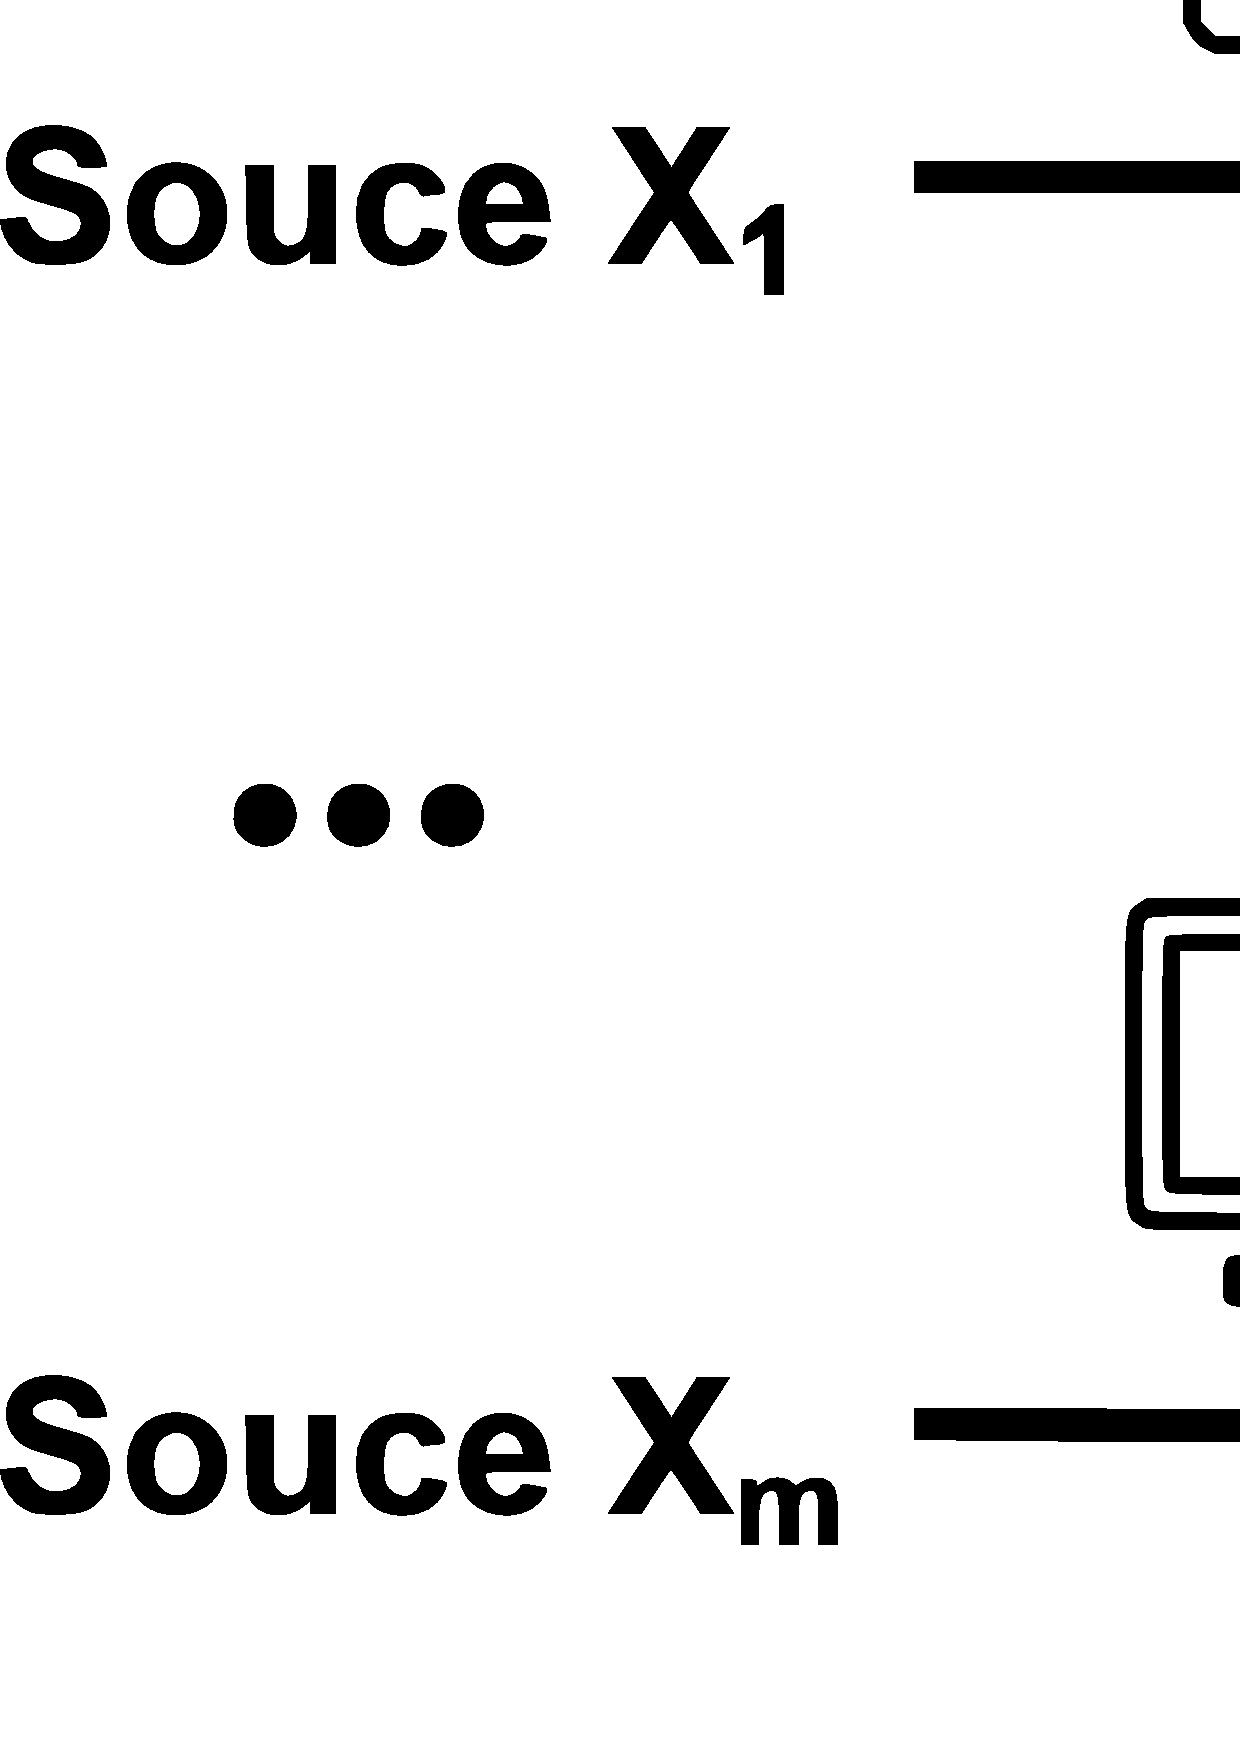
\includegraphics[width=1\linewidth]{DeepDSC.pdf}
\end{center}
   \caption{Illustration of Deep Distributed Source Coding.}
\label{fig_0}
\end{figure}

\begin{figure*}
\begin{center}
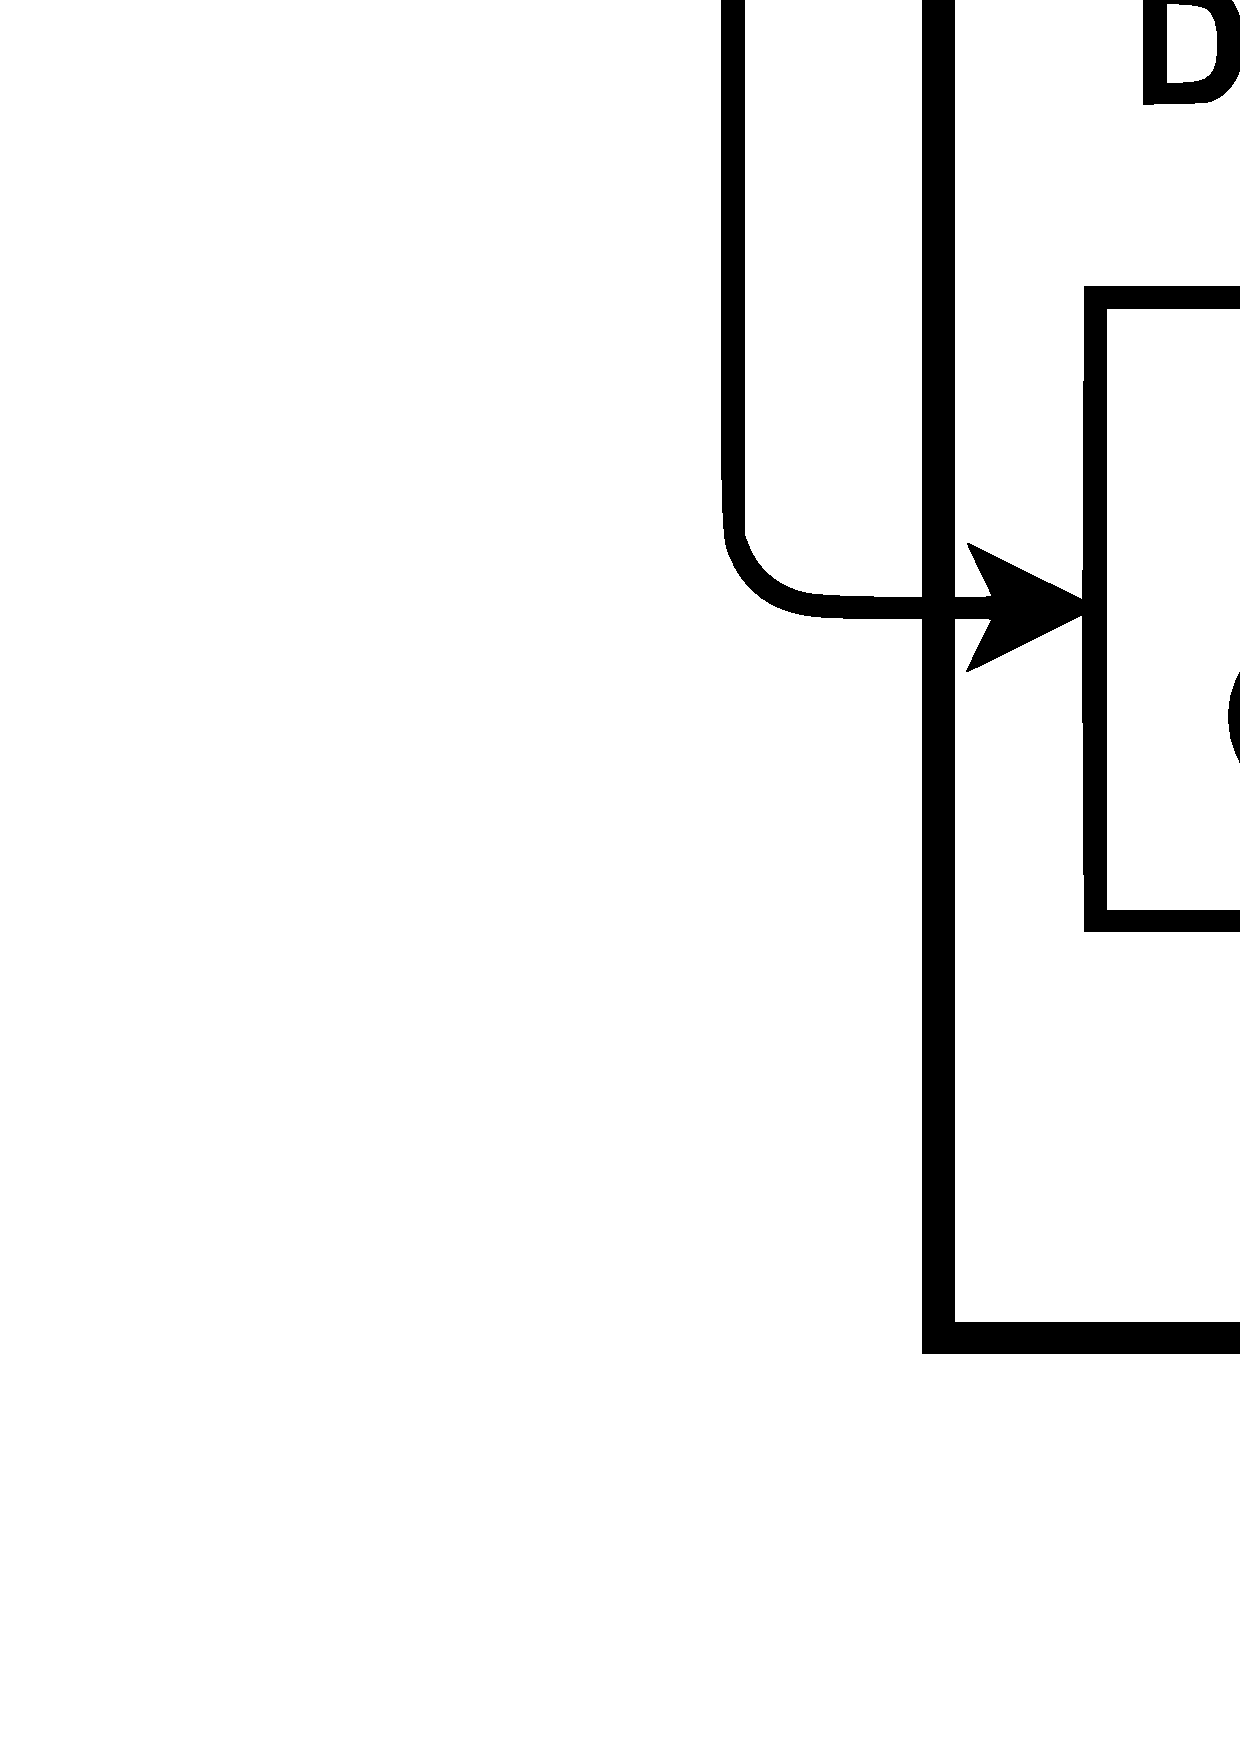
\includegraphics[width=0.8\linewidth]{DeepEncoderDecoder.pdf}
\end{center}
   \caption{Illustration of pixel-shuffled symmetric Encoder-Decoder architecture.}
\label{fig_1}
\end{figure*}
The advantages of our proposed architecture (illustrated in Fig.~\ref{fig_0} and \ref{fig_1}) are fourfold. 
First, the architecture is naturally scalable in the sense that codes can be decoded at more than one compression quality levels, and it allows efficient coding of correlated sources which are not physically co-located. This is especially attractive in video streaming applications \cite{guillemot2007distributed,gehrig2008distributed}. Second, unlike classical DSC which requires customized code design for different scenarios \cite{xiong2004distributed}, data-driven DSC framework can handle nontrivial distribution of image sources with arbitrary correlations. Third, the computation complexity of the encoder can be transferred to the decoder, a system of low complexity encoders can be used in a variety of application domains, such as multi-view video coding \cite{girod2005distributed}, sensor networks \cite{xiong2004distributed}, and under-water image processing where communication bandwidth and computational power are quite restricted \cite{stojanovic2009underwater,schettini2010underwater}. Fourth, the distributed framework can be more robust against heterogeneous noises or malfunctions of encoders, and such robustness can be crucial in, e.g., unreliable sensor networks \cite{girod2005distributed,ishwar2005rate,xiao2006distributed}.

The paper is outlined below. We review previous related work in Section 2 and describe our proposed method in details in Section 3. We describe our architecture for general image compression and its base modules in Section 3.1-3.4. Then we elaborate the Deep Distributed Source Coding framework in Section 3.5. Experimental results are shown in Section 4, followed by conclusions in Section 5.

%------------------------------------------------------------------------
\section{Related Work}
Though there has been a variety of research on lossy data compression in the past few decades, little attention has been paid to a systematic approach for general and practical distributed code design, especially in the presence of an arbitrary number of nontrivial data sources with arbitrary correlation %and possibly sources and correlation with memory. 
\cite{xiong2004distributed}. 
A main motivation of this work is to attempt to replace the practical hand-crafted code design with data-driven approaches. 
To our best knowledge, what we propose is the first data-driven DSC architecture. 
Unlike hand-crafted quantizers, our neural network-based quantizers show that the correlations among different data sources can be trained by the model parameters. We empirically show that the Slepian-Wolf limit can be achieved with our methodology. 

\subsection{Image compression with Deep Learning}
There exist a variety of classical codecs for lossy image compression. Although the JPEG standard \cite{wallace1992jpeg} was developed thirty years ago, it is still the most widely used image compression method. Several extensions to JPEG including JPEG2000 \cite{skodras2001jpeg}, WebP \cite{google2010webp} and BPG \cite{bellard2014bpg} have been developed. Most of these classical codecs rely on a quantization matrix applied to the coefficients of discrete cosine transform or wavelet transform.

The standard methods of compression with deep learning roughly fall into two categories. Non-recurrent autoencoders which rely on $\mathcal{L}_1$ penalty to sparsify the 8-bit integer codes, and recurrent models which introduce binary codes at each iteration. 
%Autoencoders are widely used as a general framework for neural network-based image compression. Bottleneck representations are quantized into 8-bit integers or binaries. 
The compression rate of non-recurrent models is not scalable and their performance heavily rely on the sparsity which entropy codec can take advantage of. 
Another challenge is to well define the derivative of quantizations of bottleneck representations. Ball\'e et al. \cite{balle2016end} replaced non-differentiable quantization step with a continuous relaxation by adding uniform noises. Toderici \cite{toderici2015variable}, on the other hand, used a stochastic form of binarization. 
The recurrent model~\cite{toderici2015variable,johnston2017improved}, on the other hand, has scalable compression rates. It generates more codes when the residual difference between the input and output of the model is compressed again.

\subsection{Distributed Source Coding}

\begin{figure}[t]
\begin{center}
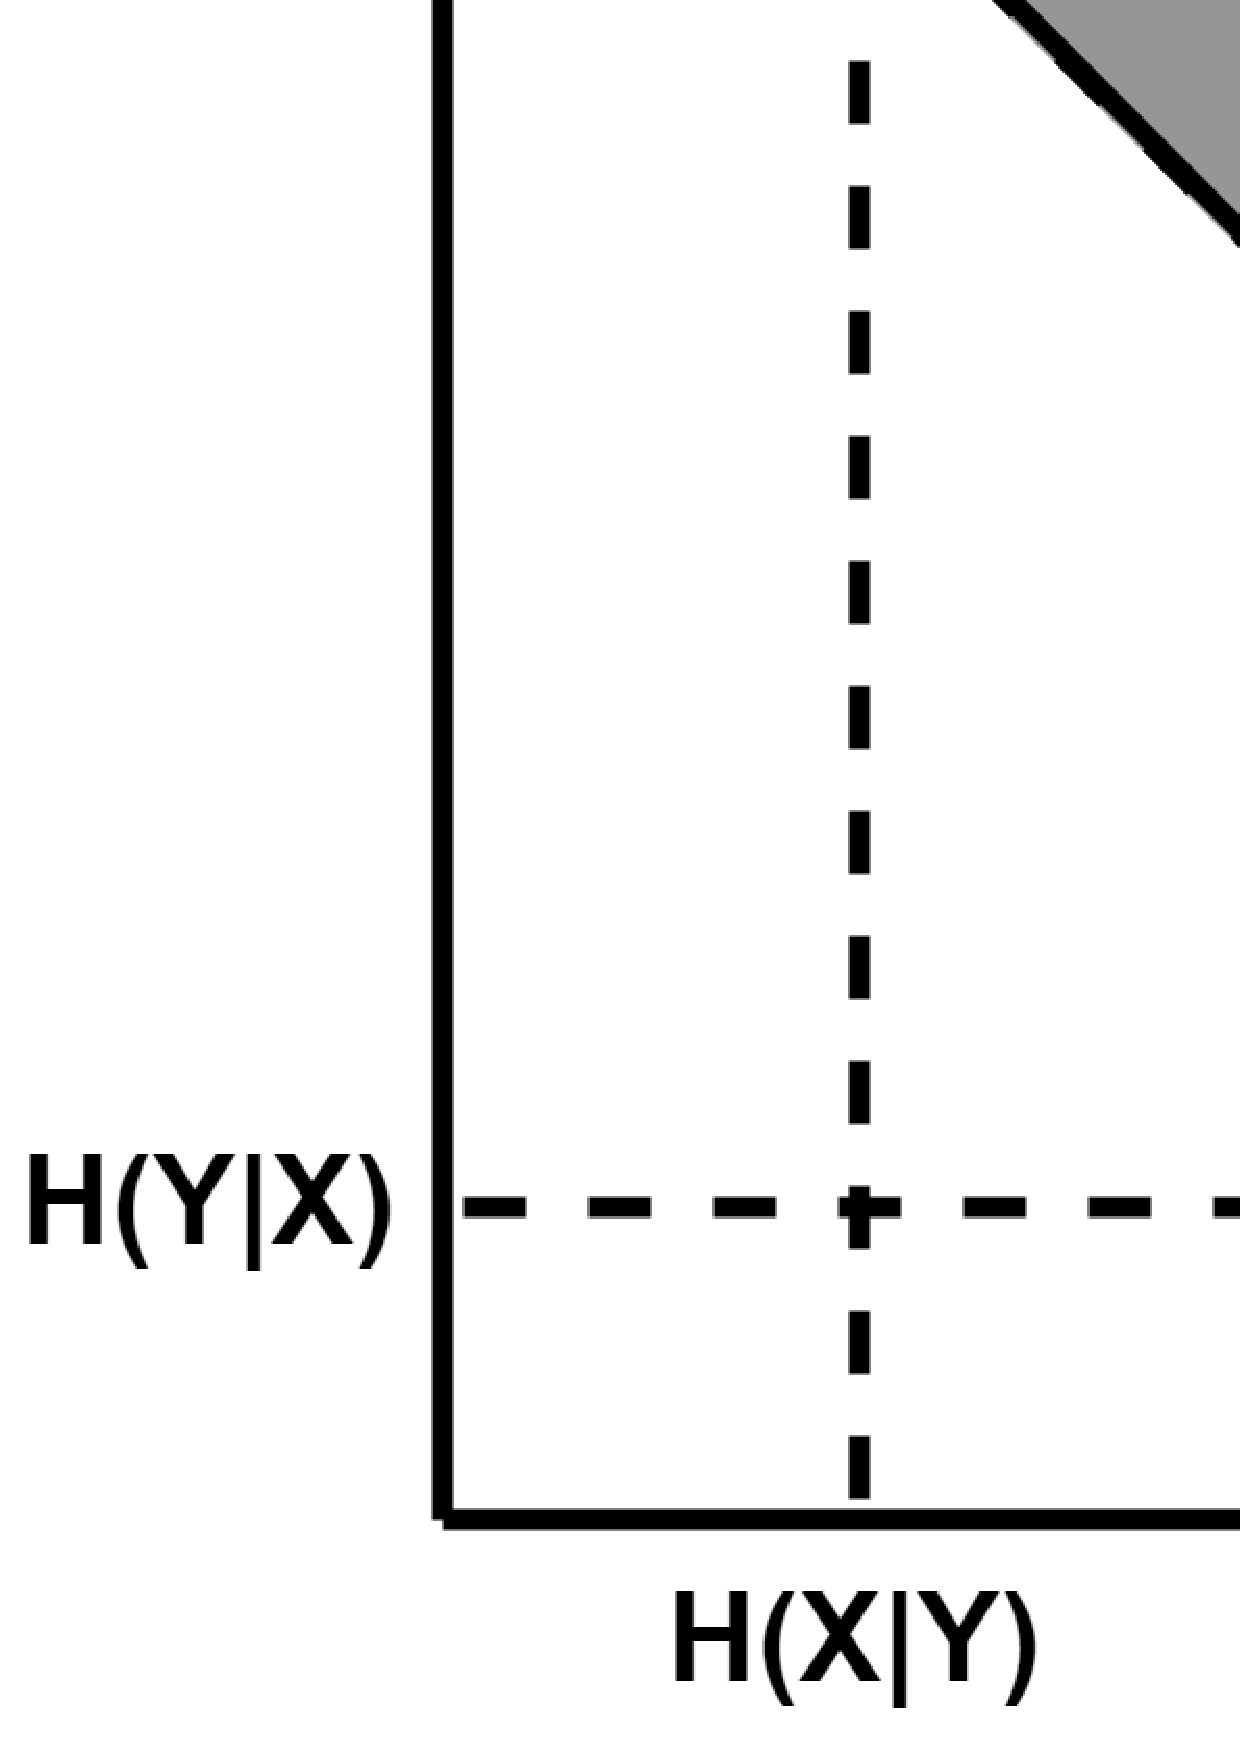
\includegraphics[width=0.8\linewidth]{SlepianWolf.pdf}
\end{center}
   \caption{The Slepian-Wolf achievable region for two sources $X$ and $Y$.}
\label{fig_2}
\end{figure}
Our methodology is deeply rooted in information-theoretic results on DSC which have been established since 1970s. The Slepian-Wolf \cite{slepian1973noiseless} Theorem shows that two correlated data sources encoded separately and decoded jointly can perform as well as joint encoding and decoding, and outperform separate encoding and separate decoding. The striking result indicates that as long as the codes are jointly decoded, there can be no loss in coding efficiency even the codes are separately encoded. Cover \cite{cover1975proof} generalizes the achievability of Slepian-Wolf coding to arbitrary number of correlated sources. Wyner-Ziv Coding \cite{wyner1976rate} gives a rate-distortion curve as an extension to lossy cases.

A classical illustration of Slepian-Wolf achievable region is shown in Fig.~\ref{fig_2}. We can achieve the performance of joint encoding and decoding of two data sources $X$ and $Y$ where the bit rate $R$ is equal to the joint entropy $H(X,Y)$ with separate encoding and joint decoding. Specifically, the achievable region proved by the Slepian-Wolf Theorem is given by $R_X\geq H(X|Y),R_Y\geq H(Y|X),$ and $R_X+R_Y\geq H(X,Y)$ as shown in the shaded area of Fig.~\ref{fig_2}. Here $R_{\cdot},H(\cdot)$ denote the bit rates and (conditional) entropies in classical Shannon theory. In practice, although some works are proposed to approach the mid-point $C$ \cite{schonberg2004distributed}, the most widely used scheme is source coding with side information (syndrome bits) at the decoder \cite{pradhan2003distributed}. This code design takes advantage of the corner points $A$ and $B$ which correspond to $R(X,Y) = R(Y)+R(X|Y)$ and $R(X,Y) = R(X)+R(Y|X)$ respectively. As an example, two 8-bit grayscale images $X$ and $Y$ have pixel values at the same location with (nonlinear) correlation implicitly determined by $x \in \{y-4, y-3, y-2, y-1, y, y+1, y+2, y+3\}$. Instead of sending 16 bits, we can send bits with $R=H(Y)+H(X|Y)$. We can take modulo of $x-y$ with respect to $8$ which only requires a 3-bit codebook $\tilde{x} \in \{4, 5, 6, 7, 0, 1, 2, 3\}$. Specifically, for $x=124$ and $y=128$, we transmit $\tilde{x}=(x-y) \mod 8$ which is 4 and $y=128$. The joint decoder will decode $x$ based on $y$ as $x = y-4 = 124$.

Some researchers have also shown the applicability of DSC on still images \cite{dikici2005distributed}. In practical applications, low complexity video encoding benefits from the DSC framework which can transfer the complexity of encoder to decoder \cite{puri2002prism,aaron2002wyner}. Scalable Video Coding can also be incorporated with DSC \cite{xu2006layered}. These proposed methods indicate the feasibility of DSC in our problem setting.

%-------------------------------------------------------------------------
\section{Methods}
In this section, we first describe the symmetric Encoder-Decoder architecture used in our research work. We will elaborate the base modules including Convolutional Long short-term memory (ConvLSTM), Pixel (Un)Shuffle, and Binarizer used in our model. We will then describe how this Deep Learning architecture is used in Distributed Source Coding framework.

\subsection{Network Architecture}
Our compression network consists of an encoder, a binarizer, and a decoder. The activation function following each Convolutional Neural Network (CNN) module is $\tanh$. For the first iteration of our model, the input images are initially encoded and transformed into $(-1,1)$ by $\tanh$ activation function. Binary codes are quantized from transformed bottleneck representations. The decoder then reconstructs images based on the received binary codes. Finally, we compute the residual difference between the original input images and the reconstructed output images. At the next iteration, the residual difference is feedback as the new input for our model. This procedure is repeated multiple iterations to gain more codes for better reconstruction performance. Therefore, the reconstructed images at each iteration are the sum of output reconstructions from previous and current iterations.

Consider dataset $X = \{x\}^{N}$ consisting of $N$ i.i.d. samples of some continuous or discrete variables $x$. The data generating process is unknown. Autoencoders for compression and reconstruction can be formulated in the following way. Data can be compressed with a neural network-based encoder $f(x;\theta)$ into quantized codes $\tilde{z}$ and reconstructed with a decoder $g(\tilde{z};\phi)$. We can binarize bottleneck representations $z$ and control the compression quality by varying its channel sizes. The loss function $\mathcal{L}(x,\tilde{x})$ is minimized with respect to the model parameters $\theta$ and $\phi$.
\begin{align}
z &= f(x;\theta),\\
\tilde{z} &= \text{Binarize}(z),\\
\tilde{x} &= g(\tilde{z};\phi),\\
\text{Minimize } \mathcal{L}&(x,\tilde{x})
\end{align}
Deep recurrent autoencoder gradually increases compression quality by creating a correlated residual sequence from the difference between the input and output of our model. The advantage of recurrent model is that we can train one model with scalable compression quality. Classical autoencoders, on the contrary, have to train multiple networks with different penalty coefficients or channel sizes for different compression qualities. Suppose $T$ iterations are used, we can formulate the recurrent autoencoder in the following way.
\begin{align}
z_t &= f(x_t;\theta),\\
\tilde{z}_t &= \text{Binarize}(z_t),\\
\tilde{x}_t &= g(\tilde{z}_t;\phi),\\
x_{t+1} &= x_t-\tilde{x}_t\text{, }\tilde{x}_1=0,\\
\text{Minimize } \frac{1}{T}&\sum_{t=1}^{T}\mathcal{L}(x_1,\sum_{i=1}^{t}\tilde{x}_i).
\end{align}
In the recurrent autoencoder, the compression quality is controlled by several factors including the scale factor of Pixel (Un)Shuffle module $r$, the depth of model $D$, the channel size of bottleneck representations $C$, and the number of iterations $T$. The height and width of bottleneck representations are determined by $T$ and $D$. As we have $N$ batch images with shape $H,W$, the size of codes after $T$ iterations is $(N,T,C,H/(r^D),W/(r^D))$. For example, with $r=2$, $D=3$, and $C=2^D$, one $32 \times 32$ RGB image will generate $(1,1,8,4,4)$ binary codes for a single iteration. Thus, we will add up $\frac{8
\times4\times4}{32\times32} = 0.125$ Bit Per Pixel (BPP) for this iteration. Although we configure these hyper-parameters, we believe it is possible to train these configurations in future works.

\subsection{Convolutional Long short-term memory}
As proposed by \cite{xingjian2015convolutional}, simply replacing the Fully Connected (FC) layer in LSTM with convolutional layer, ConvLSTM is able to capture spatial structure in the temporal sequence. We do not add any bias term to our modules because the output of each layer is saturated by $\tanh$. The key equations are shown below.
\begin{align}
i_t &= \sigma(W_{xi}*x_t + W_{hi}*h_{t-1}) ,\\
f_t &= \sigma(W_{xf}*x_t + W_{hf}*h_{t-1}) ,\\
c_t &= f_tc_{t-1}+i_t\tanh(W_{xc}*x_t + W_{hc}*h_{t-1}), \\
o_t &= \sigma(W_{xo}*x_t + W_{ho}*h_{t-1}) ,\\
h_t &= o_t\tanh(c_t).
\end{align}
The first and last layers of the encoder and decoder are feed-forward Convolutional Neural Network with $\tanh$ activations. The recurrent layers are all ConvLSTM networks. We do not replace CNN layer with ConvLSTM because the size of the feature maps of hidden state at shallow layers cost a mass amount of memory. From our various experimental studies, the performance does not degrade significantly either because no convolutional layers are in between ConvLSTM layers.

\subsection{Pixel (Un)Shuffle}
We resize feature maps with Pixel (Un)Shuffle modules. Pixel Shuffle module is originally proposed by \cite{shi2016real} to tackle image and video super-resolution problem. Compared to bilinear interpolation and tranposed convolutional layers, Pixel Shuffle module is much more computationally efficient, because it is non-parametric and only requires tensor reshaping and dimension permutation. We note that although this method is widely used for upscaling, it is actually invertible and we propose to use its inversion for downscaling. Thus, the encoder and decoder can be constructed symmetrically. Our experimental results show that symmetric Encoder-Decoder architecture actually produces much better results with less number of parameters, compared to the asymmetric architecture as proposed in \cite{toderici2017full}. We describe these two modules with the following pseudocodes \ref{alg_0} and \ref{alg_1}.

\begin{algorithm}
\caption{Pixel UnShuffle}
\begin{algorithmic}
\label{alg_0}
\REQUIRE $X\sim(N,C,H,W)$, $r_H,r_W$
\ENSURE $r_H,r_W$ are integers, divides $H,W$
\STATE Reshape $X\sim(N,C,H/r_H,r_H,W/r_W,r_W)$
\STATE Permute $X\sim(N,C,r_H,r_W,H/r_H,W/r_W)$
\STATE Reshape $X\sim(N,C\times r_H\times r_W,H/r_H,W/r_W)$
\end{algorithmic}
\end{algorithm}

\begin{algorithm}
\caption{Pixel Shuffle}
\begin{algorithmic}
\label{alg_1}
\REQUIRE $X\sim(N,C,H,W)$, $r_H,r_W$
\ENSURE $r_H,r_W$ are integers, $r_H\times r_W$ divides $C$
\STATE Reshape $X\sim(N,C/(r_H \times r_W),r_H,r_W,H,W)$
\STATE Permute $X\sim(N,C/(r_H \times r_W),H,r_H,W,r_W)$
\STATE Reshape $X\sim(N,C/(r_H \times r_W),H \times r_H,W \times r_W)$
\end{algorithmic}
\end{algorithm}

\subsection{Binarizer}
The derivative of quantization function is only defined at the rounded integer itself. Therefore, we have to replace its derivative in the backward pass of backpropagation with a form of smooth approximation \cite{rumelhart1988learning}. Thanks to a thorough discussion of different alternative approaches by \cite{theis2017lossy}, we choose to use identity function to replace its derivatives that cannot be well defined as shown in \ref{eq_15}. During training, we use a stochastic form of binarization proposed by \cite{toderici2017full}. For bottleneck representations $z \in (-1,1)$, the details of binarizer $\tilde{z}=\text{Binarize}(z)$ are described as follows, where $W_{\cdot}$ denote the standard parameter matrices between two network layers.
\begin{align}
\intertext{\textbf{Train}}
\tilde{z}=\text{Binarize}(z) &= 
    \begin{cases}
      1, &  \text{with probability } (z+1)/2\\
      -1, & \text{otherwise}
      \end{cases} \nonumber \\
\frac{d}{dz}\tilde{z} &:= \frac{d}{dz}\mathbb{E} (\tilde{z}) =  \frac{d}{dz}\mathbb{E} (z) = 1\label{eq_15}
\intertext{\textbf{Test}}
\text{Binarize}(z) &= 
    \begin{cases}
      1, & \text{if } z\geq0 \\
      -1, & \text{otherwise}
      \end{cases}
\end{align}

\subsection{Deep Distributed Source Coding Framework}
Fig.~\ref{fig_0} and \ref{fig_1} illustrates our Deep DSC coding framework. Similar to classical DSC framework, each data source is encoded separately and decoded jointly. Traditionally, researchers have to design different kind of codes for specific scenarios \cite{schonberg2004distributed}. We propose to use data-driven approach to handle complex scenarios where the distribution of data sources are unknown and their correlations can be arbitrary. Our proposal may also shed new light on sophisticated application scenarios such as videos where data sources and correlations are time dependent.

In our neural network-based DSC, %the whole encoding and decoding procedure are trained jointly. 
$M$ distributed encoders encode corresponding data sources $x^m$ that can be arbitrarily correlated. Each neural network-based encoder $f(x^m;\theta^m)$ has their own model parameters $\theta^m$. After binarizing bottleneck representations $z^m$, code sources $\tilde{z}^m$ are transmitted and concatenated batch-wisely. A single decoder $g(\tilde{z}^m;\phi)$ reconstructs images $\tilde{x}^m$ from all sources with the same model parameters $\phi$. 
In particular, the parameters of the following model are optimized with backward propagation \cite{rumelhart1988learning}. 
\begin{align}
z_t^m &= f(x_t^m;\theta^m),\\
\tilde{z}_t^m &= \text{Binarize}(z_t^m),\\
\tilde{x}_t^{m} &= g(\tilde{z}_t^{m};\bm{\phi}),\\
x_{t+1}^{m} &= x_t^{m}-\tilde{x}_t^{m}\text{, }\tilde{x}_1^{m}=0,
\end{align}
\begin{align}
\text{Minimize } \frac{1}{MT}&\sum_{t=1}^{T}\sum_{m=1}^{M}\mathcal{L}(x_1^m,\sum_{i=1}^{t}\tilde{x}_i^m).
\end{align}
Our result shows that the resulting distributed model can perform as well as encoding all data by one single encoder. However, if we encode and decode each data source separately, the performance becomes significantly worse. Moreover, correlations among data sources cannot be learned with separate parameters of decoders, i.e. with 
$\tilde{x}_t^{m} = g(\tilde{z}_t^{m};\bm{\phi^m})$.
%------------------------------------------------------------------------
\section{Experiments}
We use MNIST dataset \cite{lecun1998gradient} consisting of 60,000 training and 10,000 testing grayscale handwritten digit images. The digits have been resized from $28 \times 28$ to $32 \times 32$. The Adam optimizer \cite{kingma2014adam} is used with $\epsilon = 1e-8$, $\beta_1 = 0.9$ and $\beta_2 = 0.999$. We train model with $\mathcal{L}_1$ loss, batch size $N=100$ and learning rate $0.001$ for a total of 200 epochs. We start to decay learning rate by half at the 70th epoch and at every 20 epochs thereafter.

As described in section 3.1, we set the scaling factor for Pixel (Un)Shuffle module to be $r=2$, depth of model $D=3$, and code channel size $C=2^D$. For $T=16$, one minibatch of grayscale images with shape $(100,1,32,32)$ will be encoded to be a $(100,16,8,4,4)$ binary tensor. We evaluate all models with the metric Peak Signal to Noise Ratio (PSNR) against the Bit Per Pixel (BPP).

\begin{figure}[t]
\begin{center}
\includegraphics[width=0.8\linewidth]{codec.pdf}
\end{center}
	\vspace{-0.2cm}
   \caption{Our symmetric pixel-shuffled Encoder-Decoder outperforms classical codecs and baseline neural network-based codecs.}
   \vspace{-0.2cm}
\label{fig_3}
\end{figure}

We compare our model to the baseline model \cite{toderici2017full} and classical codecs like JPEG~\cite{wallace1992jpeg}, JPEG2000~\cite{skodras2001jpeg} and BPG~\cite{bellard2014bpg}. To directly compare the performance of network architecture, we ignore some techniques introduced by \cite{toderici2017full} and \cite{johnston2017improved} such as progressive entropy coding and hidden-state priming. Instead of bilinear interpolation or convolutional layers used in previous works\cite{toderici2017full,theis2017lossy,johnston2017improved}, our network architecture uses Pixel Shuffle in the Encoder. As a result, our network architecture has a symmetric Encoder-Decoder structure and also few number of parameters. Fig.~\ref{fig_3} shows that our symmetric pixel-shuffled Encoder-Decoder architecture outperforms classical codecs and baseline neural network-based codecs.

We run experiments with $(2,4,8,10)$ number of distributed sources. Each encoder encodes data from each data source without communicating with other encoders. The decoder jointly decodes the codes gathered from each distributed encoder. First, we compare our result, labeled as \textit{Distributed}, to the case where all data are trained with one encoder and one decoder jointly, labeled as \textit{Joint}. The `Joint' curve is approximated as the theoretical upper bound of performance. %theoretical upper bound $H(X,Y)$. 
Second, we compare our result to the case where each data source is trained with a separate pair of encoder and decoder, labeled as \textit{Separate}. We test each distributed encoder separately with all test data. The solid curves are the average performance across all encoders. At each iteration, the confidence band is determined by the best and worst performance of all encoders. 

Our experimental studies in the following sections consist of three aspects. We first experiment data sources with different correlations. We then show the performance of low complexity encoders which are trained with less number of iterations. Finally, we show the robustness of our distributed framework in the absence of a number of distributed sources.

\begin{figure*}
\begin{center}
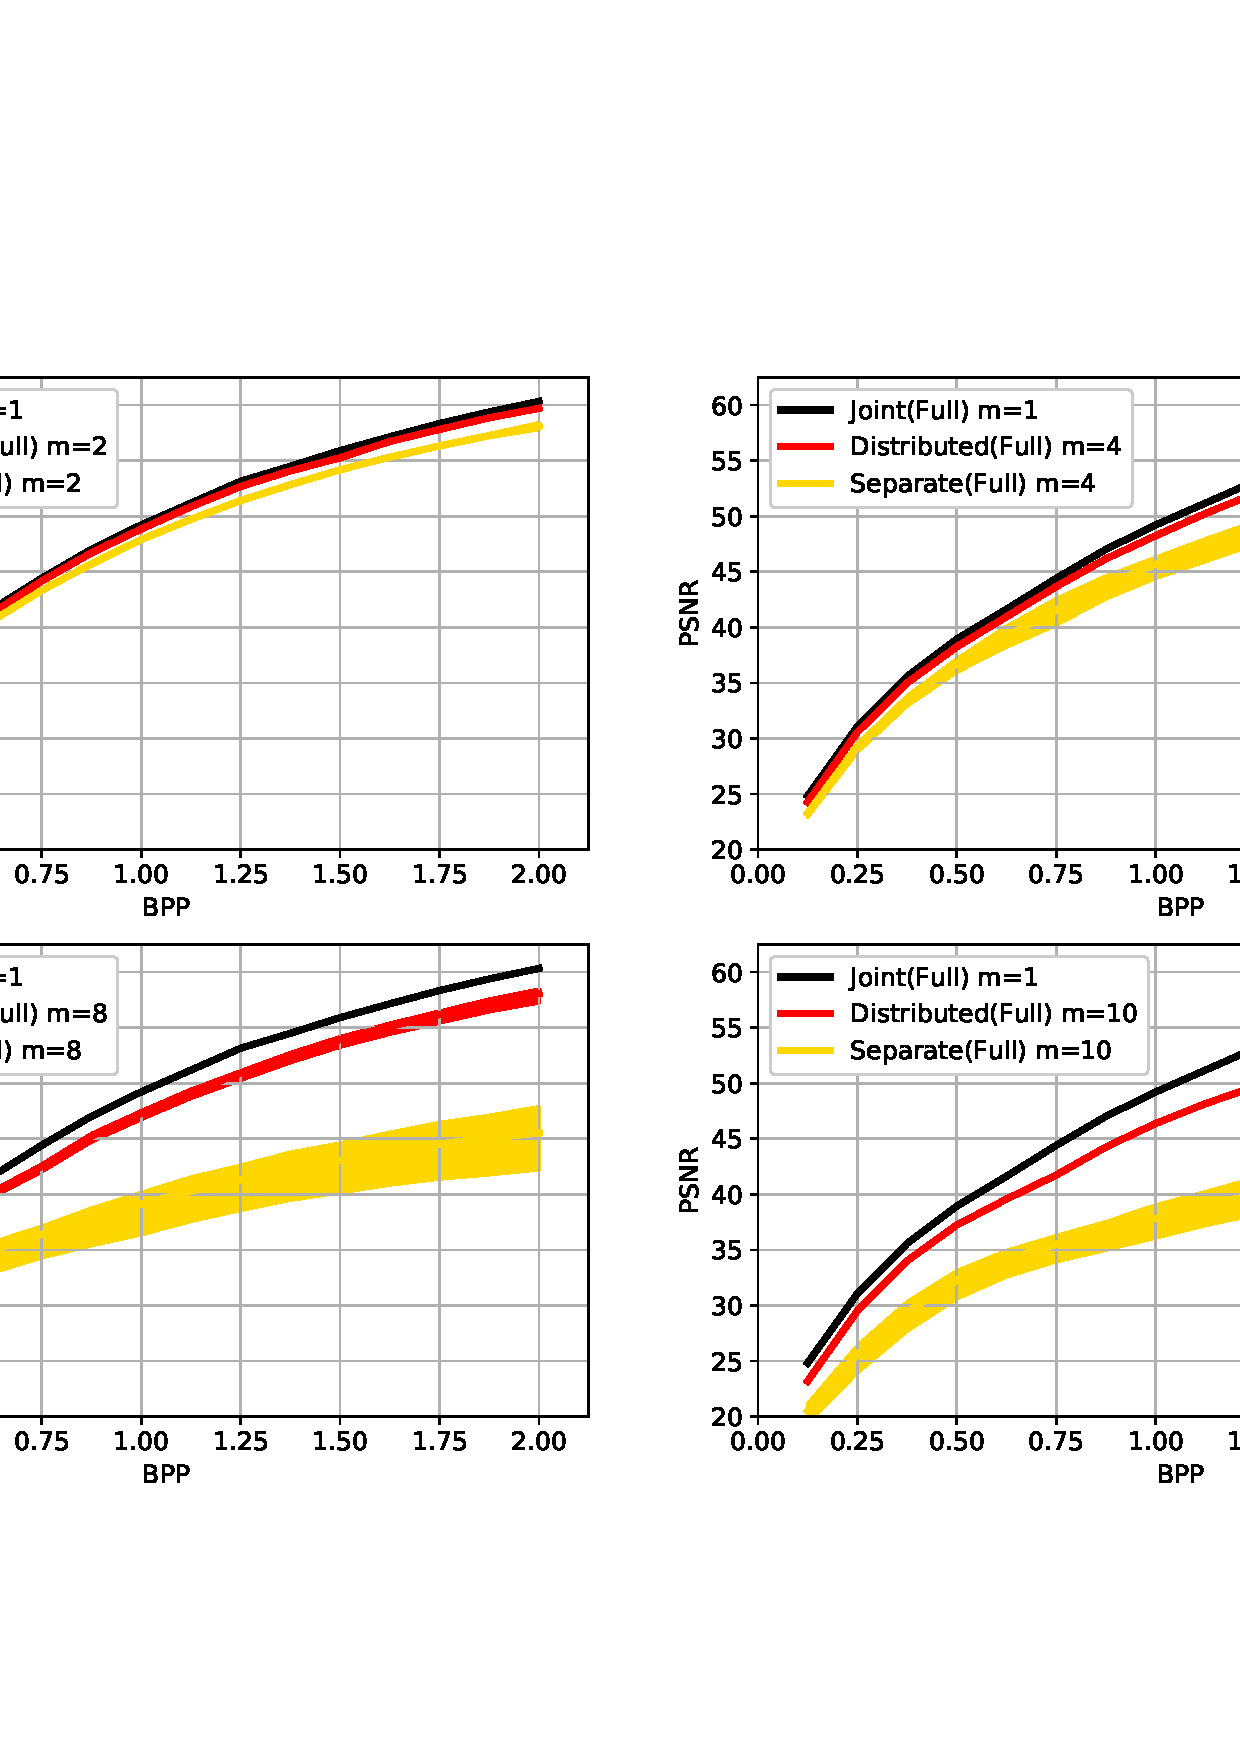
\includegraphics[width=0.8\linewidth]{full_subset_band.png}
\end{center}
	\vspace{-0.2cm}
   \caption{Rate-distortion curves for data sources distributed by random subsets with $T=16$ for all sources.}
   \vspace{-0.2cm}
\label{fig_4}
\end{figure*}

\begin{figure*}
\begin{center}
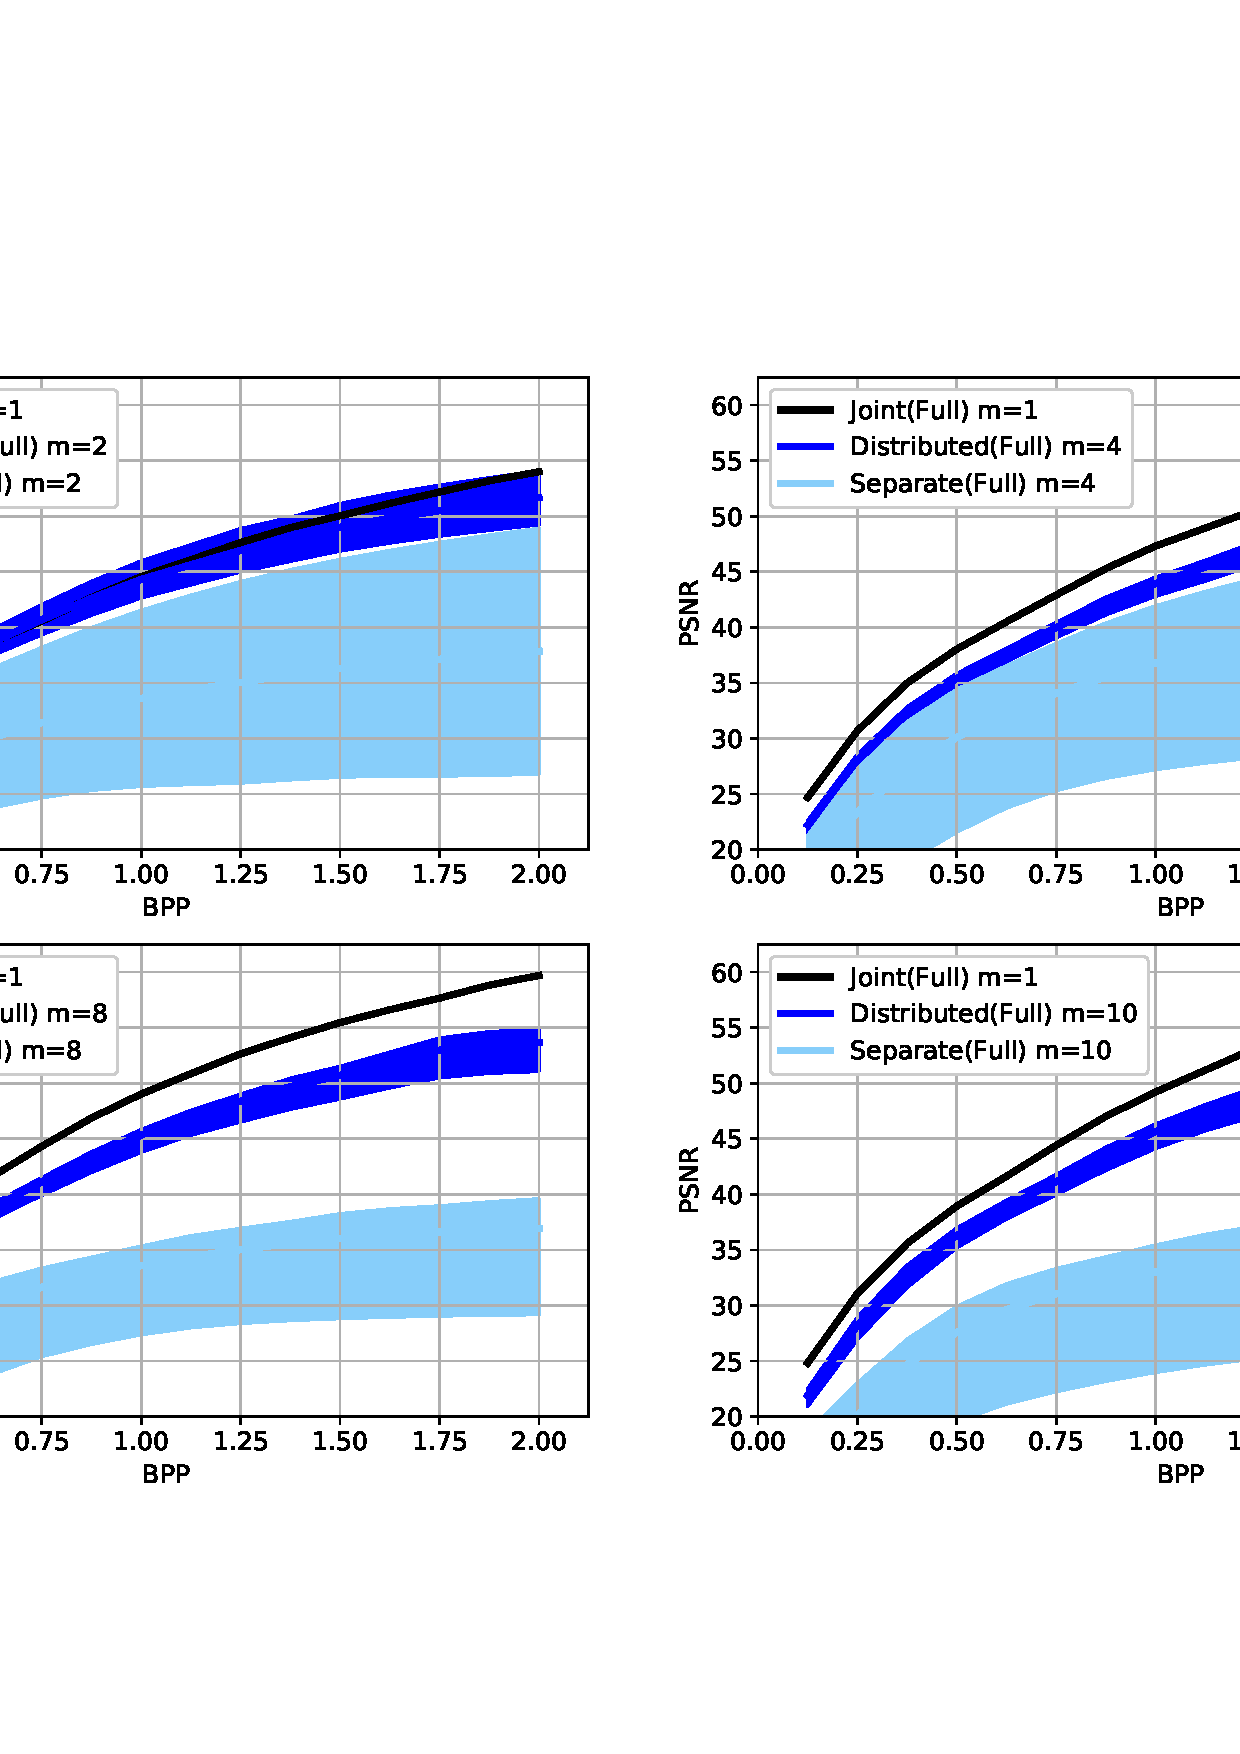
\includegraphics[width=0.8\linewidth]{full_class_band.png}
\end{center}
	\vspace{-0.2cm}
   \caption{Rate-distortion curves for data sources distributed by class labels with $T=16$ for all sources.}
   \vspace{-0.2cm}
\label{fig_5}
\end{figure*}

\begin{figure*}
\begin{center}
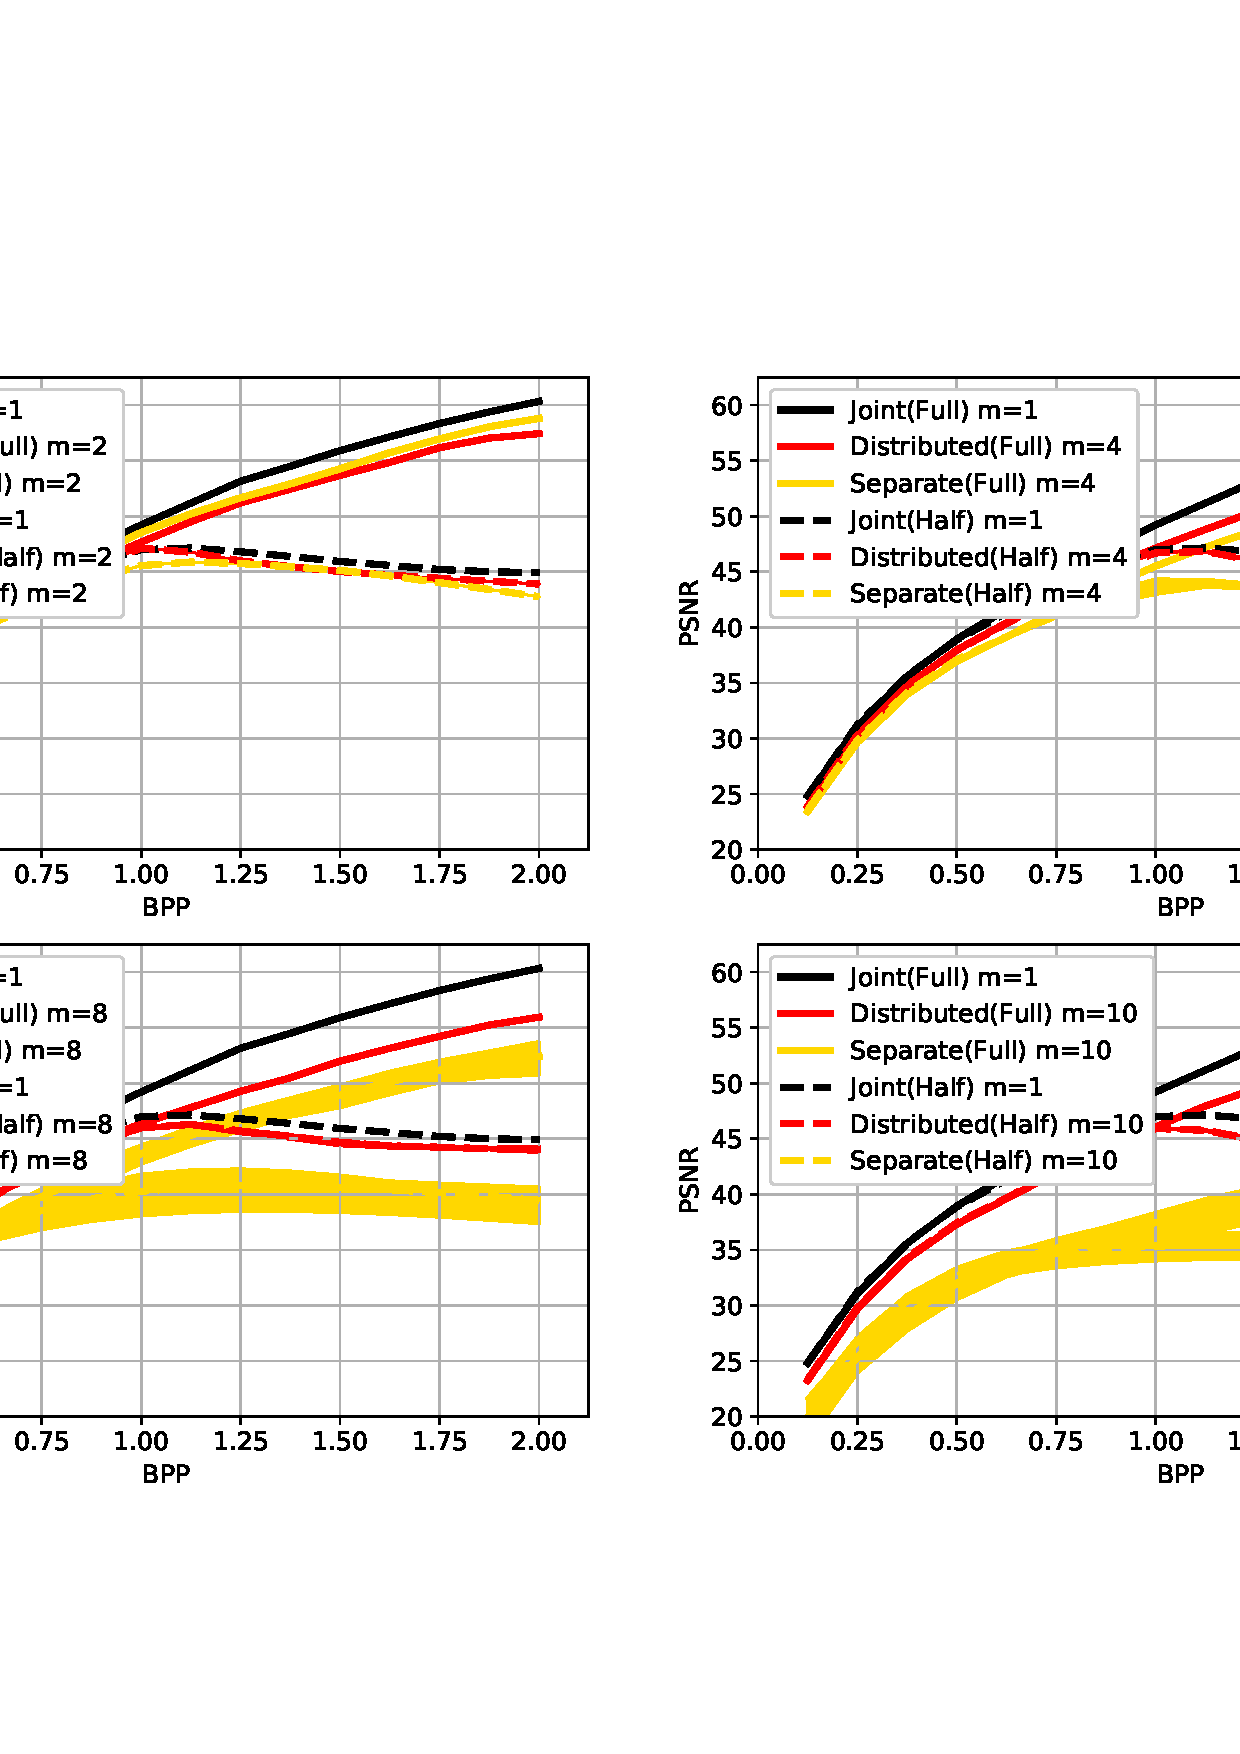
\includegraphics[width=0.8\linewidth]{half_subset_band.png}
\end{center}
	\vspace{-0.2cm}
   \caption{Rate-distortion curves for data sources distributed by random subsets with $T=16$ for the first half of sources and $T=8$ for the second half of sources.}
   \vspace{-0.2cm}
\label{fig_6}
\end{figure*}

\begin{figure*}
\begin{center}
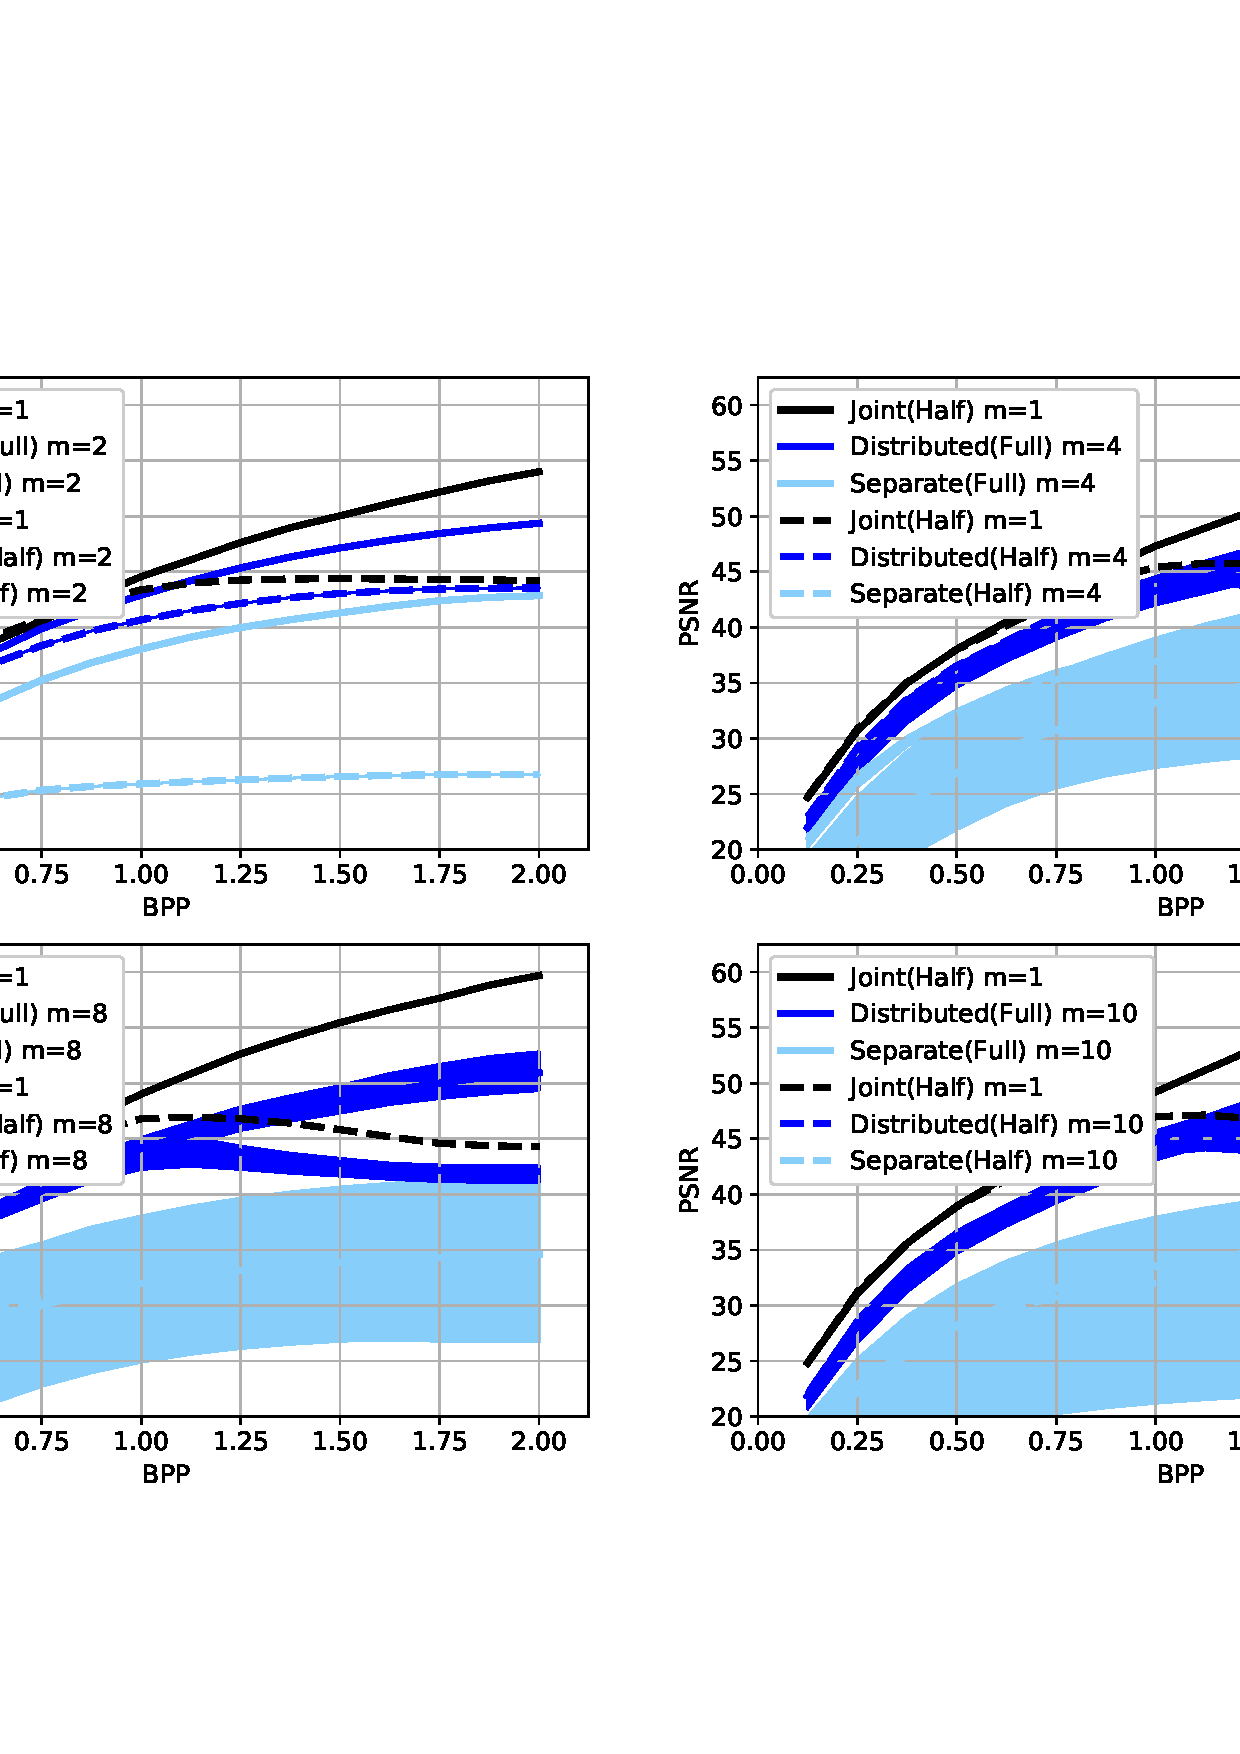
\includegraphics[width=0.8\linewidth]{half_class_band.png}
\end{center}
	\vspace{-0.2cm}
   \caption{Rate-distortion curves for data sources distributed by class labels with $T=16$ for the first half of sources and $T=8$ for the second half of sources.}
   \vspace{-0.2cm}
\label{fig_7}
\end{figure*}

\subsection{Arbitrary Correlated Sources}
To address the advantage of our DNN-based DSC framework, we first experiment distributed sources with different correlations. The distributed encoders are indexed as $1, \ldots, m$. We split data into random subsets and also split them by class labels. We show the result of data sources distributed by random subsets in Fig.~\ref{fig_4}, \ref{fig_6} and by class labels in Fig.~\ref{fig_5}, \ref{fig_7}. In the first case, each distributed encoder is trained with a subset of data and only the decoder can access the codes compressed from each data source. In the second case, we distribute data sources by class labels. For example, the $m$th encoder can only access data of digit $m-1$ and the label is $m-1$ ($m\leq 10$). %The theoretical limit in the case of $m<10$ is also obtained with data of digits with labels $<m$.

The curve of distributed encoders shows that the performance of training distributed encoders and joint decoder can be very close to the theoretical limit. As the number of encoders grows, the performance decreases a little, but still dominantly outperforms training codecs for each data source separately. From various experiments we found that the gap will become smaller when more data are available. The gap also diverges as more bits are generated. This is because the residual differences used as input at each iteration are less correlated among data sources than the original images. This experiment clearly shows that near-oracle performance can be achieved without specifically estimating the correlations among different sources, a desirable feature not enjoyed by classical DSC code design. The results show that our Deep DSC framework is able to adaptively learn arbitrary correlations among arbitrary number of data sources. 

\subsection{Low Complexity Encoding}
We also demonstrate the performance of low complexity encoders which are trained with less number of iterations. In this experiment, the first half of encoders are trained with $16$ iterations, labeled as \textit{Full}, and the second half of encoders are only trained with $8$ iterations, labeled as \textit{Half}. For example, for $m=8$, encoders $1$ to $4$ are trained with 16 iterations while encoders $5$ to $8$ are trained with 8 iterations. In Fig.~\ref{fig_6} and Fig.~\ref{fig_7}, we show the dashed lines for $T=8$ and solid lines for $T=16$ respectively. The theoretical limits (in black lines) are trained with all available data. The first half of encoders and the second half of encoders only access half of the whole dataset respectively.

Although the theoretical limits are obtained from all data, full and half complexity encoders %, only using half of the whole dataset, 
can still approach their theoretical limits (in black dash). Half complexity encoders perform as well as full complexity encoders in the first 8 iterations, because their correlations of the first eight iterations are trained properly with the model parameters. After the eighth iteration, both full and half complexity encoders can still approach their theoretical limits, because the trained correlations of residual differences from the first eight iterations can be reused at the second eight iterations without training. However, without specifically training the correlations after the eighth iterations, the performance of half complexity encoders slightly decreases when BPP is larger than 1. %a little compared to Fig.~\ref{fig_4} and \ref{fig_5}.


\subsection{Robust Distributed Encoding}
Our data-driven DSC framework, unlike classical DSC code design, does not require synchronization of data sources. In classical DSC code design, if syndrome bits $H(X|Y)$ are used and the data source $X$ is accidentally blocked, we will not be able to decode data source $Y$. As mentioned previously, we test each encoder separately with all test data once training is finished. Even only one of distributed encoders is functional, it can still benefits from its correlations with other sources because their correlations are already trained with the model parameters. 

%Our results are summarized 
%A confidence band is determined by the best and worst performance of all encoders at each iteration.
All our experiments show that distributed encoders not only dominates separately trained codecs but also have narrower confidence band. As the number of encoders increases, the confidence band of separately trained codecs becomes wider because each separate codec can only access very limited amount of data and thus suffer from overfitting. As the number of iterations increases, the confidence band also becomes wider. This is because the residual differences at later iterations become less correlated. Finally, the confidence band of data sources distributed by class labels is also wider than that of data sources distributed by random subsets. This is mainly because encoders specialize on data with the same label so their performance fluctuates more than encoders trained by data sources distributed by random subsets. %; 2 part of data sources distributed by class labels when $m<10$.
%------------------------------------------------------------------------
\section{Conclusion}
We introduce a data-driven Distributed Source Coding framework based on Deep Recurrent models. Compared to classical code design, our method has the following advantages. First, the compression quality of our recurrent model is scalable. Data sources can be efficiently compressed at different bit rates with a single recurrent model. Second, instead of explicitly estimating the correlations among data sources in advance, we use data-driven approach to learn the correlations with the neural network parameters. Therefore, given enough training data, our method can handle arbitrary number of sources with arbitrary correlations. Third, as one of the most important applications of Distributed Source Coding, low complexity encoder is also shown to be feasible based on our experimental results. Data sources trained with less data and fewer number of iterations can still approach the theoretical limit obtained when all data are used. Finally, we show the robustness of our framework. Unlike classical code design which may require careful data source synchronization, each distributed encoder of our model, once trained and deployed, can be used independently of others because the correlations are already learned by the model parameters. 

We point out two interesting directions of future work. First, training of the current architecture may be improved by introducing adaptive weights over different iterations, e.g. by using an attention mechanism. Second, the network architecture may be further extended to handle time-dependent data sources.
%We hope this work can pave a new way of practical distributed source code design.
\section*{Acknowledgement}
This work is supported by Office of Naval Research (ONR) grant numbers N00014-18-1-2244.
%------------------------------------------------------------------------
{%\small
\balance
\bibliographystyle{IEEEtran}
\documentclass[10pt,twocolumn,letterpaper]{article}

\usepackage{iccv}
\usepackage{times}
\usepackage{epsfig}
\usepackage{graphicx}
\usepackage{amsmath}
\usepackage{amssymb}
\usepackage{algorithm}
\usepackage{algorithmic}
\usepackage{balance}

% Include other packages here, before hyperref.
\usepackage{bm}

% If you comment hyperref and then uncomment it, you should delete
% egpaper.aux before re-running latex.  (Or just hit 'q' on the first latex
% run, let it finish, and you should be clear).
\usepackage[pagebackref=true,breaklinks=true,letterpaper=true,colorlinks,bookmarks=false]{hyperref}

\iccvfinalcopy % *** Uncomment this line for the final submission

\def\iccvPaperID{4386} % *** Enter the ICCV Paper ID here
\def\httilde{\mbox{\tt\raisebox{-.5ex}{\symbol{126}}}}

% Pages are numbered in submission mode, and unnumbered in camera-ready
\ificcvfinal\pagestyle{empty}\fi
\begin{document}

%%%%%%%%% TITLE
\title{Distributed Lossy Image Compression with Recurrent Networks}

\author{Enmao Diao\\
Duke University\\
{\tt\small enmao.diao@duke.edu}
% For a paper whose authors are all at the same institution,
% omit the following lines up until the closing ``}''.
% Additional authors and addresses can be added with ``\and'',
% just like the second author.
% To save space, use either the email address or home page, not both
\and
Jie Ding\\
University of Minnesota\\
{\tt\small dingj@umn.edu}
\and
Vahid Tarokh\\
Duke University\\
{\tt\small vahid.tarokh@duke.edu}
}

\maketitle
%\thispagestyle{empty}


%%%%%%%%% ABSTRACT
\begin{abstract}
We propose a new architecture for distributed image compression from a group of distributed data sources. The proposed architecture, which we refer to as symmetric Encoder-Decoder Convolutional Recurrent Neural Network, is able to significantly outperform the state-of-the-art compression techniques such as JPEG on rate-distortion curves. We also show that by training distributed encoders and joint decoders on correlated data sources, the performance of compression is much better than that by training codecs separately. For $10$ distributed sources, our distributed system remarkably performs within 2 dB peak signal-to-noise ratio (PSNR) of that of a single codec trained with all data sources. We experiment distributed sources with different correlations and show how our methodology well matches the Slepian-Wolf Theorem in Distributed Source Coding (DSC). Our method is also shown to be robust to the lack of presence of encoded data from a number of distributed sources. To the best of our knowledge, this is the first data-driven DSC framework for general distributed code design with Deep Learning.

\end{abstract}

%%%%%%%%% BODY TEXT
\section{Introduction}
It has been shown by a variety of previous works that Deep Neural Networks (DNN) can achieve comparable results as classical image compression techniques \cite{toderici2015variable,balle2016end,gregor2016towards,toderici2017full,theis2017lossy,johnston2017improved,liu2018cnn}. Most of these methods are based on autoencoder networks and quantization of bottleneck representations, e.g. by quantizing the codes into 8 bit integers and minimizing $\mathcal{L}_1$-penalized loss to sparsify the codes. These models usually rely on entropy codec to compress the sparsified codes. Moreover, to achieve different compression rates, it is unavoidable to train multiple models with different regularization parameters separately.

Among the existing literature of image compression, the recurrent neural network (RNN) based architecture \cite{toderici2015variable} is known to be the pioneering architecture that outperforms classical codecs. The model uses a recurrent autoencoder to encodes the residual difference between the original input and the reconstruction output. At each iteration, new binary coded information is extracted from the residual and the context from previous iterations is stored in the hidden state of the recurrent model. The compression rate, in this case, is varying according to the number of iterations of a single recurrent model. An improved architecture was proposed in \cite{johnston2017improved} that can simultaneously archive spatially adaptive bit rates in a single training phase. 

Motivated by various issues such as data privacy, computational cost, robustness against missing data, the following question has recently gained a lot of research interest. 

\textit{Can distributed encoders perform as well as a single encoder trained with all data sources together?} 

A positive answer from theoretical perspective was given in the context of Distributed Source Coding (DSC). 
In information theory, DSC is an important problem regarding the compression of multiple correlated data sources. The Slepian-Wolf Theorem shows that lossless coding of two or more correlated data sources with separate encoders and a joint decoder can compress data as efficiently as the optimal coding using a joint encoder and decoder \cite{slepian1973noiseless,cover1975proof}. The extension to lossy compression with Gaussian data sources was proposed as Wyner-Ziv Theorem \cite{wyner1976rate}. Although these theorems were published in 1970s, it was after about 30 years that practical applications such as Distributed Source Coding Using Syndromes (DISCUS) emerged \cite{pradhan2003distributed}. One of the main advantages of DSC is that the computation complexity of the encoder is shifted to the decoder. Typically, low complexity encoders can be used in multi-view video coding and sensor networks \cite{girod2005distributed,xiong2004distributed}. 
Motivated by the theoretical development of DSC, in this work we propose a DNN architecture that consists of distributed encoders and a joint decoder. We show that distributed encoders can perform as well as a single encoder trained with all data sources together.
Our proposed DSC framework is data-driven by nature, and it can be applied to distributed data even with unknown correlation structure.

\begin{figure}
\begin{center}
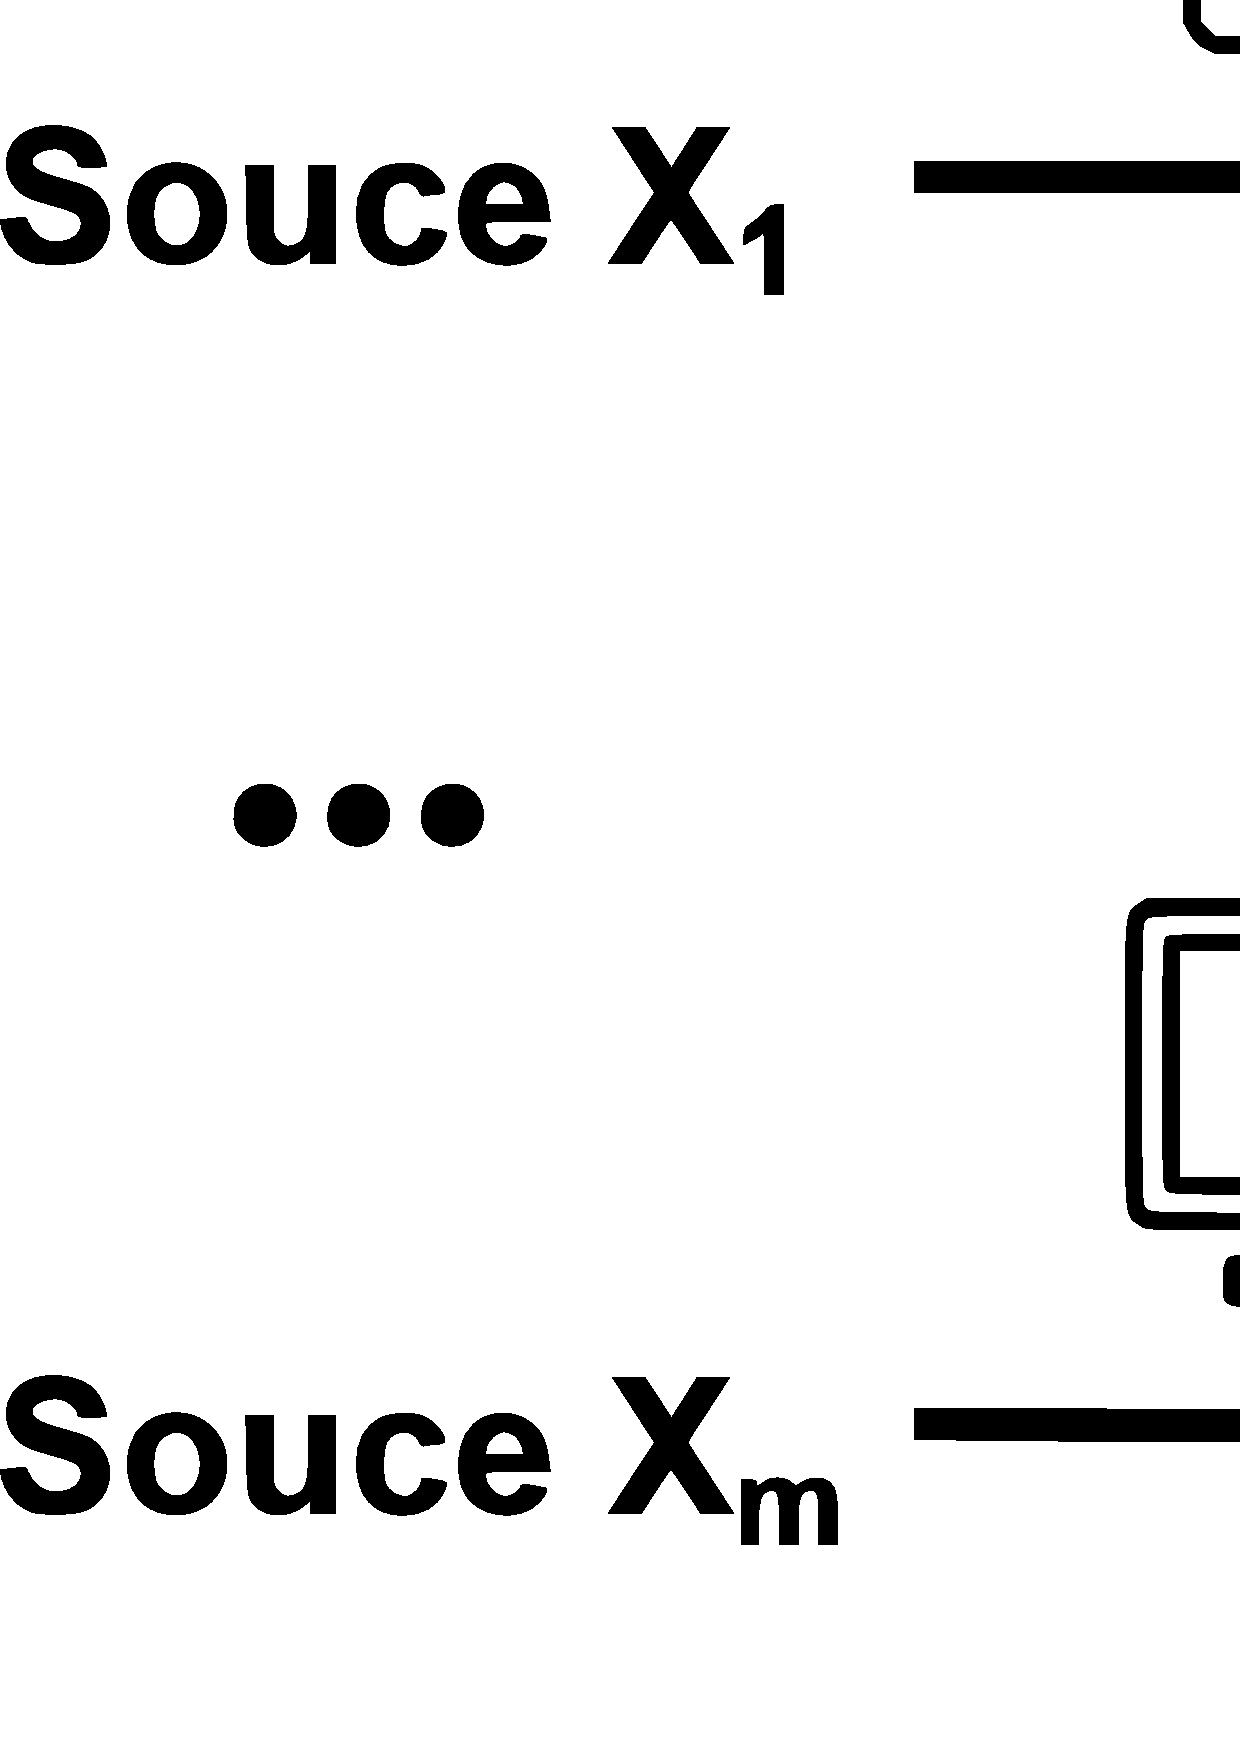
\includegraphics[width=1\linewidth]{DeepDSC.pdf}
\end{center}
   \caption{Illustration of Deep Distributed Source Coding.}
\label{fig_0}
\end{figure}

\begin{figure*}
\begin{center}
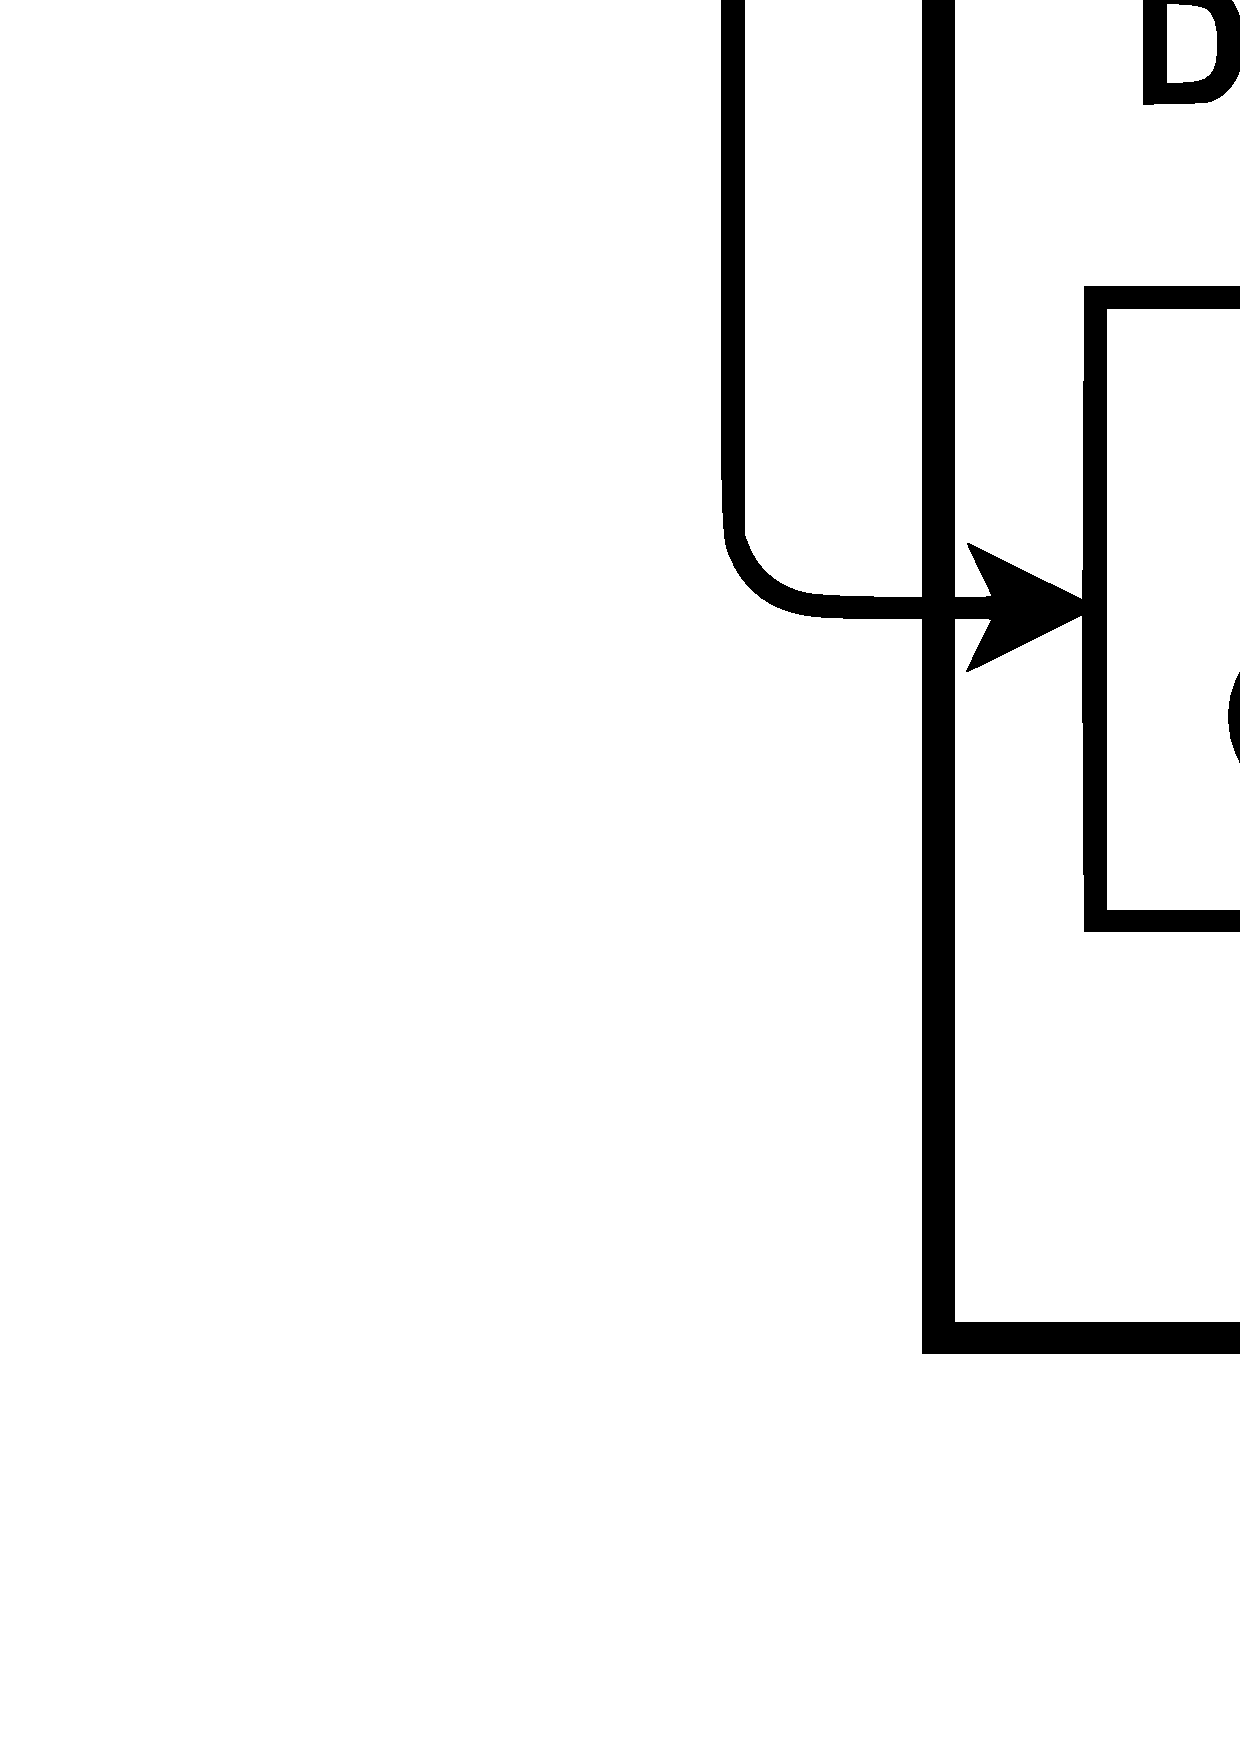
\includegraphics[width=0.8\linewidth]{DeepEncoderDecoder.pdf}
\end{center}
   \caption{Illustration of pixel-shuffled symmetric Encoder-Decoder architecture.}
\label{fig_1}
\end{figure*}
The advantages of our proposed architecture (illustrated in Fig.~\ref{fig_0} and \ref{fig_1}) are fourfold. 
First, the architecture is naturally scalable in the sense that codes can be decoded at more than one compression quality levels, and it allows efficient coding of correlated sources which are not physically co-located. This is especially attractive in video streaming applications \cite{guillemot2007distributed,gehrig2008distributed}. Second, unlike classical DSC which requires customized code design for different scenarios \cite{xiong2004distributed}, data-driven DSC framework can handle nontrivial distribution of image sources with arbitrary correlations. Third, the computation complexity of the encoder can be transferred to the decoder, a system of low complexity encoders can be used in a variety of application domains, such as multi-view video coding \cite{girod2005distributed}, sensor networks \cite{xiong2004distributed}, and under-water image processing where communication bandwidth and computational power are quite restricted \cite{stojanovic2009underwater,schettini2010underwater}. Fourth, the distributed framework can be more robust against heterogeneous noises or malfunctions of encoders, and such robustness can be crucial in, e.g., unreliable sensor networks \cite{girod2005distributed,ishwar2005rate,xiao2006distributed}.

The paper is outlined below. We review previous related work in Section 2 and describe our proposed method in details in Section 3. We describe our architecture for general image compression and its base modules in Section 3.1-3.4. Then we elaborate the Deep Distributed Source Coding framework in Section 3.5. Experimental results are shown in Section 4, followed by conclusions in Section 5.

%------------------------------------------------------------------------
\section{Related Work}
Though there has been a variety of research on lossy data compression in the past few decades, little attention has been paid to a systematic approach for general and practical distributed code design, especially in the presence of an arbitrary number of nontrivial data sources with arbitrary correlation %and possibly sources and correlation with memory. 
\cite{xiong2004distributed}. 
A main motivation of this work is to attempt to replace the practical hand-crafted code design with data-driven approaches. 
To our best knowledge, what we propose is the first data-driven DSC architecture. 
Unlike hand-crafted quantizers, our neural network-based quantizers show that the correlations among different data sources can be trained by the model parameters. We empirically show that the Slepian-Wolf limit can be achieved with our methodology. 

\subsection{Image compression with Deep Learning}
There exist a variety of classical codecs for lossy image compression. Although the JPEG standard \cite{wallace1992jpeg} was developed thirty years ago, it is still the most widely used image compression method. Several extensions to JPEG including JPEG2000 \cite{skodras2001jpeg}, WebP \cite{google2010webp} and BPG \cite{bellard2014bpg} have been developed. Most of these classical codecs rely on a quantization matrix applied to the coefficients of discrete cosine transform or wavelet transform.

The standard methods of compression with deep learning roughly fall into two categories. Non-recurrent autoencoders which rely on $\mathcal{L}_1$ penalty to sparsify the 8-bit integer codes, and recurrent models which introduce binary codes at each iteration. 
%Autoencoders are widely used as a general framework for neural network-based image compression. Bottleneck representations are quantized into 8-bit integers or binaries. 
The compression rate of non-recurrent models is not scalable and their performance heavily rely on the sparsity which entropy codec can take advantage of. 
Another challenge is to well define the derivative of quantizations of bottleneck representations. Ball\'e et al. \cite{balle2016end} replaced non-differentiable quantization step with a continuous relaxation by adding uniform noises. Toderici \cite{toderici2015variable}, on the other hand, used a stochastic form of binarization. 
The recurrent model~\cite{toderici2015variable,johnston2017improved}, on the other hand, has scalable compression rates. It generates more codes when the residual difference between the input and output of the model is compressed again.

\subsection{Distributed Source Coding}

\begin{figure}[t]
\begin{center}
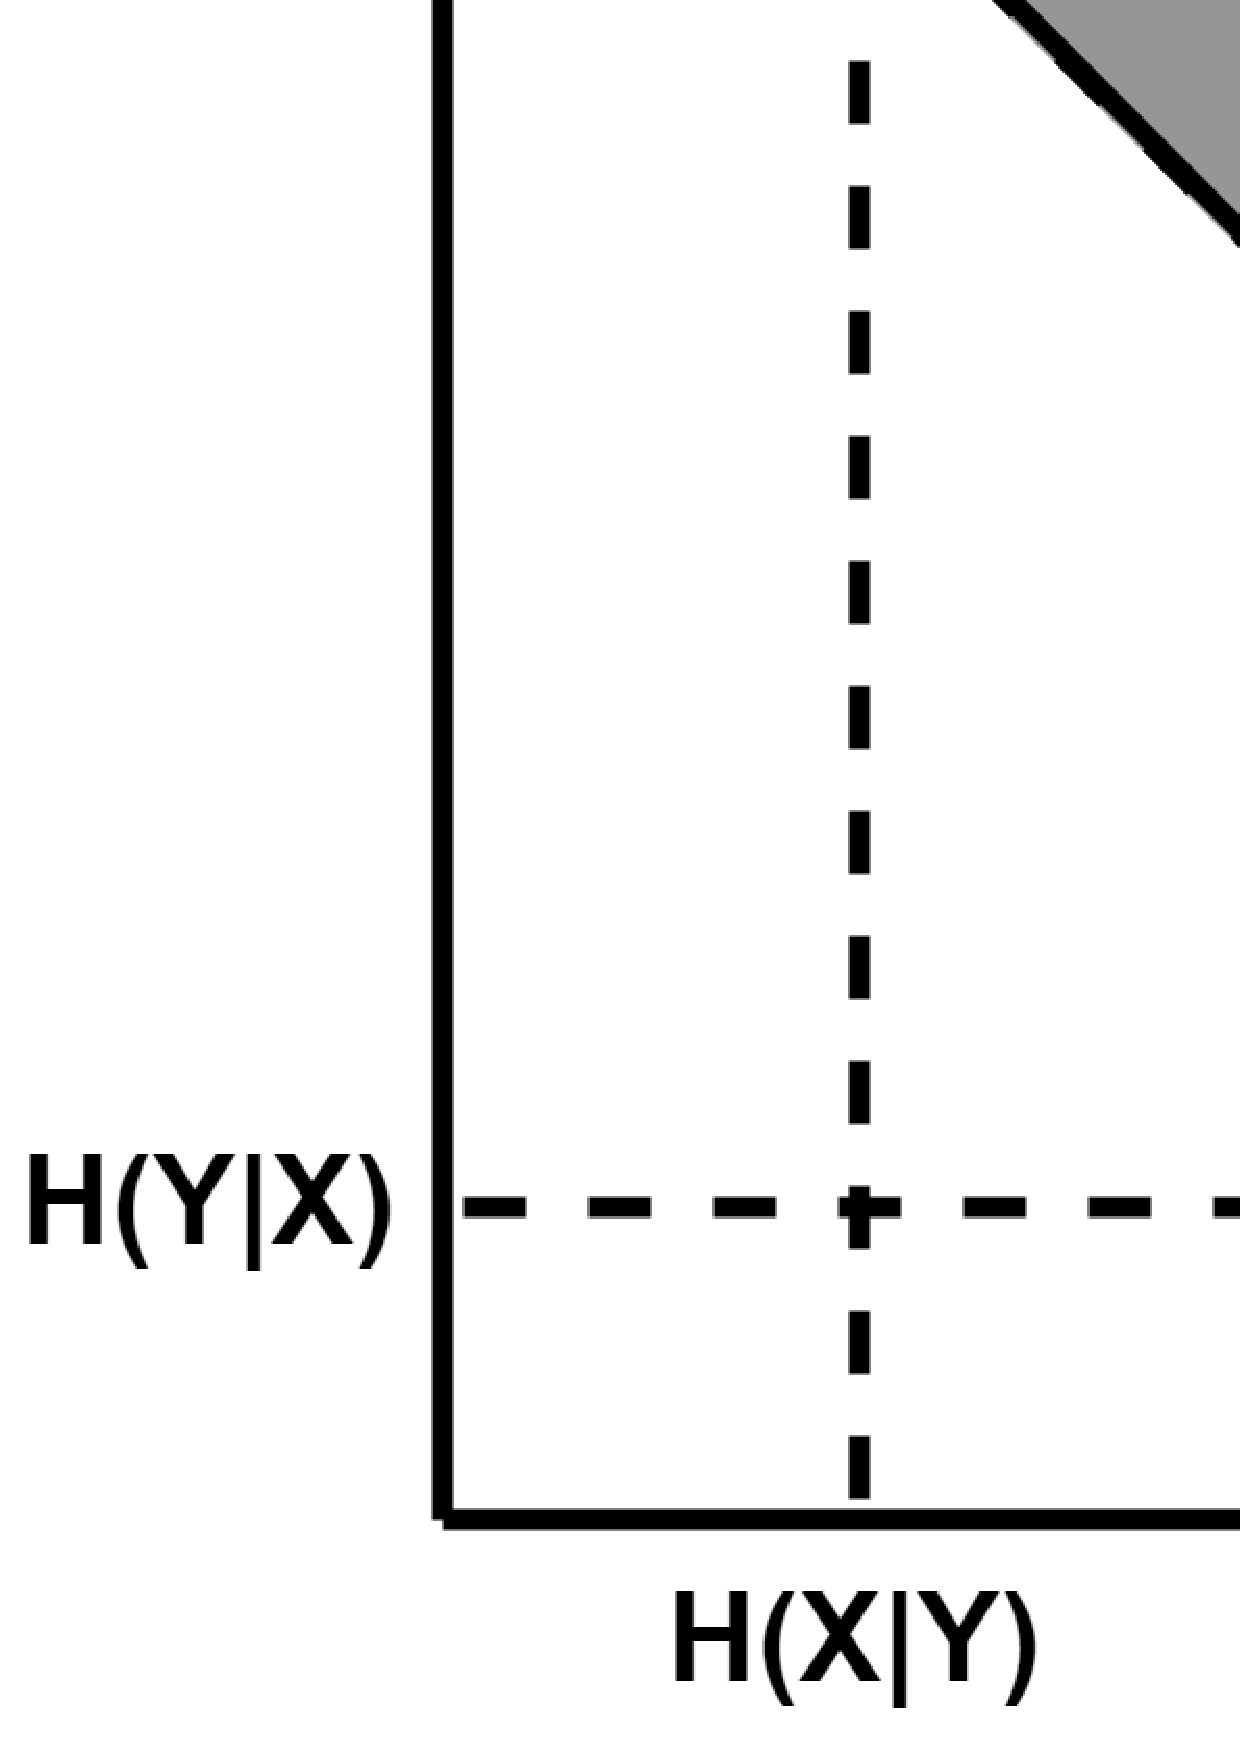
\includegraphics[width=0.8\linewidth]{SlepianWolf.pdf}
\end{center}
   \caption{The Slepian-Wolf achievable region for two sources $X$ and $Y$.}
\label{fig_2}
\end{figure}
Our methodology is deeply rooted in information-theoretic results on DSC which have been established since 1970s. The Slepian-Wolf \cite{slepian1973noiseless} Theorem shows that two correlated data sources encoded separately and decoded jointly can perform as well as joint encoding and decoding, and outperform separate encoding and separate decoding. The striking result indicates that as long as the codes are jointly decoded, there can be no loss in coding efficiency even the codes are separately encoded. Cover \cite{cover1975proof} generalizes the achievability of Slepian-Wolf coding to arbitrary number of correlated sources. Wyner-Ziv Coding \cite{wyner1976rate} gives a rate-distortion curve as an extension to lossy cases.

A classical illustration of Slepian-Wolf achievable region is shown in Fig.~\ref{fig_2}. We can achieve the performance of joint encoding and decoding of two data sources $X$ and $Y$ where the bit rate $R$ is equal to the joint entropy $H(X,Y)$ with separate encoding and joint decoding. Specifically, the achievable region proved by the Slepian-Wolf Theorem is given by $R_X\geq H(X|Y),R_Y\geq H(Y|X),$ and $R_X+R_Y\geq H(X,Y)$ as shown in the shaded area of Fig.~\ref{fig_2}. Here $R_{\cdot},H(\cdot)$ denote the bit rates and (conditional) entropies in classical Shannon theory. In practice, although some works are proposed to approach the mid-point $C$ \cite{schonberg2004distributed}, the most widely used scheme is source coding with side information (syndrome bits) at the decoder \cite{pradhan2003distributed}. This code design takes advantage of the corner points $A$ and $B$ which correspond to $R(X,Y) = R(Y)+R(X|Y)$ and $R(X,Y) = R(X)+R(Y|X)$ respectively. As an example, two 8-bit grayscale images $X$ and $Y$ have pixel values at the same location with (nonlinear) correlation implicitly determined by $x \in \{y-4, y-3, y-2, y-1, y, y+1, y+2, y+3\}$. Instead of sending 16 bits, we can send bits with $R=H(Y)+H(X|Y)$. We can take modulo of $x-y$ with respect to $8$ which only requires a 3-bit codebook $\tilde{x} \in \{4, 5, 6, 7, 0, 1, 2, 3\}$. Specifically, for $x=124$ and $y=128$, we transmit $\tilde{x}=(x-y) \mod 8$ which is 4 and $y=128$. The joint decoder will decode $x$ based on $y$ as $x = y-4 = 124$.

Some researchers have also shown the applicability of DSC on still images \cite{dikici2005distributed}. In practical applications, low complexity video encoding benefits from the DSC framework which can transfer the complexity of encoder to decoder \cite{puri2002prism,aaron2002wyner}. Scalable Video Coding can also be incorporated with DSC \cite{xu2006layered}. These proposed methods indicate the feasibility of DSC in our problem setting.

%-------------------------------------------------------------------------
\section{Methods}
In this section, we first describe the symmetric Encoder-Decoder architecture used in our research work. We will elaborate the base modules including Convolutional Long short-term memory (ConvLSTM), Pixel (Un)Shuffle, and Binarizer used in our model. We will then describe how this Deep Learning architecture is used in Distributed Source Coding framework.

\subsection{Network Architecture}
Our compression network consists of an encoder, a binarizer, and a decoder. The activation function following each Convolutional Neural Network (CNN) module is $\tanh$. For the first iteration of our model, the input images are initially encoded and transformed into $(-1,1)$ by $\tanh$ activation function. Binary codes are quantized from transformed bottleneck representations. The decoder then reconstructs images based on the received binary codes. Finally, we compute the residual difference between the original input images and the reconstructed output images. At the next iteration, the residual difference is feedback as the new input for our model. This procedure is repeated multiple iterations to gain more codes for better reconstruction performance. Therefore, the reconstructed images at each iteration are the sum of output reconstructions from previous and current iterations.

Consider dataset $X = \{x\}^{N}$ consisting of $N$ i.i.d. samples of some continuous or discrete variables $x$. The data generating process is unknown. Autoencoders for compression and reconstruction can be formulated in the following way. Data can be compressed with a neural network-based encoder $f(x;\theta)$ into quantized codes $\tilde{z}$ and reconstructed with a decoder $g(\tilde{z};\phi)$. We can binarize bottleneck representations $z$ and control the compression quality by varying its channel sizes. The loss function $\mathcal{L}(x,\tilde{x})$ is minimized with respect to the model parameters $\theta$ and $\phi$.
\begin{align}
z &= f(x;\theta),\\
\tilde{z} &= \text{Binarize}(z),\\
\tilde{x} &= g(\tilde{z};\phi),\\
\text{Minimize } \mathcal{L}&(x,\tilde{x})
\end{align}
Deep recurrent autoencoder gradually increases compression quality by creating a correlated residual sequence from the difference between the input and output of our model. The advantage of recurrent model is that we can train one model with scalable compression quality. Classical autoencoders, on the contrary, have to train multiple networks with different penalty coefficients or channel sizes for different compression qualities. Suppose $T$ iterations are used, we can formulate the recurrent autoencoder in the following way.
\begin{align}
z_t &= f(x_t;\theta),\\
\tilde{z}_t &= \text{Binarize}(z_t),\\
\tilde{x}_t &= g(\tilde{z}_t;\phi),\\
x_{t+1} &= x_t-\tilde{x}_t\text{, }\tilde{x}_1=0,\\
\text{Minimize } \frac{1}{T}&\sum_{t=1}^{T}\mathcal{L}(x_1,\sum_{i=1}^{t}\tilde{x}_i).
\end{align}
In the recurrent autoencoder, the compression quality is controlled by several factors including the scale factor of Pixel (Un)Shuffle module $r$, the depth of model $D$, the channel size of bottleneck representations $C$, and the number of iterations $T$. The height and width of bottleneck representations are determined by $T$ and $D$. As we have $N$ batch images with shape $H,W$, the size of codes after $T$ iterations is $(N,T,C,H/(r^D),W/(r^D))$. For example, with $r=2$, $D=3$, and $C=2^D$, one $32 \times 32$ RGB image will generate $(1,1,8,4,4)$ binary codes for a single iteration. Thus, we will add up $\frac{8
\times4\times4}{32\times32} = 0.125$ Bit Per Pixel (BPP) for this iteration. Although we configure these hyper-parameters, we believe it is possible to train these configurations in future works.

\subsection{Convolutional Long short-term memory}
As proposed by \cite{xingjian2015convolutional}, simply replacing the Fully Connected (FC) layer in LSTM with convolutional layer, ConvLSTM is able to capture spatial structure in the temporal sequence. We do not add any bias term to our modules because the output of each layer is saturated by $\tanh$. The key equations are shown below.
\begin{align}
i_t &= \sigma(W_{xi}*x_t + W_{hi}*h_{t-1}) ,\\
f_t &= \sigma(W_{xf}*x_t + W_{hf}*h_{t-1}) ,\\
c_t &= f_tc_{t-1}+i_t\tanh(W_{xc}*x_t + W_{hc}*h_{t-1}), \\
o_t &= \sigma(W_{xo}*x_t + W_{ho}*h_{t-1}) ,\\
h_t &= o_t\tanh(c_t).
\end{align}
The first and last layers of the encoder and decoder are feed-forward Convolutional Neural Network with $\tanh$ activations. The recurrent layers are all ConvLSTM networks. We do not replace CNN layer with ConvLSTM because the size of the feature maps of hidden state at shallow layers cost a mass amount of memory. From our various experimental studies, the performance does not degrade significantly either because no convolutional layers are in between ConvLSTM layers.

\subsection{Pixel (Un)Shuffle}
We resize feature maps with Pixel (Un)Shuffle modules. Pixel Shuffle module is originally proposed by \cite{shi2016real} to tackle image and video super-resolution problem. Compared to bilinear interpolation and tranposed convolutional layers, Pixel Shuffle module is much more computationally efficient, because it is non-parametric and only requires tensor reshaping and dimension permutation. We note that although this method is widely used for upscaling, it is actually invertible and we propose to use its inversion for downscaling. Thus, the encoder and decoder can be constructed symmetrically. Our experimental results show that symmetric Encoder-Decoder architecture actually produces much better results with less number of parameters, compared to the asymmetric architecture as proposed in \cite{toderici2017full}. We describe these two modules with the following pseudocodes \ref{alg_0} and \ref{alg_1}.

\begin{algorithm}
\caption{Pixel UnShuffle}
\begin{algorithmic}
\label{alg_0}
\REQUIRE $X\sim(N,C,H,W)$, $r_H,r_W$
\ENSURE $r_H,r_W$ are integers, divides $H,W$
\STATE Reshape $X\sim(N,C,H/r_H,r_H,W/r_W,r_W)$
\STATE Permute $X\sim(N,C,r_H,r_W,H/r_H,W/r_W)$
\STATE Reshape $X\sim(N,C\times r_H\times r_W,H/r_H,W/r_W)$
\end{algorithmic}
\end{algorithm}

\begin{algorithm}
\caption{Pixel Shuffle}
\begin{algorithmic}
\label{alg_1}
\REQUIRE $X\sim(N,C,H,W)$, $r_H,r_W$
\ENSURE $r_H,r_W$ are integers, $r_H\times r_W$ divides $C$
\STATE Reshape $X\sim(N,C/(r_H \times r_W),r_H,r_W,H,W)$
\STATE Permute $X\sim(N,C/(r_H \times r_W),H,r_H,W,r_W)$
\STATE Reshape $X\sim(N,C/(r_H \times r_W),H \times r_H,W \times r_W)$
\end{algorithmic}
\end{algorithm}

\subsection{Binarizer}
The derivative of quantization function is only defined at the rounded integer itself. Therefore, we have to replace its derivative in the backward pass of backpropagation with a form of smooth approximation \cite{rumelhart1988learning}. Thanks to a thorough discussion of different alternative approaches by \cite{theis2017lossy}, we choose to use identity function to replace its derivatives that cannot be well defined as shown in \ref{eq_15}. During training, we use a stochastic form of binarization proposed by \cite{toderici2017full}. For bottleneck representations $z \in (-1,1)$, the details of binarizer $\tilde{z}=\text{Binarize}(z)$ are described as follows, where $W_{\cdot}$ denote the standard parameter matrices between two network layers.
\begin{align}
\intertext{\textbf{Train}}
\tilde{z}=\text{Binarize}(z) &= 
    \begin{cases}
      1, &  \text{with probability } (z+1)/2\\
      -1, & \text{otherwise}
      \end{cases} \nonumber \\
\frac{d}{dz}\tilde{z} &:= \frac{d}{dz}\mathbb{E} (\tilde{z}) =  \frac{d}{dz}\mathbb{E} (z) = 1\label{eq_15}
\intertext{\textbf{Test}}
\text{Binarize}(z) &= 
    \begin{cases}
      1, & \text{if } z\geq0 \\
      -1, & \text{otherwise}
      \end{cases}
\end{align}

\subsection{Deep Distributed Source Coding Framework}
Fig.~\ref{fig_0} and \ref{fig_1} illustrates our Deep DSC coding framework. Similar to classical DSC framework, each data source is encoded separately and decoded jointly. Traditionally, researchers have to design different kind of codes for specific scenarios \cite{schonberg2004distributed}. We propose to use data-driven approach to handle complex scenarios where the distribution of data sources are unknown and their correlations can be arbitrary. Our proposal may also shed new light on sophisticated application scenarios such as videos where data sources and correlations are time dependent.

In our neural network-based DSC, %the whole encoding and decoding procedure are trained jointly. 
$M$ distributed encoders encode corresponding data sources $x^m$ that can be arbitrarily correlated. Each neural network-based encoder $f(x^m;\theta^m)$ has their own model parameters $\theta^m$. After binarizing bottleneck representations $z^m$, code sources $\tilde{z}^m$ are transmitted and concatenated batch-wisely. A single decoder $g(\tilde{z}^m;\phi)$ reconstructs images $\tilde{x}^m$ from all sources with the same model parameters $\phi$. 
In particular, the parameters of the following model are optimized with backward propagation \cite{rumelhart1988learning}. 
\begin{align}
z_t^m &= f(x_t^m;\theta^m),\\
\tilde{z}_t^m &= \text{Binarize}(z_t^m),\\
\tilde{x}_t^{m} &= g(\tilde{z}_t^{m};\bm{\phi}),\\
x_{t+1}^{m} &= x_t^{m}-\tilde{x}_t^{m}\text{, }\tilde{x}_1^{m}=0,
\end{align}
\begin{align}
\text{Minimize } \frac{1}{MT}&\sum_{t=1}^{T}\sum_{m=1}^{M}\mathcal{L}(x_1^m,\sum_{i=1}^{t}\tilde{x}_i^m).
\end{align}
Our result shows that the resulting distributed model can perform as well as encoding all data by one single encoder. However, if we encode and decode each data source separately, the performance becomes significantly worse. Moreover, correlations among data sources cannot be learned with separate parameters of decoders, i.e. with 
$\tilde{x}_t^{m} = g(\tilde{z}_t^{m};\bm{\phi^m})$.
%------------------------------------------------------------------------
\section{Experiments}
We use MNIST dataset \cite{lecun1998gradient} consisting of 60,000 training and 10,000 testing grayscale handwritten digit images. The digits have been resized from $28 \times 28$ to $32 \times 32$. The Adam optimizer \cite{kingma2014adam} is used with $\epsilon = 1e-8$, $\beta_1 = 0.9$ and $\beta_2 = 0.999$. We train model with $\mathcal{L}_1$ loss, batch size $N=100$ and learning rate $0.001$ for a total of 200 epochs. We start to decay learning rate by half at the 70th epoch and at every 20 epochs thereafter.

As described in section 3.1, we set the scaling factor for Pixel (Un)Shuffle module to be $r=2$, depth of model $D=3$, and code channel size $C=2^D$. For $T=16$, one minibatch of grayscale images with shape $(100,1,32,32)$ will be encoded to be a $(100,16,8,4,4)$ binary tensor. We evaluate all models with the metric Peak Signal to Noise Ratio (PSNR) against the Bit Per Pixel (BPP).

\begin{figure}[t]
\begin{center}
\includegraphics[width=0.8\linewidth]{codec.pdf}
\end{center}
	\vspace{-0.2cm}
   \caption{Our symmetric pixel-shuffled Encoder-Decoder outperforms classical codecs and baseline neural network-based codecs.}
   \vspace{-0.2cm}
\label{fig_3}
\end{figure}

We compare our model to the baseline model \cite{toderici2017full} and classical codecs like JPEG~\cite{wallace1992jpeg}, JPEG2000~\cite{skodras2001jpeg} and BPG~\cite{bellard2014bpg}. To directly compare the performance of network architecture, we ignore some techniques introduced by \cite{toderici2017full} and \cite{johnston2017improved} such as progressive entropy coding and hidden-state priming. Instead of bilinear interpolation or convolutional layers used in previous works\cite{toderici2017full,theis2017lossy,johnston2017improved}, our network architecture uses Pixel Shuffle in the Encoder. As a result, our network architecture has a symmetric Encoder-Decoder structure and also few number of parameters. Fig.~\ref{fig_3} shows that our symmetric pixel-shuffled Encoder-Decoder architecture outperforms classical codecs and baseline neural network-based codecs.

We run experiments with $(2,4,8,10)$ number of distributed sources. Each encoder encodes data from each data source without communicating with other encoders. The decoder jointly decodes the codes gathered from each distributed encoder. First, we compare our result, labeled as \textit{Distributed}, to the case where all data are trained with one encoder and one decoder jointly, labeled as \textit{Joint}. The `Joint' curve is approximated as the theoretical upper bound of performance. %theoretical upper bound $H(X,Y)$. 
Second, we compare our result to the case where each data source is trained with a separate pair of encoder and decoder, labeled as \textit{Separate}. We test each distributed encoder separately with all test data. The solid curves are the average performance across all encoders. At each iteration, the confidence band is determined by the best and worst performance of all encoders. 

Our experimental studies in the following sections consist of three aspects. We first experiment data sources with different correlations. We then show the performance of low complexity encoders which are trained with less number of iterations. Finally, we show the robustness of our distributed framework in the absence of a number of distributed sources.

\begin{figure*}
\begin{center}
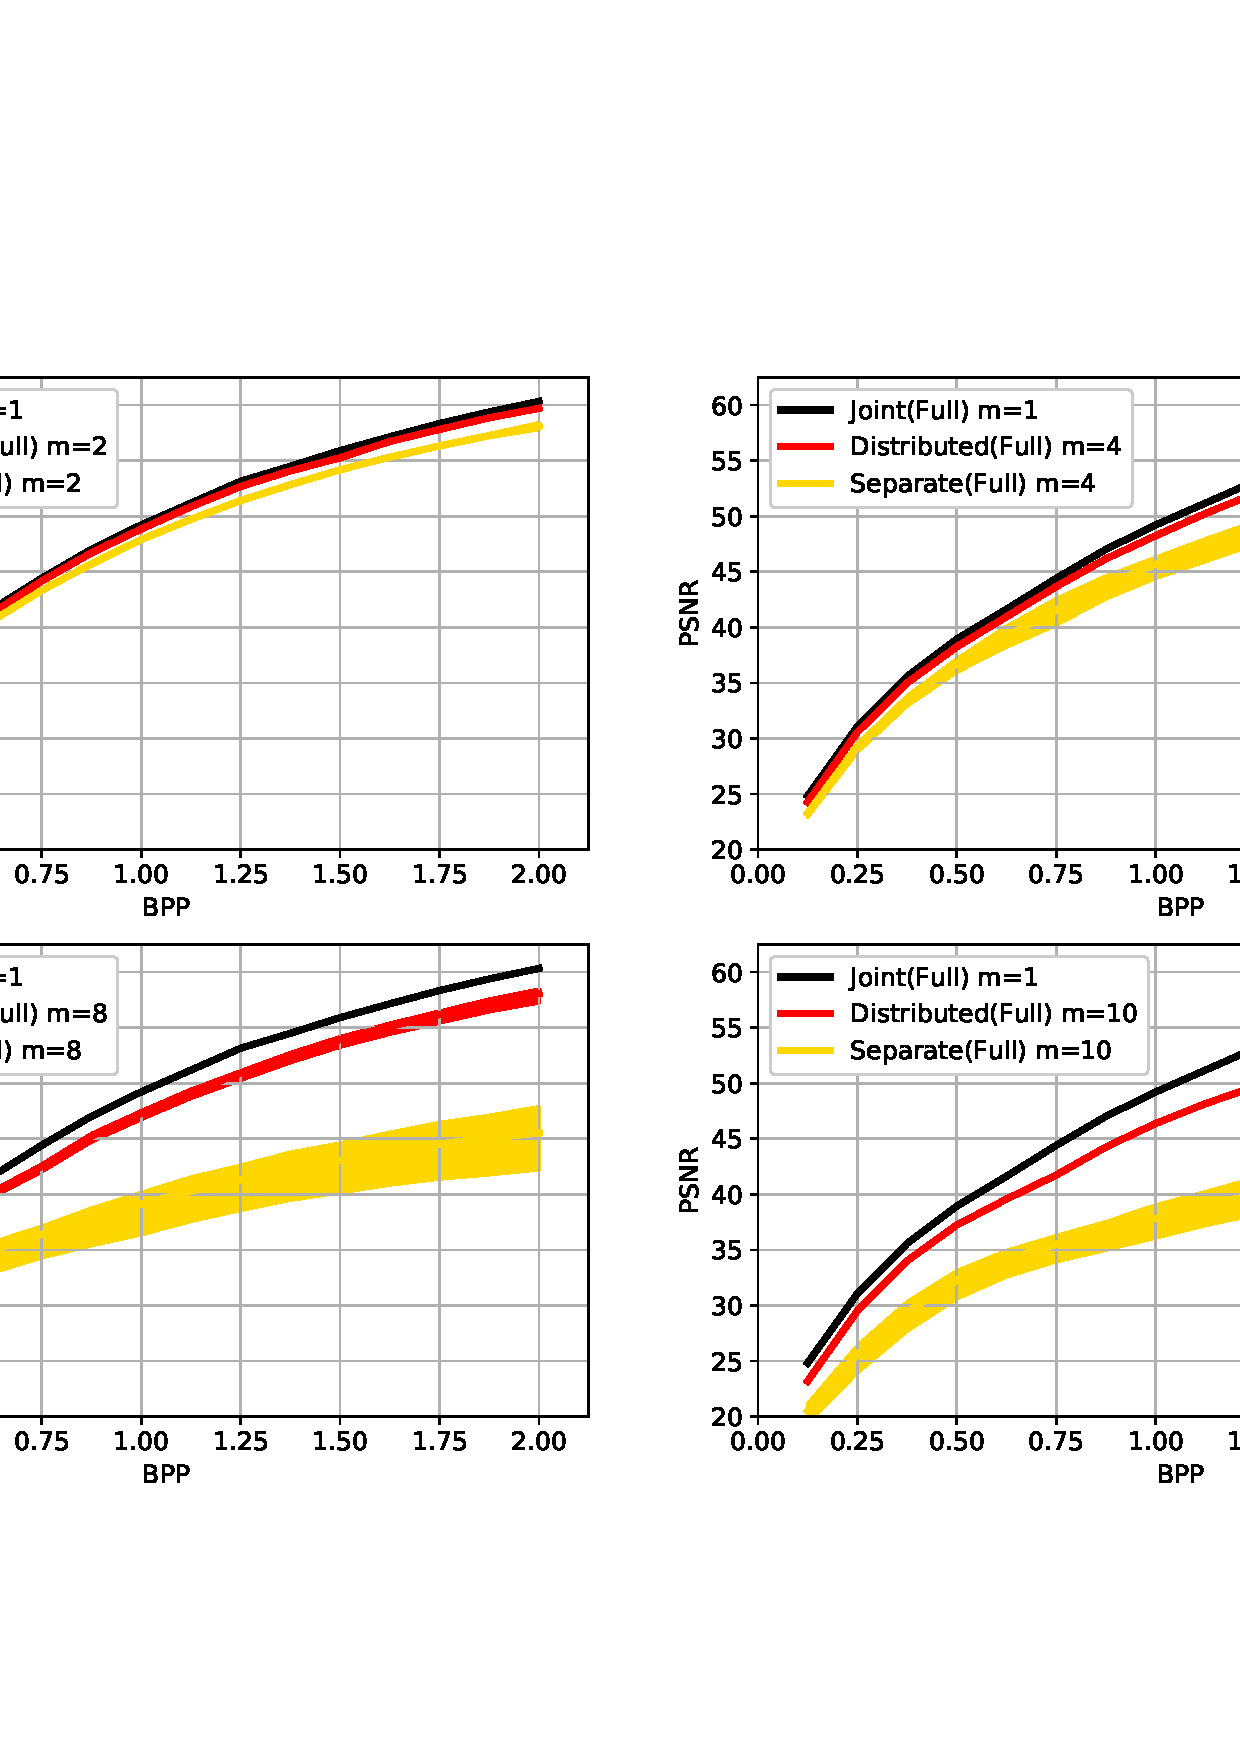
\includegraphics[width=0.8\linewidth]{full_subset_band.png}
\end{center}
	\vspace{-0.2cm}
   \caption{Rate-distortion curves for data sources distributed by random subsets with $T=16$ for all sources.}
   \vspace{-0.2cm}
\label{fig_4}
\end{figure*}

\begin{figure*}
\begin{center}
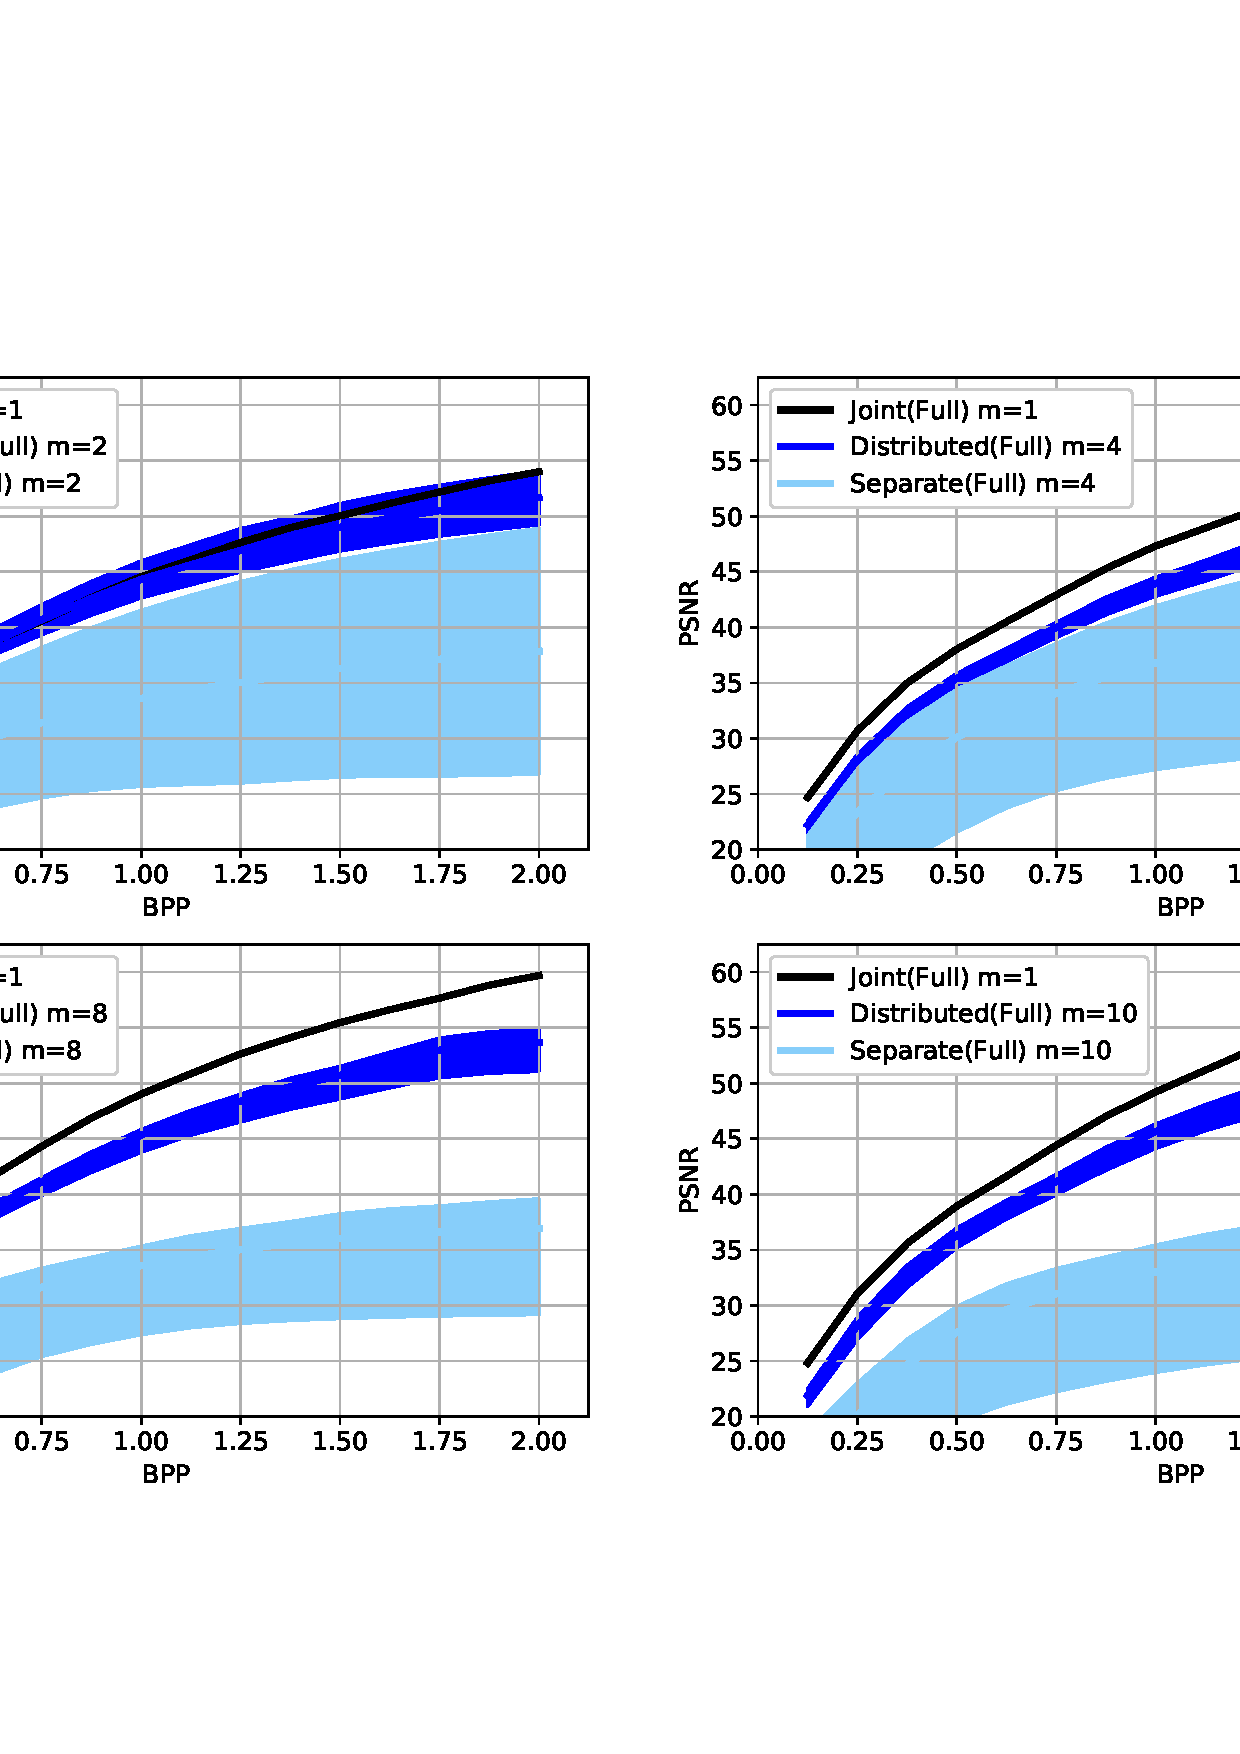
\includegraphics[width=0.8\linewidth]{full_class_band.png}
\end{center}
	\vspace{-0.2cm}
   \caption{Rate-distortion curves for data sources distributed by class labels with $T=16$ for all sources.}
   \vspace{-0.2cm}
\label{fig_5}
\end{figure*}

\begin{figure*}
\begin{center}
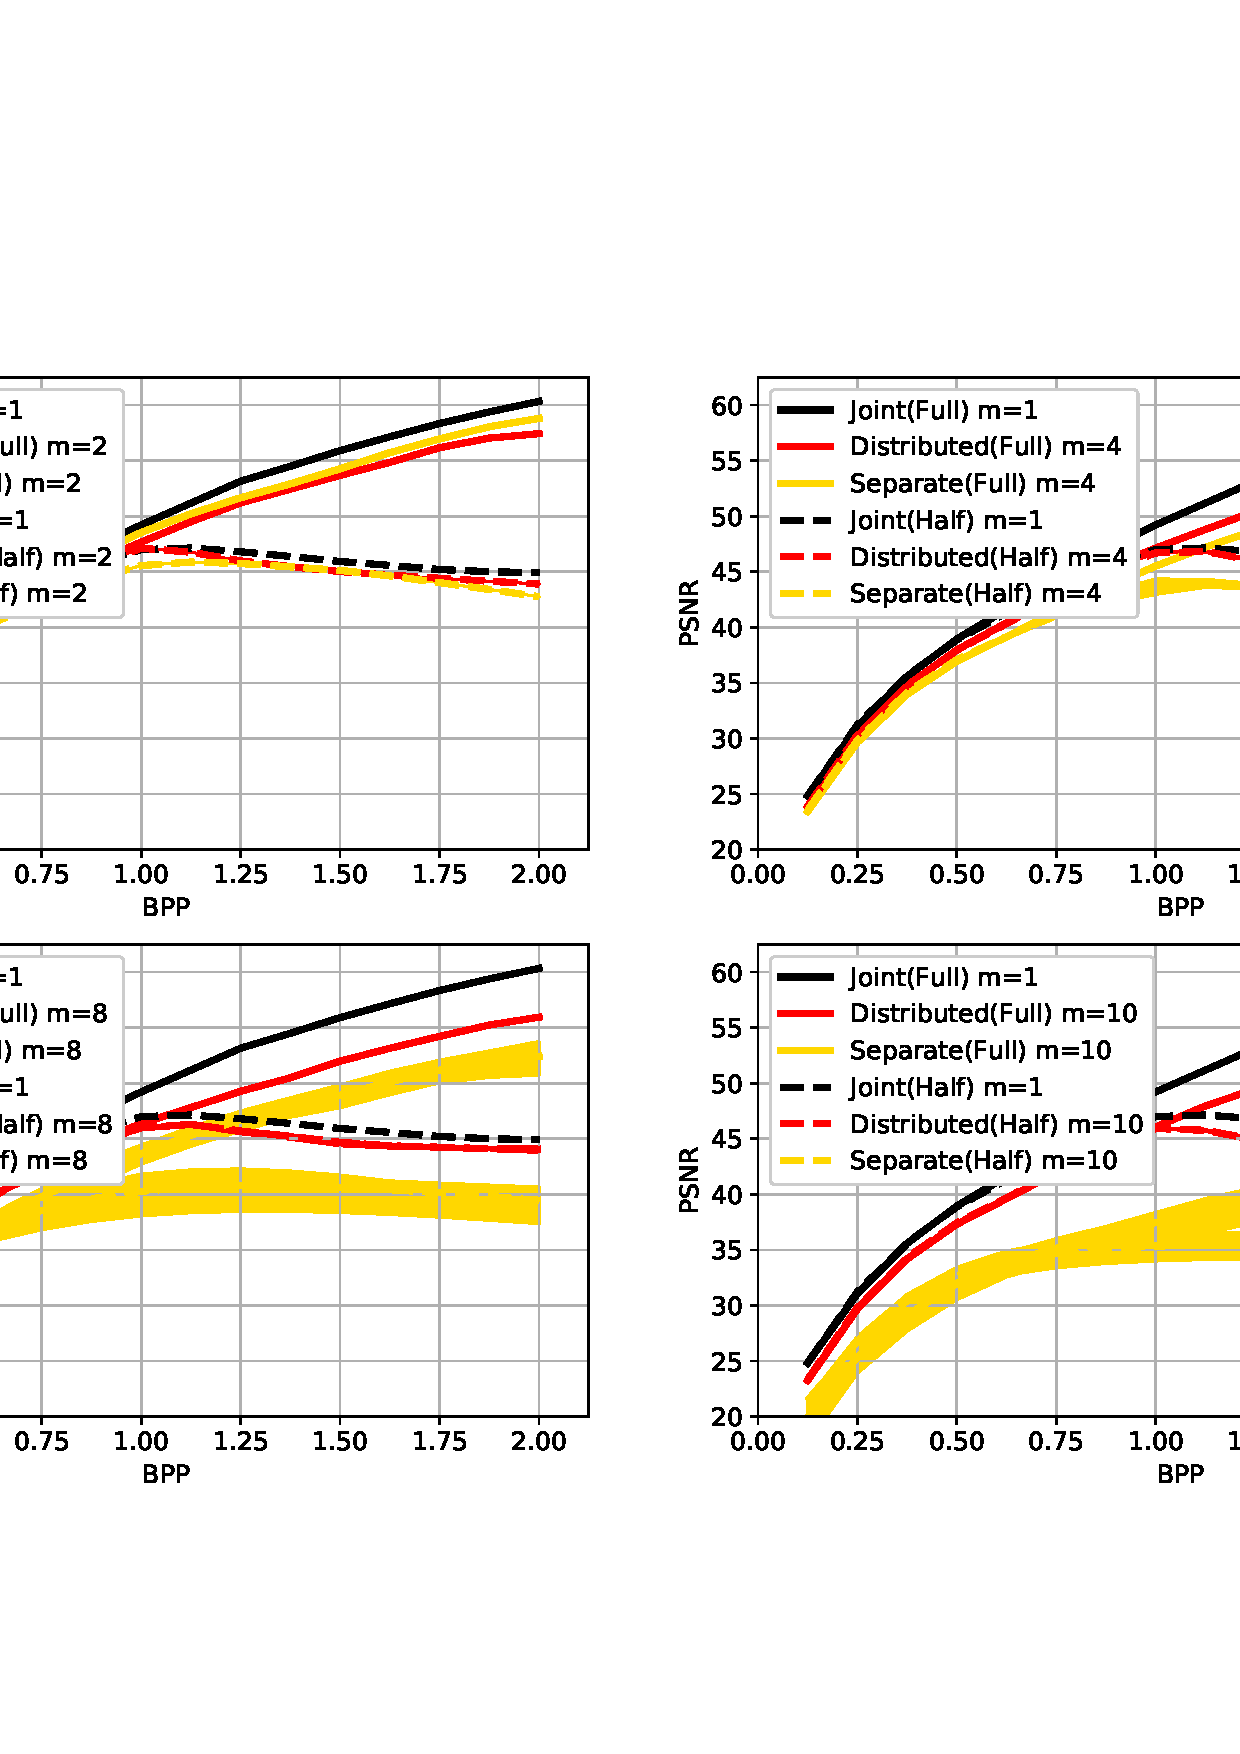
\includegraphics[width=0.8\linewidth]{half_subset_band.png}
\end{center}
	\vspace{-0.2cm}
   \caption{Rate-distortion curves for data sources distributed by random subsets with $T=16$ for the first half of sources and $T=8$ for the second half of sources.}
   \vspace{-0.2cm}
\label{fig_6}
\end{figure*}

\begin{figure*}
\begin{center}
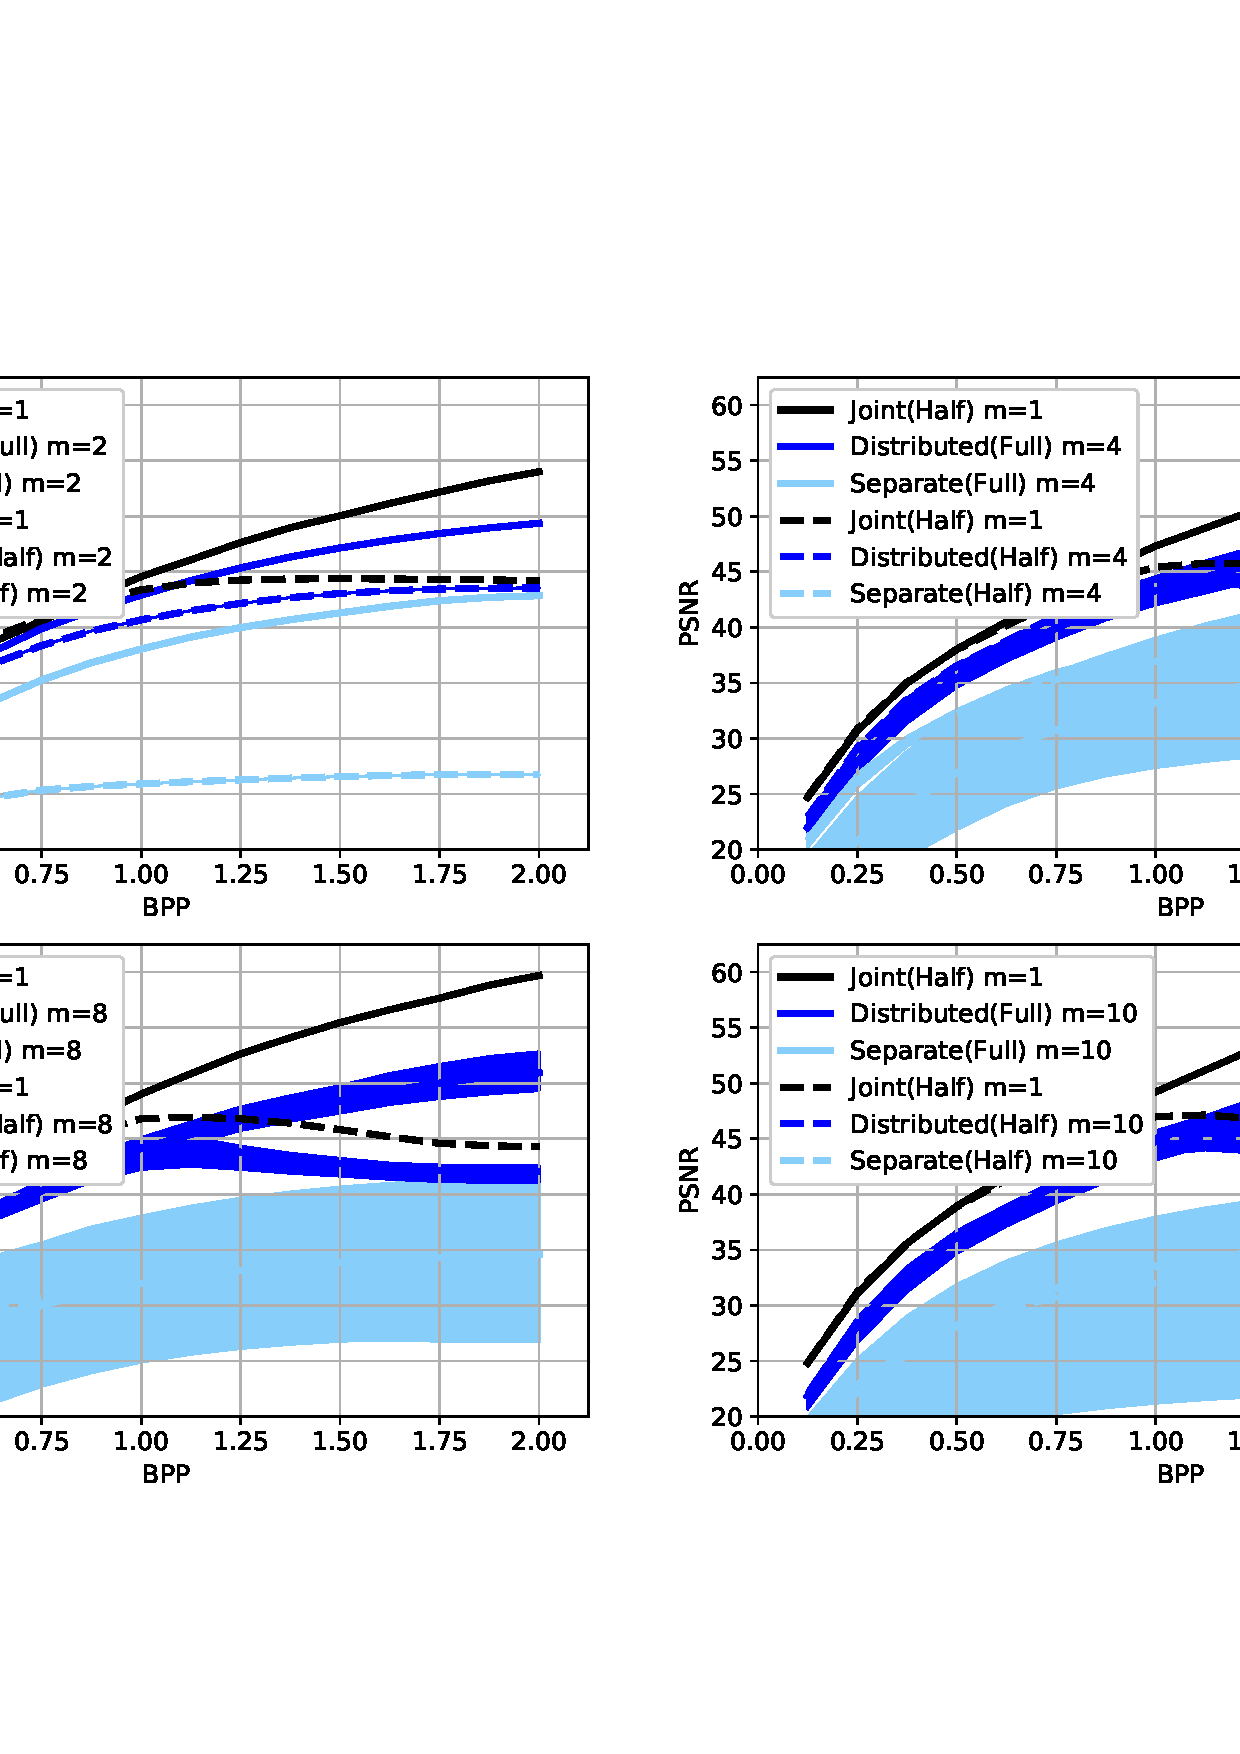
\includegraphics[width=0.8\linewidth]{half_class_band.png}
\end{center}
	\vspace{-0.2cm}
   \caption{Rate-distortion curves for data sources distributed by class labels with $T=16$ for the first half of sources and $T=8$ for the second half of sources.}
   \vspace{-0.2cm}
\label{fig_7}
\end{figure*}

\subsection{Arbitrary Correlated Sources}
To address the advantage of our DNN-based DSC framework, we first experiment distributed sources with different correlations. The distributed encoders are indexed as $1, \ldots, m$. We split data into random subsets and also split them by class labels. We show the result of data sources distributed by random subsets in Fig.~\ref{fig_4}, \ref{fig_6} and by class labels in Fig.~\ref{fig_5}, \ref{fig_7}. In the first case, each distributed encoder is trained with a subset of data and only the decoder can access the codes compressed from each data source. In the second case, we distribute data sources by class labels. For example, the $m$th encoder can only access data of digit $m-1$ and the label is $m-1$ ($m\leq 10$). %The theoretical limit in the case of $m<10$ is also obtained with data of digits with labels $<m$.

The curve of distributed encoders shows that the performance of training distributed encoders and joint decoder can be very close to the theoretical limit. As the number of encoders grows, the performance decreases a little, but still dominantly outperforms training codecs for each data source separately. From various experiments we found that the gap will become smaller when more data are available. The gap also diverges as more bits are generated. This is because the residual differences used as input at each iteration are less correlated among data sources than the original images. This experiment clearly shows that near-oracle performance can be achieved without specifically estimating the correlations among different sources, a desirable feature not enjoyed by classical DSC code design. The results show that our Deep DSC framework is able to adaptively learn arbitrary correlations among arbitrary number of data sources. 

\subsection{Low Complexity Encoding}
We also demonstrate the performance of low complexity encoders which are trained with less number of iterations. In this experiment, the first half of encoders are trained with $16$ iterations, labeled as \textit{Full}, and the second half of encoders are only trained with $8$ iterations, labeled as \textit{Half}. For example, for $m=8$, encoders $1$ to $4$ are trained with 16 iterations while encoders $5$ to $8$ are trained with 8 iterations. In Fig.~\ref{fig_6} and Fig.~\ref{fig_7}, we show the dashed lines for $T=8$ and solid lines for $T=16$ respectively. The theoretical limits (in black lines) are trained with all available data. The first half of encoders and the second half of encoders only access half of the whole dataset respectively.

Although the theoretical limits are obtained from all data, full and half complexity encoders %, only using half of the whole dataset, 
can still approach their theoretical limits (in black dash). Half complexity encoders perform as well as full complexity encoders in the first 8 iterations, because their correlations of the first eight iterations are trained properly with the model parameters. After the eighth iteration, both full and half complexity encoders can still approach their theoretical limits, because the trained correlations of residual differences from the first eight iterations can be reused at the second eight iterations without training. However, without specifically training the correlations after the eighth iterations, the performance of half complexity encoders slightly decreases when BPP is larger than 1. %a little compared to Fig.~\ref{fig_4} and \ref{fig_5}.


\subsection{Robust Distributed Encoding}
Our data-driven DSC framework, unlike classical DSC code design, does not require synchronization of data sources. In classical DSC code design, if syndrome bits $H(X|Y)$ are used and the data source $X$ is accidentally blocked, we will not be able to decode data source $Y$. As mentioned previously, we test each encoder separately with all test data once training is finished. Even only one of distributed encoders is functional, it can still benefits from its correlations with other sources because their correlations are already trained with the model parameters. 

%Our results are summarized 
%A confidence band is determined by the best and worst performance of all encoders at each iteration.
All our experiments show that distributed encoders not only dominates separately trained codecs but also have narrower confidence band. As the number of encoders increases, the confidence band of separately trained codecs becomes wider because each separate codec can only access very limited amount of data and thus suffer from overfitting. As the number of iterations increases, the confidence band also becomes wider. This is because the residual differences at later iterations become less correlated. Finally, the confidence band of data sources distributed by class labels is also wider than that of data sources distributed by random subsets. This is mainly because encoders specialize on data with the same label so their performance fluctuates more than encoders trained by data sources distributed by random subsets. %; 2 part of data sources distributed by class labels when $m<10$.
%------------------------------------------------------------------------
\section{Conclusion}
We introduce a data-driven Distributed Source Coding framework based on Deep Recurrent models. Compared to classical code design, our method has the following advantages. First, the compression quality of our recurrent model is scalable. Data sources can be efficiently compressed at different bit rates with a single recurrent model. Second, instead of explicitly estimating the correlations among data sources in advance, we use data-driven approach to learn the correlations with the neural network parameters. Therefore, given enough training data, our method can handle arbitrary number of sources with arbitrary correlations. Third, as one of the most important applications of Distributed Source Coding, low complexity encoder is also shown to be feasible based on our experimental results. Data sources trained with less data and fewer number of iterations can still approach the theoretical limit obtained when all data are used. Finally, we show the robustness of our framework. Unlike classical code design which may require careful data source synchronization, each distributed encoder of our model, once trained and deployed, can be used independently of others because the correlations are already learned by the model parameters. 

We point out two interesting directions of future work. First, training of the current architecture may be improved by introducing adaptive weights over different iterations, e.g. by using an attention mechanism. Second, the network architecture may be further extended to handle time-dependent data sources.
%We hope this work can pave a new way of practical distributed source code design.
\section*{Acknowledgement}
This work is supported by Office of Naval Research (ONR) grant numbers N00014-18-1-2244.
%------------------------------------------------------------------------
{%\small
\balance
\bibliographystyle{IEEEtran}
\input{main.bbl}
}

\end{document}

}

\end{document}

}

\end{document}

}

\end{document}
